\pdfminorversion=7
\documentclass[acmsmall,screen,review,anonymous]{acmart}

\usepackage{amsmath}
\usepackage{booktabs}
\usepackage{graphicx}
\usepackage{pifont}
\usepackage{tabularx}
\usepackage{tikz}
\usepackage{xspace}
\usepackage{xcolor}

\usetikzlibrary{arrows.meta, positioning, fit, calc, patterns, shapes.geometric}
% Shared TikZ style for the Antiphase design figures (CASCADE look).
% Text is the serif face of the document in bold for titles, as in the CASCADE figures.
% Every design figure is drawn at the text width (13.9 cm). The enclosing
% \resizebox keeps a scale close to one and the font sizes below are final.
\definecolor{panel}{gray}{0.94}
\definecolor{cyanp}{HTML}{BFE6EC}
\definecolor{peach}{HTML}{FBE1D2}
\definecolor{hot}{HTML}{E8735A}
\definecolor{gold}{HTML}{FFC000}
\definecolor{bluec}{HTML}{8FAADC}
\definecolor{greenc}{HTML}{A9D18E}
\definecolor{dred}{HTML}{C00000}
\definecolor{dblue}{HTML}{2E75B6}
\definecolor{navyf}{HTML}{1F3864}
\definecolor{okc}{HTML}{E2F0D9}
\definecolor{badc}{HTML}{F8D7D0}
\definecolor{debtc}{HTML}{FFE699}
\definecolor{aic}{HTML}{B4C7E7}
\definecolor{recc}{HTML}{F4B183}

\tikzset{
  layer/.style={draw=black!70, fill=panel, line width=0.5pt},
  frame/.style={draw=navyf, line width=0.7pt},
  sub/.style={draw=black!65, fill=white, line width=0.4pt},
  gpu/.style={draw=navyf, fill=cyanp, line width=0.5pt},
  comp/.style={draw=black, fill=white, line width=0.45pt, align=center,
               font=\rmfamily\bfseries\scriptsize, inner sep=1.5pt, minimum height=0.55cm},
  blk/.style={draw=black!70, line width=0.35pt, minimum width=0.5cm, minimum height=0.36cm,
              inner sep=0pt, font=\rmfamily\bfseries\scriptsize},
  free/.style={blk, pattern=north east lines, pattern color=black!55},
  cell/.style={draw=black!70, line width=0.35pt, anchor=north west, inner sep=0pt,
               minimum height=0.3cm, text height=0.17cm, text depth=0.05cm, font=\rmfamily\scriptsize},
  hcell/.style={cell, fill=black!10, font=\rmfamily\bfseries\scriptsize},
  job/.style={draw=black!75, line width=0.4pt, inner sep=0pt, font=\rmfamily\bfseries\scriptsize},
  ttl/.style={font=\rmfamily\bfseries\small},
  lttl/.style={font=\rmfamily\bfseries\normalsize, inner sep=1.5pt},
  cttl/.style={font=\rmfamily\bfseries\footnotesize, inner sep=1.5pt},
  ittl/.style={font=\rmfamily\bfseries\scriptsize, inner sep=1.5pt},
  pttl/.style={font=\rmfamily\bfseries\scriptsize},
  note/.style={font=\rmfamily\itshape\bfseries\footnotesize, inner sep=1.5pt},
  inote/.style={font=\rmfamily\itshape\scriptsize, inner sep=1.5pt},
  arr/.style={-{Latex[length=1.6mm]}, line width=0.8pt},
  darr/.style={{Latex[length=1.6mm]}-{Latex[length=1.6mm]}, line width=0.8pt},
  fat/.style={-{Triangle[length=2.2mm,width=3.4mm]}, line width=2.4pt},
  dfat/.style={{Triangle[length=1.8mm,width=3.0mm]}-{Triangle[length=1.8mm,width=3.0mm]},
               line width=2.0pt},
  guard/.style={draw=dred, dashed, line width=0.8pt},
  expiry/.style={draw=black, dotted, line width=0.9pt},
  num/.style={circle, fill=black, text=white, font=\sffamily\bfseries\scriptsize,
              inner sep=0.6pt, minimum size=0.34cm},
  rnum/.style={num, fill=dred},
}

\newcommand{\SOFTWALLNAME}{Antiphase}
\newcommand{\cmark}{\ding{51}}
\newcommand{\xmark}{\ding{55}}


\setcopyright{none}
\settopmatter{printacmref=true,printccs=true,printfolios=true}
\renewcommand\footnotetextcopyrightpermission[1]{}

\newcommand{\sys}{Antiphase\xspace}
\newcommand{\NRx}{NeuralRx\xspace}

\begin{document}

\title[Antiphase: Recovery-Safe GPU Sharing in AI-RAN]{Antiphase: Recovery-Safe GPU Sharing Between
Neural Receivers and AI Inference in AI-RAN}

\acmConference[SIGMETRICS '27]{ACM SIGMETRICS 2027}{June 7--11, 2027}{Atlanta, Georgia, USA}
\acmYear{2027}

\begin{CCSXML}
<ccs2012>
 <concept>
  <concept_id>10010520.10010521.10010542</concept_id>
  <concept_desc>Computer systems organization~Real-time systems</concept_desc>
  <concept_significance>500</concept_significance>
 </concept>
 <concept>
  <concept_id>10003033.10003034.10003035</concept_id>
  <concept_desc>Networks~Network resources allocation</concept_desc>
  <concept_significance>300</concept_significance>
 </concept>
</ccs2012>
\end{CCSXML}

\ccsdesc[500]{Computer systems organization~Real-time systems}
\ccsdesc[300]{Networks~Network resources allocation}

\keywords{AI-RAN, GPU sharing, neural receiver, loss model, MPS, admission control}

\begin{abstract}
AI-RAN servers run the uplink physical layer and AI inference on the same GPUs, and neural receivers are the
next physical-layer workload on these GPUs. This paper measures what a neural receiver is worth on such a
server and what AI inference costs it. With the same number of LDPC iterations in both receivers, the
real-time model of the public NVlabs receivers helps only when the channels of the paired users are
correlated. The larger model decodes 15-67\% of the transport blocks (TBs) that the cuPHY receiver fails on
every channel we test, and it takes 2.5$\times$ the uplink period. Thus, the model that helps can run only
for failed TBs, as a recovery path. We find that AI inference costs the recoveries of this path by a
mechanism that deadline checks miss: a failed TB cannot wait, and a neural receiver that AI slows by more
than 1.2~ms holds its GPU for three uplink slots, not two. A loss model of this path predicts the lost
recoveries of 672 measured runs within 0.82 percentage points on average, and an offline schedule that knows
every later failure bounds the AI that a policy can serve without losing a recovery. The model points to a
rule, which we build as \sys: the AI of a GPU stops while the neural receiver of that GPU runs. On four
A100 GPUs with 16 cells, \sys serves 70\% of the bound, 1.9-6.4$\times$ the existing mechanisms that keep
the recoveries, and adds 0.04-0.06~ms to the 99.9th-percentile latency of the layer-1 decode, 2.8-21$\times$
less than the baselines. With a rate controller in the loop, the recovery path raises the uplink goodput of
two-user cells by 11-40\% when the channels of the users are correlated. \sys loses at most 0.4\% of this
goodput in 42 settings with one configuration: seven SNRs, three channels, an SNR that changes in steps and
continuously, and cells with different channels on one server. No fixed or low-priority GPU share does: a share that serves more AI than \sys pays up to 8.2\% of
the goodput, and with a high neural receiver demand a 10\% share already loses 0.8-0.9\%.
\end{abstract}

\maketitle

\section{Introduction}

Radio access networks (RANs) increasingly run baseband processing on GPUs, and AI-RAN platforms run radio
physical-layer (PHY) processing and AI inference on the same GPUs~\cite{aerial,yinyangran,interplay,distributedairan}.
To use the GPU time that radio processing leaves idle, these platforms add AI services, such as large
language model (LLM) inference, next to deadline-critical PHY tasks~\cite{caora,haf}. Neural receivers are a
PHY workload that these platforms now run on the GPU~\cite{aerial,nrxrt}. A neural receiver replaces channel
estimation, equalization, and demapping with a learned model and decodes transport blocks (TBs) that a
conventional receiver fails~\cite{deeprx,nrx5g,nrxrt}. Each TB that it decodes avoids a retransmission and
frees an uplink slot.

The challenge stems from two facts that we measure in this paper. First, the neural receiver that helps
is expensive. With the same number of LDPC iterations in both receivers, the real-time model of the public
NVlabs receivers~\cite{nrxrt,neuralrxsw} decodes more TBs than the cuPHY receiver only when the channels of
the paired users are correlated. The larger model decodes more TBs on every channel we test, and it takes
5.3~ms per slot against an uplink period of 2.5~ms. Thus, it cannot run for every slot. Second, the larger
model shares the GPU with the conventional receivers of all cells and with AI inference, and the existing
GPU controls do not protect its recoveries. NVIDIA Multi-Process Service (MPS) caps the GPU threads of a
process, but the cap is fixed when the process starts~\cite{nvidiampS}. A cap that protects the radio work
at full load leaves the GPU idle when the load drops. A low MPS priority for AI keeps the layer-1 deadline,
and almost every neural receiver run still ends before its deadline, but 6.3\% of the recoveries are lost at
full load. We find that 83-99\% of the lost recoveries are failed TBs that found no free neural receiver. A
failed TB cannot wait. A neural receiver that runs alone is free again for the failed TBs of the second
uplink slot after its own, and one that AI slows from 6.3 to 7.9~ms is free one slot later.

\begin{table}[t]
\caption{What the closest public designs run on the shared GPU.}
\label{tab:closest}
\footnotesize
\begin{tabularx}{\linewidth}{@{}>{\raggedright\arraybackslash}p{0.25\linewidth}>{\raggedright\arraybackslash}p{0.31\linewidth}>{\raggedright\arraybackslash}X@{}}
\toprule
System & Radio work on the GPU & How AI shares the GPU \\
\midrule
YinYangRAN, CloudRIC, Concordia & LDPC decoding or queued PHY jobs & GPU share or reserved capacity, changed at intervals of one second or more \\
DARIS, REEF, XSched, Orion, SMEC, nvtaskset & None; generic GPU tasks & Kernel, context, MPS, or partition priority without radio deadlines \\
ARCHES, OCUDU, neural receivers & Neural channel estimator or neural receiver & No AI workload on the same GPU \\
\sys & Conventional receiver for every TB and a neural receiver for failed TBs & Low-priority AI pieces that stop when the neural receiver of the GPU starts \\
\bottomrule
\end{tabularx}
\end{table}

Existing systems cover one side of this problem. As Table~\ref{tab:closest} summarizes, vRAN and AI-RAN
resource managers~\cite{yinyangran,cloudric,concordia,interplay,caora,haf,distributedairan} share GPUs
between radio processing and other workloads by a GPU share or by reserved capacity, and their radio work is
LDPC decoding or the conventional PHY. GPU scheduling systems~\cite{daris,reef,xsched,orion,smec,nvtaskset}
prioritize or preempt GPU kernels and contexts without radio deadlines. Neural receiver studies and PHY
platforms~\cite{deeprx,nrx5g,nrxrt,arches,ocudu} design the receiver or switch between PHY models, and they
do not share the GPU with an AI workload. However, none of them runs a neural receiver next to AI inference
on one GPU, and none explains how AI inference costs the recoveries of such a receiver.

In this paper, we measure the neural receiver as a workload on a shared AI-RAN GPU, model what AI inference
costs it, and present \sys, the sharing rule that the model points to. \sys runs AI in antiphase with the
neural receiver: the AI of a GPU stops when the neural receiver of that GPU starts and resumes when it ends.
We make three contributions.
\begin{itemize}
\item \textbf{A measurement.} We compare the public neural receivers with a production receiver at equal
LDPC effort. The real-time model helps only when the channels of the paired users are correlated. The larger
model decodes 15-67\% of the TBs that cuPHY fails, and it is too slow to run for every slot. As a recovery
path for failed TBs, it raises the uplink goodput of two-user cells by 5.6\% at a fixed MCS, and by 11-40\%
on a high-correlation channel and 4-9\% on a low-correlation channel when an outer-loop rate controller picks
the MCS.
\item \textbf{A finding and a model.} AI inference costs recoveries by a path that deadline checks miss. A
neural receiver that AI slows by more than 1.2~ms still meets its deadline, but it holds its GPU for three
uplink slots, not two, and the failed TBs of the extra slot find no free neural receiver. This path accounts
for 83-99\% of the lost recoveries. We treat the neural receivers as the servers of a loss system and
compute the share of failed TBs that find none of them free from the run lengths of the neural receiver. The
closed form predicts the loss of 672 measured runs with a correlation of 0.994 and a mean absolute error of
0.82 percentage points. We measured 260 of these runs after the model was final, and for one changed setting
we computed the loss before the runs and were within 0.7 points. An offline schedule that knows every later
failure gives the AI that a policy can serve without losing a recovery.
\item \textbf{A design.} The model says what to protect: the run length of the neural receiver, not its
deadline. \sys admits AI in stoppable pieces at low priority and stops the AI of a GPU when the neural
receiver of that GPU starts. Its recovery path sends a failed TB to the neural receiver only when the number
of failed code blocks predicts a successful decode, under a recovery deadline later than the layer-1
deadline, and the AI unit sizes that may run next to the conventional receivers follow from measured time
bounds.
\end{itemize}

We evaluate \sys on one to four A100 GPUs with 4-48 cells, the cuPHY receiver, the public NVlabs neural
receivers, and four AI models. An AI-RAN server shares its GPUs to use the time that the radio leaves, and the
radio must keep its performance. Therefore, we ask of every policy first whether it keeps the radio and then
how much of the GPU it uses. The main results are as follows.
\begin{itemize}
\item \textbf{\sys keeps the radio.} With one configuration, \sys keeps the radio in every setting we
measure. With an outer-loop rate controller, the two-user cells lose at most 0.4\% of their goodput against
the server without AI in all 42 settings: seven SNRs, three channels, an SNR that changes in steps and
continuously, and cells with different channels on one server. In steady state \sys adds 0.04-0.06~ms to the 99.9th-percentile
latency of the layer-1 decode and 0.07-0.09~ms to the run of the neural receiver, and after the start of a
run its TBs pass the layer-1 deadline as rarely as those of the server without AI in all four server
settings. It loses 0.0-0.1\% of the recoveries.
\item \textbf{A GPU share does not.} A fixed share and a low-priority share run AI whatever the radio does,
and no cap keeps the radio in every setting. The 10\% share loses up to 1.1\% of the goodput, and the 30\%
share with low-priority AI loses up to 2.3\%. A higher cap serves more AI and loses more goodput in every
setting, and no cap serves at least the AI of \sys at no more loss. The shares add 0.14-0.87~ms to the layer-1 tail, 2.8-21$\times$
what \sys adds, and with one GPU 21-46 of 0.8 million TBs pass the layer-1 deadline, against none with \sys
and none without AI. A share chosen every second by a load estimator loses 2.2-4.7\% of the recoveries when
the load changes.
\item \textbf{\sys uses more of the GPU.} \sys serves 34.1k-44.7k tokens/s within the 200~ms limit under
three load patterns. This is 6.4-7.5$\times$ a fixed 10\% share, 1.9-2.0$\times$ a 30\% share with
low-priority AI, and 1.2-1.9$\times$ a share chosen by a load estimator with low-priority AI, the strongest
combination of existing mechanisms that we built. Against the offline schedule that knows every later
failure, \sys turns 70\% of the GPU time that is safe for AI into served tokens at full load, and the
mechanisms that keep the recoveries turn 11-37\%. The 99th-percentile latency of its AI requests is
175-187~ms, inside the limit.
\item \textbf{More AI than \sys is paid by the radio.} A low-priority share with a cap of 70\% or without a
cap serves 1.1-1.4$\times$ the AI of \sys under the three load patterns and up to 4.2$\times$ under rate
control. It pays with 2.7-6.3\% of the recoveries, up to 8.2\% of the goodput under rate control, and up to
0.9~ms of the layer-1 tail, and the price of a cap changes with the load and the channel.
\item \textbf{The recovery path is worth protecting.} It adds 5.6\% to the uplink goodput of two-user cells
at a fixed MCS. When an outer-loop rate controller picks the MCS, it adds 11-40\% on a high-correlation
channel and 4-9\% on a low-correlation channel.
\end{itemize}

\section{Background and Motivation}

\subsection{AI-RAN on shared GPUs}

An AI-RAN server decodes the uplink of many cells on GPUs and serves AI requests with the GPU time that is
left~\cite{aerial,distributedairan}.

\noindent\textbf{Uplink Timeline.} With the TDD pattern DDDSU at 30~kHz subcarrier spacing, every cell has
one uplink slot per 2.5~ms. The received samples of a slot are ready 0.5~ms after the slot starts, and the
layer-1 result is due 4.5~ms after the slot starts, which leaves 4.0~ms for decoding. A TB that fails is
retransmitted three uplink slots later, 7.5~ms after the original slot: the grant goes out in the
special slot before that uplink slot with a scheduling offset of one slot, which the PUSCH preparation time
of 12 symbols allows~\cite{ts38214}.

\noindent\textbf{GPU Sharing.} MPS runs the processes of one GPU concurrently and caps the active threads of
each process~\cite{nvidiampS}. YinYangRAN changes the share between LDPC decoding and other workloads with
a learned reliability estimator at intervals of at least one second, because an MPS reconfiguration takes
0.27~s~\cite{yinyangran}, and CloudRIC pools GPUs for LDPC decoding across distributed
units~\cite{cloudric}. The share of an MPS client cannot change after the client starts. Therefore, a system
that follows the load must restart the client or keep one loaded client per share.

\subsection{When does a neural receiver help?}

We compare the public NVlabs neural receivers~\cite{nrx5g,nrxrt,neuralrxsw} with the cuPHY PUSCH
receiver~\cite{aerial} on the same received slots. Two users transmit on the same 273 PRBs with 16QAM, and
the base station has four antennas. The slots come from the NVlabs link simulation~\cite{sionna}; cuPHY
decodes them with MMSE equalization and time interpolation.

\noindent\textbf{Same LDPC Effort.} A receiver comparison is valid only when both receivers run the same
number of LDPC iterations. cuPHY uses 10 iterations for the TB sizes in our setup, and the evaluation code
of the neural receivers uses 20. With 10 against 20 iterations, the real-time model appears to decode
25-35\% of the TBs that cuPHY fails on the low-correlation channel. With 20 iterations on both sides, the
figure is 2\%. Raising cuPHY from 10 to 20 iterations alone recovers 152 of 158 failed single-user TBs, at
15-19\% more receiver time for TBs of 13-20 code blocks. Therefore, every result in this paper uses 20
iterations in both receivers. Table~\ref{tab:receivers} shows the comparison.

\begin{table}[t]
\caption{TBs decoded at 20 LDPC iterations in both receivers. The percentage is the share of the TBs cuPHY
fails that the neural receiver decodes; the time is the GPU time of the model alone.}
\label{tab:receivers}
\footnotesize
\begin{tabular}{@{}lrrll@{}}
\toprule
Channel of the two users & TBs & cuPHY & Real-time model (1.35~ms) & Larger model (4.29~ms) \\
\midrule
Low correlation, 2-3~dB & 600 & 515 & 484 (2\%) & 572 (67\%) \\
Urban micro, 1-6~dB & 600 & 425 & 420 (2\%) & 451 (15\%) \\
Medium correlation, 8-18~dB & 600 & 321 & 372 (21\%) & not measured \\
High correlation, 10-16~dB & 1,400 & 946 & 1,099 (38\%) & 1,159 (51\%) \\
\bottomrule
\end{tabular}
\end{table}

\noindent\textbf{The Model That Helps Is Too Slow for Every Slot.} The real-time model decodes more TBs
than cuPHY only when the channels of the two users are correlated. The larger model decodes more TBs on all
three channels and loses none of the TBs that cuPHY decodes on two of them. It takes 5.3~ms per slot alone
and 6.3~ms next to the cell workload, against an uplink period of 2.5~ms; cuPHY takes 0.8-0.9~ms. When we
send every slot of four cells to the larger model, 61\% of the slots find no free GPU in time and 89.4\% of
the TBs are decoded. When we send only the TBs that cuPHY fails, the neural receiver runs for 25\% of the
slots, the decode result is the same offline, and 94.5-95.1\% of the TBs are decoded in the timed system.

\noindent\textbf{Failed Code Blocks Predict the Outcome.} The conventional receiver reports how many code
blocks of a TB failed. On the urban micro channel, 87\% of the failed TBs have every code block failed and
the neural receiver decodes 2\% of them. It decodes 93\% of the TBs in slots with at most nine failed code
blocks. On the low-correlation channel, it decodes 97\% of the failed TBs in slots with one to three failed
code blocks and 30\% in slots with ten or more.

This motivates \sys's design: run the larger model only for failed TBs that it is likely to decode, give
that run a deadline later than the layer-1 deadline, and admit AI only where it does not cost recoveries.

\section{\sys Design}
\label{sec:path}

\subsection{Overall architecture}

\begin{figure}[t]
\centering
\resizebox{\linewidth}{!}{% Overall architecture of Antiphase (CASCADE look): one server, control layer, data layer with all four GPUs.
% Processes and GPU placement: launch_slot.py (one conventional receiver process per cell, one NeuralRx and
% one AI worker per GPU, one controller); shared state: slot_state.py; slot rings over CUDA IPC: slot_radio.py.
% The small contents show what each component holds, with the state of the measured instant of the other
% design figures (slots 2731 and 2732 on the NeuralRx of GPU 0 and GPU 1, AI requests on GPUs 1-3).
% Arrows connect layers only; no arrow passes through a component.
\begin{tikzpicture}[x=1cm, y=1cm, font=\rmfamily\footnotesize]
  % ================= outside, top =================
  \node[draw=black, fill=navyf, text=white, font=\rmfamily\bfseries\small, minimum width=2.9cm, minimum height=0.52cm] (l2) at (1.93,0.5) {Layer 2 (HARQ)};
  \node[draw=black, fill=navyf, text=white, font=\rmfamily\bfseries\small, minimum width=2.6cm, minimum height=0.52cm] (req) at (11.98,0.5) {AI Requests};
  \foreach \i/\f/\t in {0/bluec/R1, 1/greenc/R2, 2/debtc/R3}
    \node[blk, fill=\f, minimum width=0.55cm, minimum height=0.4cm] at ({8.85+0.57*\i},0.5) {\t};
  \node[blk, fill=gold, minimum width=0.42cm, minimum height=0.3cm] at (4.25,0.5) {};
  \node[inote, anchor=west] at (4.5,0.5) {Two-User Cell};
  \draw[{Latex[length=1.3mm]}-{Latex[length=1.3mm]}, dblue, line width=1.3pt] (6.45,0.5) -- (6.95,0.5);
  \node[inote, text=dblue, anchor=west] at (7.0,0.5) {CUDA IPC};

  % ================= server =================
  \node[frame, fill=white, anchor=north west, minimum width=13.9cm, minimum height=6.4cm] at (0,0) {};
  \node[lttl, anchor=north] at (6.95,-0.03) {AI-RAN Server};

  % ---- control layer: one controller process, four functions ----
  \node[layer, anchor=north west, minimum width=13.6cm, minimum height=1.74cm] at (0.15,-0.5) {};
  \node[lttl, anchor=north] at (6.95,-0.52) {Control Layer};
  \node[comp, anchor=north west, minimum width=3.05cm, minimum height=1.1cm] (tb) at (0.4,-1.02) {};
  \node[comp, fill=peach, anchor=north west, minimum width=3.05cm, minimum height=1.1cm] (asg) at (3.75,-1.02) {};
  \node[comp, fill=peach, anchor=north west, minimum width=3.05cm, minimum height=1.1cm] (adm) at (7.1,-1.02) {};
  \node[comp, anchor=north west, minimum width=3.05cm, minimum height=1.1cm] (dsp) at (10.45,-1.02) {};
  \foreach \x/\t in {1.925/TB State, 5.275/NeuralRx Assigner, 8.625/AI Admission, 11.975/Request Dispatcher}
    \node[cttl, anchor=north] at (\x,-1.03) {\t};
  % TB state: one row per cell and slot
  \foreach \x/\w/\h in {0.55/0.6/Cell, 1.15/0.75/Slot, 1.9/0.6/CRC, 2.5/0.8/Failed}
    \node[hcell, minimum width=\w cm, minimum height=0.26cm] at (\x,-1.46) {\h};
  \node[cell, fill=white, minimum width=0.6cm, minimum height=0.26cm] at (0.55,-1.72) {0};
  \node[cell, fill=gold, minimum width=0.75cm, minimum height=0.26cm] at (1.15,-1.72) {2732};
  \node[cell, fill=white, minimum width=0.6cm, minimum height=0.26cm, text=dred] at (1.9,-1.72) {\xmark};
  \node[cell, fill=white, minimum width=0.8cm, minimum height=0.26cm] at (2.5,-1.72) {1};
  % NeuralRx assigner: a failed TB with at most nine failed code blocks goes to a free NeuralRx
  \node[blk, fill=gold, minimum width=0.45cm, minimum height=0.3cm] at (4.095,-1.74) {TB};
  \node[draw=black!80, fill=white, diamond, aspect=1.5, inner sep=0.3pt, line width=0.45pt, font=\rmfamily\itshape\scriptsize] (da) at (5.1,-1.74) {$\le 9$?};
  \draw[sarr] (4.32,-1.74) -- (da.west);
  \foreach \i/\f in {0/tba, 1/gold, 2/white, 3/white}
    \node[blk, fill=\f, minimum width=0.22cm, minimum height=0.3cm] at ({5.98+0.22*\i},-1.74) {\i};
  \draw[sarr] (da.east) -- (5.87,-1.74);
  % AI admission: one grant per GPU
  \foreach \i/\t/\f/\c in {0/Stop/badc/dred, 1/Stop/badc/dred, 2/Grant/aic/black, 3/Grant/aic/black}
    \node[blk, fill=\f, text=\c, minimum width=0.71cm, minimum height=0.3cm] at ({7.56+0.71*\i},-1.74) {\t};
  % request dispatcher: a request goes to the GPU that finishes it first
  \node[blk, fill=debtc, minimum width=0.5cm, minimum height=0.3cm] (rd) at (10.9,-1.74) {R3};
  \foreach \i/\f in {0/white, 1/white, 2/white, 3/debtc}
    \node[blk, fill=\f, minimum width=0.42cm, minimum height=0.3cm] at ({11.71+0.42*\i},-1.74) {\i};
  \draw[sarr] (rd.east) -- (11.5,-1.74);
  \draw[arr] (tb.north) -- (1.93,0.24);
  \draw[arr] (11.98,0.24) -- (dsp.north);

  % ---- data layer ----
  \node[layer, anchor=north west, minimum width=13.6cm, minimum height=3.46cm] at (0.15,-2.8) {};
  \node[lttl, anchor=north] at (6.95,-2.82) {Data Layer};
  \foreach \g/\x/\a/\b/\c/\d in {0/0.3/0/4/8/12, 1/3.72/1/5/9/13, 2/7.14/2/6/10/14, 3/10.56/3/7/11/15}
  {
    \node[gpu, anchor=north west, minimum width=3.04cm, minimum height=2.84cm] at (\x,-3.3) {};
    \node[cttl, anchor=north] at ({\x+1.52},-3.32) {GPU \g};
    \node[comp, fill=aic!50, anchor=north west, minimum width=2.78cm, minimum height=0.72cm] at ({\x+0.13},-3.72) {};
    \node[ittl, anchor=north west] at ({\x+0.2},-3.73) {AI Worker};
    \node[inote, anchor=north east] at ({\x+2.86},-3.73) {Low Priority};
    \node[comp, fill=okc, anchor=north west, minimum width=2.78cm, minimum height=0.44cm] at ({\x+0.13},-4.52) {};
    \node[ittl, anchor=west] at ({\x+0.25},-4.74) {NeuralRx};
    \node[comp, anchor=north west, minimum width=2.78cm, minimum height=1.0cm] at ({\x+0.13},-5.04) {};
    \node[ittl, anchor=north] at ({\x+1.52},-5.05) {Conventional Receivers};
    \foreach \k/\n/\f in {0/\a/gold, 1/\b/white, 2/\c/white, 3/\d/white}
      \node[blk, fill=\f, minimum width=0.6cm, minimum height=0.3cm] at ({\x+0.53+0.66*\k},-5.54) {\n};
    \node[inote, anchor=north] at ({\x+1.52},-5.7) {Slot Rings};
  }
  % AI worker of every GPU: its request and the units of the request
  \node[free, minimum width=0.5cm, minimum height=0.24cm] at (0.8,-4.22) {};
  \foreach \k in {0, 1, 2, 3}
    \node[free, minimum width=0.36cm, minimum height=0.24cm] at ({1.6+0.38*\k},-4.22) {};
  \foreach \x/\t/\f in {3.72/R1/bluec, 7.14/R2/greenc, 10.56/R3/debtc}
  {
    \node[blk, fill=\f, minimum width=0.5cm, minimum height=0.24cm] at ({\x+0.5},-4.22) {\t};
    \draw[sarr] ({\x+0.75},-4.22) -- ({\x+1.1},-4.22);
    \foreach \k in {0, 1, 2, 3}
      \node[blk, fill=aic, minimum width=0.36cm, minimum height=0.24cm] at ({\x+1.3+0.38*\k},-4.22) {};
  }
  \draw[sarr] (1.05,-4.22) -- (1.4,-4.22);
  % NeuralRx of every GPU: one TB at a time
  \node[blk, fill=tba, minimum width=0.85cm, minimum height=0.28cm] at (2.55,-4.74) {2731};
  \node[blk, fill=gold, minimum width=0.85cm, minimum height=0.28cm] at (5.97,-4.74) {2732};
  \node[free, minimum width=0.85cm, minimum height=0.28cm] at (9.39,-4.74) {};
  \node[free, minimum width=0.85cm, minimum height=0.28cm] at (12.81,-4.74) {};
  % slot rings shared between the GPUs over CUDA IPC (connectors in the gaps between the GPU boxes)
  \foreach \x in {3.34, 6.76, 10.18}
    \draw[{Latex[length=1.3mm]}-{Latex[length=1.3mm]}, dblue, line width=1.3pt] (\x,-5.3) -- ({\x+0.38},-5.3);

  % ---- arrows between the layers (in the gap) ----
  \draw[arr] (1.93,-2.8) -- (1.93,-2.24);
  \node[note, anchor=west] at (2.05,-2.52) {Results};
  \draw[arr] (5.28,-2.24) -- (5.28,-2.8);
  \node[note, anchor=west] at (5.4,-2.52) {Assign};
  \draw[arr, dred] (8.63,-2.24) -- (8.63,-2.8);
  \node[note, anchor=west, text=dred] at (8.75,-2.52) {Grant / Stop};
  \draw[arr] (11.98,-2.24) -- (11.98,-2.8);
  \node[note, anchor=west] at (12.1,-2.52) {Place};

  % ================= outside, bottom =================
  \node[layer, anchor=north west, minimum width=13.9cm, minimum height=0.55cm] at (0,-7.0) {};
  \node[lttl] at (6.95,-7.275) {Radio Units (16 Cells)};
  \foreach \x/\t in {1.82/{0, 4, 8, 12}, 5.24/{1, 5, 9, 13}, 8.66/{2, 6, 10, 14}, 12.08/{3, 7, 11, 15}}
  {
    \draw[fat] ({\x-0.9},-7.0) -- ({\x-0.9},-6.26);
    \node[note, anchor=west] at ({\x-0.7},-6.7) {Cells \t};
  }
\end{tikzpicture}
}
\caption{Overall architecture of \sys. Every GPU runs the conventional receivers of four cells, one neural
receiver, and one AI worker. The contents of the boxes show the instant of Figures~\ref{fig:recovery}
and~\ref{fig:admission}: two neural receivers are busy, and the AI workers of GPU~1-3 hold a request.}
\label{fig:architecture}
\end{figure}

Figure~\ref{fig:architecture} shows the architecture of \sys. A server runs one controller and, on every
GPU, the conventional receivers of the cells of that GPU, one neural receiver, and one AI worker under MPS.
All processes read one shared state in memory and one clock.

\noindent\textbf{Control Layer.} The controller runs four functions in one loop of 15-57~$\mu$s. \textit{TB
State} holds one row per cell and slot with the result of the conventional receiver, the number of failed
code blocks, and the state of the recovery. \textit{NeuralRx Assigner} gives a failed TB to a free neural
receiver (Section~\ref{sec:recovery}). \textit{AI Admission} grants AI pieces to the AI worker of every
GPU and stops them (Section~\ref{sec:admission}). \textit{Request Dispatcher} places every AI request on
the GPU that finishes it first and rejects a request that cannot meet its time limit.

\noindent\textbf{Data Layer.} A conventional receiver process per cell decodes the TBs of its cell with
cuPHY every 2.5~ms and keeps the samples of the last slots in a \textit{slot ring} in GPU memory. One
neural receiver process per GPU decodes one failed TB at a time. It maps the slot rings of all cells over
CUDA IPC and can take a TB of any cell on any GPU. One AI worker per GPU runs AI inference in pieces at a
low MPS priority.

\subsection{Recovery path}
\label{sec:recovery}

\begin{figure}[t]
\centering
\resizebox{\linewidth}{!}{% Recovery path as a procedure: the six steps of a failed TB, left to right, with the values of a measured run.
% Values: run fa1r32wm of job 59313958, cell 0 on GPU 0 (conv0.json, lane0.json, lane1.json, ai1.json).
% Times in ms after the samples of slot 2732 arrive.
%   slot 2731  cuPHY ends -1.20, CRC fails, 6 failed code blocks  -> NeuralRx of GPU 0, -1.14 to 5.11, recovered
%   slot 2732  cuPHY ends  2.28, CRC fails, 1 failed code block   -> NeuralRx of GPU 1,  2.32 to 8.81, recovered
%   slot 2733  cuPHY ends  3.93, CRC fails, 10 failed code blocks -> not eligible (K = 9), retransmitted
% Latest start = arrival + 11.5 - 7.6 = arrival + 3.9 ms.  A slot has 20 code blocks.  The AI piece of GPU 1
% ends 0.45 ms after its NeuralRx starts.  Every TB keeps its color: 2731 violet, 2732 gold, 2733 orange.
% Blue boxes: steps on a GPU.  Peach boxes: steps of the controller.  The copy of the slot from the ring on
% GPU 0 to the NeuralRx of GPU 1 runs below the steps; no arrow passes through another box.
% Bottom: TB State (one row per TB; the steps fill its columns) and the two deadlines of every TB.
\begin{tikzpicture}[x=1cm, y=1cm, font=\rmfamily\footnotesize]
  \tikzset{stage/.style={draw=navyf, line width=0.6pt, anchor=north west, minimum height=2.85cm},
           tri/.style={isosceles triangle, fill=black, inner sep=0pt, minimum height=0.15cm, minimum width=0.24cm},
           bc/.style={draw=black!70, line width=0.35pt, anchor=north west, inner sep=0pt, minimum height=0.32cm,
                      text height=0.2cm, text depth=0.06cm, font=\rmfamily\footnotesize},
           bh/.style={bc, fill=black!10},
           where/.style={font=\rmfamily\itshape\footnotesize, inner sep=1.5pt}}
  % ================= the six steps =================
  \node[stage, fill=cyanp, minimum width=1.6cm] at (0,0) {};
  \node[stage, fill=cyanp, minimum width=1.9cm] at (1.83,0) {};
  \node[stage, fill=peach, minimum width=3.0cm, line width=1.1pt] at (3.96,0) {};
  \node[stage, fill=peach, minimum width=2.05cm, line width=1.1pt] at (7.19,0) {};
  \node[stage, fill=cyanp, minimum width=2.55cm] at (9.47,0) {};
  \node[stage, fill=peach, minimum width=1.65cm] at (12.25,0) {};
  \foreach \x/\t/\w in {0.8/\ding{202} Receive/{Slot Ring}, 2.78/\ding{203} Decode/{cuPHY, GPU 0}, 5.46/\ding{204} Select/Controller,
                        8.215/\ding{205} Assign/Controller, 10.745/\ding{206} Recover/{NeuralRx, GPU 1}, 13.075/\ding{207} Report/{To Layer 2}}
  {
    \node[ttl, inner sep=1pt] at (\x,-0.23) {\t};
    \node[where, anchor=north] at (\x,-0.42) {\w};
  }
  \foreach \x in {1.715, 3.845, 7.075, 9.355, 12.135}
    \node[tri] at (\x,-1.34) {};
  % ---- 1: the samples of three slots in the slot ring of cell 0 (GPU 0) ----
  \foreach \y/\n/\f in {-0.86/2731/tba, -1.18/2732/gold, -1.5/2733/recc}
    \node[bc, fill=\f, minimum width=1.0cm] at (0.3,\y) {\n};
  \node[bc, pattern=north east lines, pattern color=black!45, minimum width=1.0cm] at (0.3,-1.82) {};
  \node[where] at (0.8,-2.45) {GPU 0};
  % ---- 2: cuPHY decodes slot 2732: one of 20 code blocks fails ----
  \foreach \r in {0, 1}
    \foreach \i in {0, 1, ..., 9}
      \node[draw=black!70, line width=0.3pt, fill=gold!30, minimum width=0.17cm, minimum height=0.26cm, inner sep=0pt, anchor=west] at ({1.93+0.17*\i},{-1.02-0.27*\r}) {};
  \node[draw=black!70, line width=0.3pt, fill=dred, minimum width=0.17cm, minimum height=0.26cm, inner sep=0pt, anchor=west] at (3.12,-1.02) {};
  \node[where] at (2.78,-1.68) {1 of 20 Fails};
  \node[bc, fill=badc, text=dred, minimum width=0.9cm, minimum height=0.34cm] at (1.92,-2.05) {CRC \xmark};
  \node[where, anchor=west, inner sep=1pt] at (2.87,-2.22) {2.3 ms};
  % ---- 3: at most nine failed code blocks? ----
  \node[bh, minimum width=0.72cm] at (4.06,-0.86) {Slot};
  \node[bh, minimum width=0.82cm] at (4.78,-0.86) {Failed};
  \node[bc, fill=gold, minimum width=0.72cm] at (4.06,-1.18) {2732};
  \node[bc, fill=white, minimum width=0.82cm] at (4.78,-1.18) {1};
  \node[bc, fill=recc, minimum width=0.72cm] at (4.06,-1.5) {2733};
  \node[bc, fill=white, minimum width=0.82cm, text=dred] at (4.78,-1.5) {10};
  \node[draw=dred, fill=white, diamond, aspect=1.5, inner sep=0.3pt, line width=1.1pt, font=\rmfamily\itshape\footnotesize] (dia) at (6.43,-1.34) {$\le 9$?};
  \draw[sarr] (5.6,-1.34) -- (dia.west);
  \node[inote, text=black!75, anchor=south east, inner sep=1pt] at (6.92,-1.04) {Yes};
  \node[bc, fill=recc, minimum width=0.72cm, minimum height=0.34cm] at (4.5,-2.2) {2733};
  \node[bc, fill=badc, minimum width=1.5cm, minimum height=0.34cm, text=dred] at (5.22,-2.2) {Retransmit};
  \draw[sarr, dred] (dia.south) -- (6.43,-2.2);
  \node[inote, text=dred, anchor=east] at (6.4,-1.95) {No};
  % ---- 4: a free NeuralRx, before the latest start ----
  \node[bh, minimum width=0.65cm] at (7.29,-0.86) {GPU};
  \node[bh, minimum width=1.2cm] at (7.94,-0.86) {NeuralRx};
  \foreach \y/\g in {-1.18/0, -1.5/1, -1.82/2, -2.14/3}
    \node[bc, fill=white, minimum width=0.65cm] at (7.29,\y) {\g};
  \node[bc, fill=tba, minimum width=1.2cm] at (7.94,-1.18) {2731};
  \node[bc, fill=gold, minimum width=1.2cm] at (7.94,-1.5) {2732};
  \node[bc, fill=white, minimum width=1.2cm] at (7.94,-1.82) {Free};
  \node[bc, fill=white, minimum width=1.2cm] at (7.94,-2.14) {Free};
  \draw[dred, line width=1.4pt] (7.29,-1.5) rectangle (9.14,-1.82);
  \node[key, text=dred] at (8.215,-2.65) {Start by 3.9 ms};
  % ---- 5: the NeuralRx of GPU 1 decodes the slot; the AI of GPU 1 stops ----
  \foreach \y/\t/\f in {-0.86/Copy Slot/white, -1.18/Neural Net/white, -1.5/LDPC/white, -1.82/CRC \cmark/greenc}
    \node[bc, fill=\f, minimum width=1.35cm] at (9.74,\y) {\t};
  \draw[sarr] (9.62,-0.9) -- (9.62,-2.1);
  \node[bc, anchor=center, fill=gold, minimum width=0.75cm] at (11.55,-1.02) {2732};
  \node[where] at (11.55,-1.5) {6.5 ms};
  \foreach \i in {0, 1, 2}
    \node[blk, fill=aic, minimum width=0.24cm, minimum height=0.26cm] at ({9.72+0.26*\i},-2.57) {};
  \draw[dred, line width=1.6pt] (10.48,-2.74) -- (10.48,-2.4);
  \node[where, text=dred, anchor=west] at (10.52,-2.57) {AI Stops};
  % ---- 6: the result cancels the retransmission ----
  \node[bc, anchor=center, fill=greenc, minimum width=1.0cm] at (13.075,-1.0) {CRC \cmark};
  \draw[sarr] (13.075,-1.17) -- (13.075,-1.56);
  \node[blk, fill=greenc, minimum width=1.4cm, minimum height=0.72cm, align=center, font=\rmfamily\footnotesize] at (13.075,-1.92) {Cancel\\Retransmit};
  \node[key, text=dred] at (13.075,-2.6) {by 11.5 ms};

  % ================= data path: the slot is copied from the ring on GPU 0 to the NeuralRx on GPU 1 =================
  \draw[dblue, line width=2.0pt, -{Triangle[length=1.6mm,width=2.8mm]}] (0.8,-2.85) -- (0.8,-3.2) -- (10.3,-3.2) -- (10.3,-2.85);
  \node[note, text=dblue, fill=white, inner sep=2pt] at (5.5,-3.2) {Copy over CUDA IPC};

  % ================= TB state and the two deadlines of every TB =================
  \node[layer, anchor=north west, minimum width=13.9cm, minimum height=1.8cm] at (0,-3.48) {};
  \node[cttl, anchor=west] at (0.12,-3.66) {TB State};
  \node[cttl, anchor=west] at (6.8,-3.66) {Two Deadlines};
  \draw[guard] (9.25,-3.66) -- (9.6,-3.66);
  \node[inote, anchor=west, text=dred] at (9.62,-3.66) {Layer 1: 4.0 ms};
  \draw[dred, line width=1.3pt] (11.45,-3.66) -- (11.8,-3.66);
  \node[inote, anchor=west, text=dred] at (11.82,-3.66) {Recovery: 11.5 ms};
  \foreach \x/\w/\h in {0.15/0.9/Slot, 1.05/1.0/Failed, 2.05/1.2/Start By, 3.25/1.3/NeuralRx, 4.55/1.55/Retransmit}
    \node[bh, minimum width=\w cm] at (\x,-3.84) {\h};
  \foreach \y/\f/\a/\d/\l/\e/\g/\c in {-4.16/tba/2731/6/1.4 ms/GPU 0/Cancelled/black, -4.48/gold/2732/1/3.9 ms/GPU 1/Cancelled/black, -4.8/recc/2733/10/6.4 ms/None/Sent/dred}
  {
    \node[bc, fill=\f, minimum width=0.9cm] at (0.15,\y) {\a};
    \node[bc, fill=white, minimum width=1.0cm] at (1.05,\y) {\d};
    \node[bc, fill=white, minimum width=1.2cm] at (2.05,\y) {\l};
    \node[bc, fill=white, minimum width=1.3cm, text=\c] at (3.25,\y) {\e};
    \node[bc, fill=white, minimum width=1.55cm, text=\c] at (4.55,\y) {\g};
  }
  % time axis on top: x = 7.75 + 0.36 t, t in ms after the samples of slot 2732 arrive
  \draw[line width=0.4pt] (6.8,-4.14) -- (13.2,-4.14);
  \foreach \t/\l in {0/0, 4/4, 8/8, 12/12}
  {
    \draw[line width=0.4pt] ({7.75+0.36*\t},-4.14) -- ({7.75+0.36*\t},-4.08);
    \node[font=\rmfamily\scriptsize, anchor=south, inner sep=1pt] at ({7.75+0.36*\t},-4.08) {\l};
  }
  \node[inote, anchor=south, inner sep=1pt] at (13.35,-4.1) {ms};
  % slot 2731: cuPHY -2.5 to -1.2, NeuralRx of GPU 0 -1.14 to 5.11; deadlines at 1.5 and 9.0
  \node[job, fill=tba!40, minimum width=0.468cm, minimum height=0.22cm, anchor=west, text=dred] at (6.85,-4.32) {\xmark};
  \node[job, fill=tba, minimum width=2.25cm, minimum height=0.22cm, anchor=west] at (7.34,-4.32) {};
  \node[font=\rmfamily\scriptsize, anchor=east, inner sep=1.5pt] at (9.59,-4.32) {GPU 0 \cmark};
  \draw[guard] (8.29,-4.19) -- (8.29,-4.45);
  \draw[dred, line width=1.3pt] (10.99,-4.19) -- (10.99,-4.45);
  % slot 2732: cuPHY 0 to 2.28, NeuralRx of GPU 1 2.32 to 8.81; deadlines at 4.0 and 11.5
  \node[job, fill=gold!40, minimum width=0.821cm, minimum height=0.22cm, anchor=west, text=dred] at (7.75,-4.64) {\xmark};
  \node[job, fill=gold, minimum width=2.337cm, minimum height=0.22cm, anchor=west] at (8.585,-4.64) {};
  \node[font=\rmfamily\scriptsize, anchor=east, inner sep=1.5pt] at (10.922,-4.64) {GPU 1 \cmark};
  \draw[guard] (9.19,-4.51) -- (9.19,-4.77);
  \draw[dred, line width=1.3pt] (11.89,-4.51) -- (11.89,-4.77);
  % slot 2733: cuPHY 2.5 to 3.93, not eligible; deadlines at 6.5 and 14.0
  \node[job, fill=recc!40, minimum width=0.515cm, minimum height=0.22cm, anchor=west, text=dred] at (8.65,-4.96) {\xmark};
  \draw[guard] (10.09,-4.83) -- (10.09,-5.09);
  \draw[dred, line width=1.3pt] (12.79,-4.83) -- (12.79,-5.09);
  \node[inote, anchor=west, text=dred] at (10.2,-4.96) {Retransmit};
\end{tikzpicture}
}
\caption{Recovery path as six steps, with three consecutive failed TBs of one cell in a measured run (cell 0,
slots 2731-2733). Blue steps run on a GPU and peach steps in the controller. Every TB keeps its color.
Bottom: \textit{TB State} after the six steps and the two deadlines of every TB; times count from the
arrival of the samples of slot 2732.}
\label{fig:recovery}
\end{figure}

Figure~\ref{fig:recovery} follows three consecutive failed TBs of one cell in a measured run through the six
steps of the recovery path. \ding{202}~\textit{Receive.} The samples of a slot arrive in the slot ring of the
cell on GPU~0. \ding{203}~\textit{Decode.} cuPHY decodes the slot and writes the CRC result and the number of
failed code blocks to \textit{TB State}: the CRC of slot 2732 fails 2.3~ms after the samples arrive, with
one failed code block of 20. \ding{204}~\textit{Select.} \textit{NeuralRx Assigner} keeps a failed TB as a
candidate only if its slot has at most nine failed code blocks. Slot 2733 has ten and is retransmitted.
\ding{205}~\textit{Assign.} The assigner gives the candidate with the earliest latest start time to a free
neural receiver; among the free neural receivers, it takes one on a GPU without a running AI piece first.
The neural receiver of GPU~0 is still running the TB of slot 2731, and the TB of slot 2732 goes to GPU~1.
\ding{206}~\textit{Recover.} The neural receiver of GPU~1 copies the slot from the ring on GPU~0 over CUDA
IPC (blue arrow) and runs the neural network, LDPC decoding, and the CRC on its own GPU, from 2.3 to 8.8~ms.
The AI of GPU~1 stops when this run starts (Section~\ref{sec:admission}). \ding{207}~\textit{Report.} The
result arrives before the recovery deadline and cancels the retransmission. \textit{TB State} at the
bottom of the figure holds one row per TB with the values that the steps write.

\noindent\textbf{Two Deadlines.} Every TB has a layer-1 deadline of 4.0~ms after its samples arrive, which
the conventional receiver must meet. A TB that fails has a \emph{recovery deadline}: if the neural receiver
decodes it before this deadline, the retransmission is cancelled. A recovery deadline of 6.5~ms keeps the
retransmission slot of the conventional path. The larger model does not fit into 6.5~ms, and \sys uses
11.5~ms, which delays the retransmission of a TB that is not recovered by two uplink slots (5~ms). The
bottom of Figure~\ref{fig:recovery} shows both deadlines for the three TBs: cuPHY ends before the layer-1
deadline for all three, and both recoveries end 2.7-3.9~ms before their recovery deadline.

\noindent\textbf{Which TBs Are Recovered.} A failed TB becomes a \emph{candidate} only if its slot has at
most $K$ failed code blocks. The controller computes the \emph{latest start time} of a candidate as its
arrival plus the recovery deadline minus the time bound of the neural receiver, 11.5~ms minus 7.6~ms. It
assigns candidates in order of latest start time to a free neural receiver. A candidate that passes its
latest start time is dropped, and its TB is retransmitted. A neural receiver result counts only if the CRC
passes, the payload is correct, and the run ends before the recovery deadline.

\section{Recovery-Loss Model}
\label{sec:model}

This section explains how AI inference on the shared GPU costs recoveries and gives a model that computes
the loss.

\subsection{Where recoveries are lost}

We run the recovery path next to AI inference under the MPS policies of Section~\ref{sec:eval} and classify
every recovery that a policy loses against the run without AI on the same seed. Except for plain MPS
without any protection, 83-99\% of the lost recoveries are candidates that found no free neural receiver
before their latest start time, and at most 17\% are neural receiver runs that end after the recovery
deadline. With low-priority AI and no cap, the neural receiver takes 7.9~ms at the median against 6.3~ms
alone. More than 99\% of its runs still end before the recovery deadline of 11.5~ms, and the policy loses
6.3\% of the recoveries. Therefore, a rule that checks the deadline of the running neural receiver does not
keep the recoveries.

\subsection{Model}

\begin{figure}[t]
\centering
\resizebox{\linewidth}{!}{% Where recoveries are lost: four NeuralRx and two failed TBs in each of four uplink slots, on a time axis.
% x = 2.6 + 0.64 t, t in ms after the samples of slot k arrive.  P = 2.5 ms, c = 1.4 ms (cuPHY result),
% L = 3.9 ms (latest start), S = 6.3 ms alone and 7.9 ms next to low-priority AI (medians).
% A failed TB of slot m can start on a NeuralRx in the window [mP + c, mP + L]; the windows of consecutive
% slots follow each other without a gap (L - c = P).  A run that starts at c ends at c + S:
%   alone        1.4 + 6.3 = 7.7 ms, inside the window of slot k+2 (ends 8.9 ms): 1.2 ms to spare, 2 slots
%   next to AI   1.4 + 7.9 = 9.3 ms, after that window: the TBs of slot k+2 are lost, 3 slots
% Both runs end before the recovery deadline of their TB (11.5 ms).
% Right: 4 NeuralRx / slots per run = TBs per slot the server can take; lost candidates measured with
% 16 cells and five seeds (no AI 1.58%, low-priority AI without a cap 6.36%, whose median run is 1.7 ms
% longer; sensitivity_fa_j59210955_59313958.json).
% Every TB keeps its color: slot k violet, k+1 teal, k+2 gold, k+3 orange.  Thin blue strip: AI on the GPU.
\begin{tikzpicture}[x=1cm, y=1cm, font=\rmfamily\footnotesize]
  \tikzset{run/.style={job, minimum height=0.22cm, anchor=west},
           ai/.style={draw=black!55, line width=0.25pt, fill=aic, inner sep=0pt, minimum height=0.07cm, anchor=west}}
  \node[layer, anchor=north west, minimum width=13.9cm, minimum height=4.7cm] at (0,0) {};
  % uplink slots arrive every 2.5 ms
  \foreach \t/\l in {0/k, 2.5/k{+}1, 5/k{+}2, 7.5/k{+}3}
  {
    \draw[black!45, densely dotted, line width=0.5pt] ({2.6+0.64*\t},-0.42) -- ({2.6+0.64*\t},-4.32);
    \node[font=\rmfamily\scriptsize, anchor=south west, inner sep=1pt] at ({2.6+0.64*\t},-0.44) {Slot $\l$};
  }
  \node[rowl] at (2.45,-0.64) {Failed TBs};
  % failed TBs and the window in which each can start (ends at its latest start)
  \foreach \t/\a/\b/\f in {1.4/A/B/tba, 3.9/C/D/tbd, 6.4/E/F/gold, 8.9/G/H/recc}
  {
    \draw[draw=black!60, fill=\f!45, line width=0.3pt] ({2.6+0.64*\t},-0.69) rectangle ({4.2+0.64*\t},-0.59);
    \draw[line width=0.8pt] ({4.2+0.64*\t},-0.79) -- ({4.2+0.64*\t},-0.49);
    \node[blk, fill=\f, minimum width=0.3cm, minimum height=0.3cm] at ({2.75+0.64*\t},-0.64) {\a};
    \node[blk, fill=\f, minimum width=0.3cm, minimum height=0.3cm] at ({3.05+0.64*\t},-0.64) {\b};
  }
  % the two cases
  \node[cttl, align=center] at (0.55,-1.800) {Alone\\6.3 ms};
  \node[cttl, align=center, text=dred] at (0.55,-3.540) {With AI\\7.9 ms};
  \draw[black!60, line width=0.5pt] (0.1,-2.580) -- (10.66,-2.580);
  \foreach \r in {0, 1, 2, 3}
  {
    \node[rowl] at (2.45,{-1.340-0.32*\r}) {NeuralRx \r};
    \node[rowl] at (2.45,{-3.080-0.32*\r}) {NeuralRx \r};
  }
  % ---- alone: every run ends 1.2 ms before the latest start of E and F ----
  \foreach \r/\a/\e in {0/A/E, 1/B/F}
  {
    \node[run, fill=tba, minimum width=4.032cm] at (3.496,{-1.320-0.32*\r}) {\a};
    \node[run, fill=gold, minimum width=3.072cm] at (7.528,{-1.320-0.32*\r}) {\e};
    \node[ai, minimum width=0.896cm] at (2.6,{-1.475-0.32*\r}) {};
  }
  \foreach \r/\a/\e in {2/C/G, 3/D/H}
  {
    \node[run, fill=tbd, minimum width=4.032cm] at (5.096,{-1.320-0.32*\r}) {\a};
    \node[run, fill=recc, minimum width=1.472cm] at (9.128,{-1.320-0.32*\r}) {\e};
    \node[ai, minimum width=2.496cm] at (2.6,{-1.475-0.32*\r}) {};
  }
  \draw[{Latex[length=1.1mm]}-{Latex[length=1.1mm]}, line width=0.7pt] (7.528,-0.97) -- (8.296,-0.97);
  \draw[line width=0.4pt] (7.528,-1.190) -- (7.528,-0.88);
  \draw[line width=0.4pt] (8.296,-1.06) -- (8.296,-0.79);
  \node[key, anchor=east] at (7.48,-0.97) {1.2 ms to Spare};
  \node[inote, anchor=east] at (10.66,-0.97) {Deadline of A, B};
  % ---- next to AI: every run ends 0.4 ms after the latest start of E and F ----
  \foreach \r/\a/\e in {0/A/G, 1/B/H}
  {
    \node[run, fill=tba, minimum width=4.032cm] at (3.496,{-3.060-0.32*\r}) {\a};
    \node[run, fill=tba!45, minimum width=1.024cm] at (7.528,{-3.060-0.32*\r}) {};
    \node[run, draw=dred, line width=0.8pt, pattern=north east lines, pattern color=dred, minimum width=1.024cm] at (7.528,{-3.060-0.32*\r}) {};
    \node[run, fill=recc, minimum width=2.048cm] at (8.552,{-3.060-0.32*\r}) {\e};
  }
  \foreach \r/\a in {2/C, 3/D}
  {
    \node[run, fill=tbd, minimum width=4.032cm] at (5.096,{-3.060-0.32*\r}) {\a};
    \node[run, fill=tbd!45, minimum width=1.024cm] at (9.128,{-3.060-0.32*\r}) {};
    \node[run, draw=dred, line width=0.8pt, pattern=north east lines, pattern color=dred, minimum width=1.024cm] at (9.128,{-3.060-0.32*\r}) {};
  }
  \foreach \r in {0, 1, 2, 3}
    \node[ai, minimum width=8.0cm] at (2.6,{-3.215-0.32*\r}) {};
  \draw[{Latex[length=1.1mm]}-{Latex[length=1.1mm]}, dred, line width=0.7pt] (7.528,-2.780) -- (8.552,-2.780);
  \draw[dred, line width=0.4pt] (7.528,-2.940) -- (7.528,-2.690);
  \draw[dred, line width=0.4pt] (8.552,-2.940) -- (8.552,-2.690);
  \node[key, text=dred, anchor=east] at (7.48,-2.780) {+1.6 ms};
  \foreach \x/\l in {8.85/E, 9.15/F}
  {
    \node[blk, fill=gold, minimum width=0.3cm, minimum height=0.26cm] at (\x,-2.780) {\l};
    \draw[dred, line width=1.1pt] ({\x-0.12},-2.890) -- ({\x+0.12},-2.670);
    \draw[dred, line width=1.1pt] ({\x-0.12},-2.670) -- ({\x+0.12},-2.890);
  }
  \node[note, text=dred, anchor=west] at (9.33,-2.780) {Lost};
  % recovery deadline of A and B (11.5 ms), drawn over the runs
  \draw[line width=1.1pt, densely dotted] (9.96,-1.180) -- (9.96,-1.780);
  \draw[line width=1.1pt, densely dotted] (9.96,-2.920) -- (9.96,-3.520);
  % time axis
  \draw[line width=0.4pt] (2.6,-4.340) -- (10.6,-4.340);
  \foreach \t/\l in {0/0, 2.5/2.5, 5/5.0, 7.5/7.5, 10/10.0}
  {
    \draw[line width=0.4pt] ({2.6+0.64*\t},-4.340) -- ({2.6+0.64*\t},-4.400);
    \node[font=\rmfamily\scriptsize, anchor=north, inner sep=1pt] at ({2.6+0.64*\t},-4.410) {\l};
  }
  \node[inote, anchor=north, inner sep=1pt] at (10.4,-4.410) {ms};
  % ================= the server: four NeuralRx =================
  \node[sub, anchor=north west, minimum width=3.08cm, minimum height=4.44cm] at (10.75,-0.13) {};
  \node[hcell, minimum width=1.5cm, minimum height=0.3cm] at (10.75,-0.13) {4 NeuralRx};
  \node[hcell, minimum width=0.7cm, minimum height=0.3cm] at (12.25,-0.13) {Alone};
  \node[hcell, minimum width=0.88cm, minimum height=0.3cm, text=dred] at (12.95,-0.13) {With AI};
  \foreach \y/\h/\a/\b in {-0.43/Slots per Run/2/3, -0.73/TBs per Slot/2.0/1.33, -1.03/Recovered/8 of 8/6 of 8, -1.33/Lost/1.6\%/6.4\%}
  {
    \node[hcell, minimum width=1.5cm, minimum height=0.3cm] at (10.75,\y) {\h};
    \node[cell, fill=white, minimum width=0.7cm, minimum height=0.3cm] at (12.25,\y) {\a};
    \node[cell, fill=badc, minimum width=0.88cm, minimum height=0.3cm, text=dred] at (12.95,\y) {\b};
  }
  \node[font=\rmfamily\bfseries\LARGE, text=dred, inner sep=1pt] at (12.29,-2.45) {4.0$\times$};
  \node[note, text=dred] at (12.29,-3.05) {More Candidates Lost};
  \node[ai, minimum width=0.5cm, anchor=center] at (11.3,-4.02) {};
  \node[inote, anchor=west] at (11.6,-4.02) {AI on the GPU};
\end{tikzpicture}
}
\caption{Four neural receivers and two failed TBs in each of four uplink slots on a time axis. Every TB
keeps its color, and the light bar behind it ends at its latest start time. Top: alone, a run ends 1.2~ms
before the latest start time of E and F, and all eight TBs are recovered. Bottom: next to AI, a run is
1.6~ms longer (hatched) and still ends before its own recovery deadline, and E and F find every neural
receiver busy. Right: TBs per slot that four neural receivers can take, and the lost candidates measured
with 16 cells.}
\label{fig:hold}
\end{figure}

$N$ neural receivers serve the candidates of all cells, and an uplink slot arrives every $P = 2.5$~ms. A
candidate of slot $k$ becomes known at time $kP + c$, where $c$ is the time that the conventional receiver
takes (1.4~ms at the median). It must start on a neural receiver by $kP + L$, where $L = 3.9$~ms is the
latest start time, and a candidate that finds no free neural receiver by then is lost. The neural receivers
form a loss system~\cite{harcholbalter}: a candidate cannot queue beyond $L$.

A run that starts at offset $s$ in slot $k$ and takes $S$ ends at $kP + s + S$. Its neural receiver can
take a candidate of slot $k+m$ only if $s + S \le mP + L$. Thus, the run holds its neural receiver for
\begin{equation}
h = \left\lceil \frac{s + S - L}{P} \right\rceil
\label{eq:hold}
\end{equation}
slots. Figure~\ref{fig:hold} shows the two cases for four neural receivers and two failed TBs per slot. A
failed TB of slot $m$ can start between $mP + c$ and $mP + L$; with $c = 1.4$~ms these windows follow each
other without a gap. With $s = 1.4$~ms, a run of $S = 6.3$~ms ends at 7.7~ms, 1.2~ms before the latest
start time of the failed TBs of slot $k+2$: it holds its neural receiver for two slots, and the TBs E and F
of that slot take the neural receivers of A and B. A run longer than 7.5~ms ends after that latest start
time and holds its neural receiver for three slots. Then, all four neural receivers are busy until E and
F are dropped. $N$ neural receivers that hold $h$ slots each take at most $N/h$ candidates per slot: 2.0
with two slots and 1.33 with three for $N = 4$. With 16 cells, the run without AI loses 1.6\% of the
candidates, and low-priority AI without a cap loses 6.4\%, 4.0$\times$ as many
(Section~\ref{sec:modelval}). \emph{AI inference costs recoveries when it moves runs from two slots to
three}, not when it pushes a run past the recovery deadline. A neural receiver next to low-priority AI takes
7.3-8.0~ms: it meets the recovery deadline, and $h = 3$.

\noindent\textbf{Event Simulation.} The first form of the model replays the candidates of the run without AI
(slot and time known) through $N$ servers. Its inputs are the run length of the neural receiver alone and
next to AI, the rule that says when AI may run on a GPU, and the time AI takes to stop. It gives the lost
candidates of a rule before the rule is run.

\noindent\textbf{Closed Form.} The second form is a Markov chain over the states of the neural receivers. A
neural receiver is idle, frees in the current slot after a two-slot run or after a longer run, or is held
for one, two, or three more slots. The chain state is the number of neural receivers in each of these
states and the number of candidates $a$ of the current slot. The candidates take the idle neural receivers
first and start at $s = c$. The remaining candidates take the neural receivers that free in the current
slot and start at $s = \max(c, \text{free time})$, and the rest are lost. Equation~\ref{eq:hold} gives the
slots that each run holds, with $c$ and $S$ drawn from their distributions. The number of candidates
follows a transition matrix $T[a, a']$ measured in the run without AI: the failed TBs of a cell come in
consecutive slots, and a cell with a candidate has one in the next slot with probability 0.19-0.26 against
a mean of 0.145. We iterate the free-time distributions and the stationary distribution $\pi$ of the chain
to a fixed point. The lost share is
\begin{equation}
\ell = \frac{\sum_{x} \pi(x)\,\max\!\big(0,\; a(x) - n_{\mathrm{idle}}(x) - n_{\mathrm{free}}(x)\big)}{\sum_{x} \pi(x)\, a(x)},
\label{eq:loss}
\end{equation}
where $n_{\mathrm{idle}}(x)$ and $n_{\mathrm{free}}(x)$ are the idle neural receivers and those that free
in the slot in state $x$. The inputs are $N$, $T$, and the distributions of $c$ and $S$. The share $f$ of
runs that hold their neural receiver for three slots is an output. A run that starts on an idle neural
receiver takes three slots with probability $\Pr(c + S > 2P + L)$. A run that waits for a neural receiver to
free starts late, and 93\% of these runs take three slots; they are 8\% of the runs at full load without AI.

\subsection{What the model says about sharing}

The model has two levels of loss. With 16 cells and four neural receivers, it gives 1.5\% lost candidates
when every run takes two slots and 6.2\% when every run takes three; Section~\ref{sec:modelval} compares
both with measurements. The step between the levels is at the slack
\begin{equation}
2P + L - c - S = 5.0 + 3.9 - 1.4 - 6.3 = 1.2~\text{ms}.
\label{eq:slack}
\end{equation}
Three consequences follow. First, running less AI next to the neural receiver is not enough: a share cap
of 30\% already adds 0.75-1.21~ms to the run. Second, beyond the slack the loss stops growing until a run
takes four slots, 2.5~ms later, which is why a 70\% share and no cap lose the same recoveries. Third, the
criterion for a sharing rule is the extra run time of the neural receiver, not the GPU share of AI. This
motivates \sys's rule: stop the AI of a GPU when its neural receiver starts, and keep the extra run time
far below the slack.

\section{AI Admission in Stoppable Pieces}
\label{sec:admission}

\begin{figure}[t]
\centering
\resizebox{\linewidth}{!}{% AI admission in stoppable pieces: the decision of every controller round and the four GPUs of a measured run.
% Values: run fa1r32wm of job 59313958, 2.32 ms after the samples of slot 2732 arrive, the instant at which the
% NeuralRx of GPU 1 starts the TB of Figure "recovery path" (ai0-3.json, lane0-3.json, conv*.json of the run).
%   GPU 0  NeuralRx runs slot 2731; cells 4, 8, 12 decode slot 2732; no AI request is placed on it
%   GPU 1  NeuralRx runs slot 2732; request of 392 tokens: 21 of 30 units done before this piece, the piece has
%          5 units and its last unit is on the GPU (it ends 0.45 ms later), 4 units wait; stop word set
%   GPU 2  NeuralRx free; request of 202 tokens: 15 units done, piece of 5 units granted (first on the GPU)
%   GPU 3  NeuralRx free; request of 219 tokens: 6 units done, piece of 5 units (second on the GPU)
% A request of up to 512 tokens is 30 units: preparation, 28 layers, output head (ai_worker2.py).
% Grant of a GPU (controller5.py): largest unit, budget (4.0 ms minus a guard of 0.05 ms), stop word.
% Rule of this run: no AI on a GPU whose NeuralRx runs; no AI anywhere while a candidate waits; units of
% 128 and 512 tokens next to cuPHY; units of 1,024 tokens only while no cell decodes, until the next slot.
% Arrows connect layers only; none passes through another component.
\begin{tikzpicture}[x=1cm, y=1cm, font=\rmfamily\footnotesize]
  \tikzset{ask/.style={draw=black!80, fill=bluec!18, diamond, aspect=2.3, inner sep=0.2pt, line width=0.45pt,
                       align=center, font=\rmfamily\itshape\scriptsize},
           yn/.style={font=\rmfamily\itshape\scriptsize, inner sep=1pt}}
  % ================= control layer: the decision for one GPU =================
  \node[layer, anchor=north west, minimum width=13.9cm, minimum height=2.2cm] at (0,0) {};
  \node[lttl, align=center] at (0.8,-1.1) {Control\\Layer};
  \node[sub, fill=peach, anchor=north west, minimum width=12.15cm, minimum height=1.96cm] at (1.6,-0.12) {};
  \node[cttl, anchor=north] at (7.67,-0.12) {AI Admission (Every Round, Every GPU)};
  \node[blk, fill=white, minimum width=1.2cm, minimum height=0.5cm, align=center] (st) at (2.4,-0.95) {GPU\\State};
  \node[ask, draw=dred, fill=white, line width=1.1pt] (d1) at (4.5,-0.95) {NeuralRx\\Running?};
  \node[ask] (d2) at (7.1,-0.95) {Candidate\\Waiting?};
  \node[ask] (d3) at (9.7,-0.95) {Cells\\Decoding?};
  \draw[arr] (st.east) -- (d1.west);
  \draw[arr] (d1.east) -- (d2.west);
  \draw[arr] (d2.east) -- (d3.west);
  \draw[arr] (d3.east) -- (11.5,-0.95);
  \foreach \x in {5.8, 8.4, 11.1}
    \node[yn, text=black!75, anchor=south] at (\x,-0.93) {No};
  \node[blk, fill=dred, text=white, minimum width=1.0cm, minimum height=0.3cm] (s1) at (4.5,-1.84) {Stop};
  \node[blk, fill=badc, text=dred, minimum width=1.65cm, minimum height=0.3cm] (s2) at (7.1,-1.84) {Stop All GPUs};
  \draw[sarr, dred, line width=1.1pt] (d1.south) -- (s1.north);
  \draw[sarr, dred] (d2.south) -- (s2.north);
  \draw[sarr] (d3.south) -- (9.7,-1.69);
  \foreach \x in {4.5, 7.1, 9.7}
    \node[yn, text=dred, anchor=west] at ({\x+0.04},-1.52) {Yes};
  \node[blk, fill=aic!40, minimum width=0.5cm, minimum height=0.3cm] at (9.45,-1.84) {128};
  \node[blk, fill=aic, minimum width=0.5cm, minimum height=0.3cm] at (9.95,-1.84) {512};
  \node[inote, anchor=west] at (10.25,-1.84) {Piece $\le$ 4 ms};
  \node[blk, fill=aic!40, minimum width=0.45cm, minimum height=0.3cm] at (11.725,-0.95) {128};
  \node[blk, fill=aic, minimum width=0.45cm, minimum height=0.3cm] at (12.175,-0.95) {512};
  \node[blk, fill=bluec, minimum width=0.6cm, minimum height=0.3cm] at (12.7,-0.95) {1,024};
  \node[inote, anchor=north] at (12.3,-1.12) {Until Next Slot};

  % ================= steps (between the layers) =================
  \draw[arr] (2.4,-2.7) -- (2.4,-2.08);
  \node[num] at (2.72,-2.39) {1};
  \node[note, anchor=west] at (2.9,-2.39) {State};
  \draw[arr, dred, line width=1.3pt] (4.5,-2.08) -- (4.5,-2.7);
  \node[rnum] at (4.82,-2.39) {3};
  \node[note, text=dred, anchor=west] at (5.0,-2.39) {Stop};
  \draw[arr] (9.7,-2.08) -- (9.7,-2.7);
  \node[num] at (10.02,-2.39) {2};
  \node[note, anchor=west] at (10.2,-2.39) {Grant};

  % ================= data layer: one row per GPU =================
  \begin{scope}[yshift=-0.08cm]
  \node[layer, anchor=north west, minimum width=13.9cm, minimum height=3.28cm] at (0,-2.62) {};
  \node[lttl, anchor=north] at (6.95,-2.64) {Data Layer};
  \foreach \x/\f/\t in {8.55/black!25/Done, 9.5/aic/Granted, 10.75/dblue/On GPU, 11.95/white/Waiting}
  {
    \node[draw=black!70, line width=0.3pt, fill=\f, minimum width=0.155cm, minimum height=0.24cm, inner sep=0pt] at (\x,-2.86) {};
    \node[font=\rmfamily\scriptsize, anchor=west, inner sep=1.5pt] at ({\x+0.1},-2.86) {\t};
  }
  \draw[dred, line width=2.2pt] (13.15,-2.98) -- (13.15,-2.74);
  \node[font=\rmfamily\scriptsize, anchor=west, inner sep=1.5pt] at (13.22,-2.86) {Stop};
  \node[font=\rmfamily\scriptsize] at (1.95,-3.22) {Cells};
  \node[font=\rmfamily\scriptsize] at (3.75,-3.22) {NeuralRx};
  \foreach \x/\w/\h in {4.9/0.65/Unit, 5.55/0.95/Budget, 6.5/0.5/Stop}
    \node[hcell, minimum width=\w cm, minimum height=0.26cm] at (\x,-3.09) {\h};
  \node[font=\rmfamily\scriptsize] at (7.98,-3.22) {Request};
  \node[font=\rmfamily\scriptsize] at (11.07,-3.22) {Units: Preparation, 28 Layers, Head};
  \foreach \r/\a in {0/0, 1/1, 2/2, 3/3}
  {
    \node[gpu, anchor=north west, minimum width=13.6cm, minimum height=0.54cm] at (0.15,{-3.4-0.6*\r}) {};
    \node[cttl, anchor=west] at (0.2,{-3.67-0.6*\r}) {GPU \r};
    \node[comp, anchor=north west, minimum width=1.6cm, minimum height=0.42cm] at (1.15,{-3.46-0.6*\r}) {};
    \node[comp, fill=okc, anchor=north west, minimum width=1.8cm, minimum height=0.42cm] at (2.85,{-3.46-0.6*\r}) {};
    \node[comp, anchor=north west, minimum width=8.87cm, minimum height=0.42cm] at (4.75,{-3.46-0.6*\r}) {};
    \node[blk, fill=gold!55, minimum width=0.36cm, minimum height=0.28cm] at (1.37,{-3.67-0.6*\r}) {\a};
  }
  % cells of every GPU (gray: decoding now; the first cell of a GPU is its two-user cell)
  \foreach \r/\b/\c/\d/\f in {0/4/8/12/black!25, 1/5/9/13/white, 2/6/10/14/white, 3/7/11/15/white}
    \foreach \k/\n in {1/\b, 2/\c, 3/\d}
      \node[blk, fill=\f, minimum width=0.36cm, minimum height=0.28cm] at ({1.37+0.39*\k},{-3.67-0.6*\r}) {\n};
  % NeuralRx of every GPU
  \node[blk, fill=tba, minimum width=0.85cm, minimum height=0.28cm] at (3.75,-3.67) {2731};
  \node[blk, fill=gold, minimum width=0.85cm, minimum height=0.28cm] at (3.75,-4.27) {2732};
  \node[inote] at (3.75,-4.87) {Free};
  \node[inote] at (3.75,-5.47) {Free};
  % grant of every GPU
  \foreach \x/\w in {4.9/0.65, 5.55/0.95, 6.5/0.5}
    \node[cell, pattern=north east lines, pattern color=black!45, minimum width=\w cm, minimum height=0.28cm] at (\x,-3.53) {};
  \foreach \y in {-4.13, -4.73, -5.33}
  {
    \node[cell, fill=aic, minimum width=0.65cm, minimum height=0.28cm] at (4.9,\y) {512};
    \node[cell, fill=white, minimum width=0.95cm, minimum height=0.28cm] at (5.55,\y) {3.95 ms};
  }
  \node[cell, fill=dred, minimum width=0.5cm, minimum height=0.28cm, text=white] at (6.5,-4.13) {1};
  \node[cell, fill=white, minimum width=0.5cm, minimum height=0.28cm] at (6.5,-4.73) {0};
  \node[cell, fill=white, minimum width=0.5cm, minimum height=0.28cm] at (6.5,-5.33) {0};
  \node[rnum] at (7.24,-4.27) {3};
  \node[num] at (7.24,-4.87) {2};
  \node[num] at (7.24,-5.47) {2};
  % requests (tokens) and their units
  \node[inote] at (10.9,-3.67) {No Request};
  \foreach \y/\t/\done/\run/\piece in {-4.27/392/21/26/26, -4.87/202/15/16/20, -5.47/219/6/8/11}
  {
    \node[blk, fill=aic, minimum width=0.8cm, minimum height=0.28cm] at (7.98,\y) {\t};
    \draw[sarr] (8.38,\y) -- (8.72,\y);
    \foreach \i in {1, 2, ..., 30}
    {
      \pgfmathtruncatemacro{\isdone}{\i <= \done}
      \pgfmathtruncatemacro{\isrun}{\i == \run}
      \pgfmathtruncatemacro{\ispiece}{(\i > \done) && (\i <= \piece)}
      \ifnum\isdone=1
        \node[draw=black!70, line width=0.3pt, fill=black!25, minimum width=0.155cm, minimum height=0.28cm, inner sep=0pt, anchor=west] at ({8.75+0.155*(\i-1)},\y) {};
      \else\ifnum\isrun=1
        \node[draw=black!70, line width=0.3pt, fill=dblue, minimum width=0.155cm, minimum height=0.28cm, inner sep=0pt, anchor=west] at ({8.75+0.155*(\i-1)},\y) {};
      \else\ifnum\ispiece=1
        \node[draw=black!70, line width=0.3pt, fill=aic, minimum width=0.155cm, minimum height=0.28cm, inner sep=0pt, anchor=west] at ({8.75+0.155*(\i-1)},\y) {};
      \else
        \node[draw=black!70, line width=0.3pt, fill=white, minimum width=0.155cm, minimum height=0.28cm, inner sep=0pt, anchor=west] at ({8.75+0.155*(\i-1)},\y) {};
      \fi\fi\fi
    }
  }
  % the piece of every GPU (outline) and the stop on GPU 1
  \draw[line width=1.1pt] (12.005,-4.43) rectangle (12.78,-4.11);
  \draw[dred, line width=2.2pt] (12.82,-4.47) -- (12.82,-4.07);
  \draw[line width=1.1pt] (11.075,-5.03) rectangle (11.85,-4.71);
  \draw[line width=1.1pt] (9.68,-5.63) rectangle (10.455,-5.31);
  \end{scope}
\end{tikzpicture}
}
\caption{AI admission with the values of a measured run at the instant the neural receiver of GPU~1 starts
the TB of slot 2732 (Figure~\ref{fig:recovery}). Top: the decision of \textit{AI Admission} for one GPU.
Bottom: the cells (gray: decoding), the neural receiver, the grant, and the 30 units of the AI request of
every GPU. Numbers mark the steps of the text.}
\label{fig:admission}
\end{figure}

Figure~\ref{fig:admission} shows how \sys admits AI, with the values of a measured run at the instant the
neural receiver of GPU~1 starts. \ding{202}~\textit{GPU State} holds, for every GPU, the TB on its neural
receiver, the number of its cells that are decoding, and whether an AI piece is on the GPU.
\ding{203}~In every round and for every GPU, \textit{AI Admission} writes a \emph{grant}: the largest unit
that may run, a budget of at most 4~ms of AI work, and a stop word. The AI workers of GPU~2 and GPU~3 hold a
grant for units of up to 512 tokens and submit the units of their request one after another.
\ding{204}~When a neural receiver starts on a GPU, or a candidate waits for a neural receiver, the controller
sets the stop word. On GPU~1 the unit on the GPU ends 0.45~ms later, and the four remaining units of the
request wait until the neural receiver ends at 8.8~ms. GPU~0 runs a neural receiver and has no AI request.

\noindent\textbf{AI Units.} The AI worker splits every AI job into \emph{units}. A unit is one GPU graph
over fixed buffers with a time bound measured once, 1.1 times the 99.9th percentile of the unit alone. The
prefill of an LLM request is one unit per layer over a chunk of 128, 512, or 1,024 tokens, an output token
is ten units of three layers each, and an embedding or image request is one unit per layer over a batch of
1, 4, or 16 items. A request of up to 512 tokens is 30 units: preparation, 28 layers, and the output head.
Table~\ref{tab:units} lists the bounds. A unit belongs to one of three size classes by its
bound: up to 0.45~ms, up to 1.2~ms, and above. The controller sees only the class of a unit and not the
model or the kind of job.

\begin{table}[t]
\caption{AI units and their time bounds (ms).}
\label{tab:units}
\footnotesize
\begin{tabular}{@{}lll@{}}
\toprule
Model & Unit & Bound \\
\midrule
Qwen2.5-1.5B & one layer over 128 / 512 / 1,024 tokens & 0.37 / 0.84 / 1.33 \\
 & one tenth of an output token (three layers) & 0.59-0.72 \\
Qwen2.5-3B & one layer over 128 / 512 / 1,024 tokens & 0.51 / 1.14 / 1.87 \\
BGE-base (text embedding) & one layer over a batch of 1 / 4 / 16 & 0.11 / 0.15 / 0.28 \\
ViT-base (image classification) & one layer over a batch of 1 / 4 / 16 & 0.13 / 0.19 / 0.40 \\
\bottomrule
\end{tabular}
\end{table}

\noindent\textbf{Low Priority.} The AI worker runs at a lower MPS priority than the radio
processes~\cite{nvidiampS} and has no cap on its share. Next to low-priority AI units of 1,024 tokens, the
conventional receivers of four cells finish in 3.4~ms at the 99th percentile, against 2.9~ms alone, and the
neural receiver takes 7.9~ms at the median, against 6.3~ms alone. Low priority alone keeps neither the
recoveries (Section~\ref{sec:model}) nor, with the largest units, the layer-1 deadline at the 99.9th
percentile.

\noindent\textbf{Grants.} The AI worker submits units only inside a piece that the controller grants. In
every round and for each GPU, the controller picks the largest size class that meets all of the following
and grants a piece of at most 4~ms of AI work:
\begin{itemize}
\item \emph{Neural receiver.} No neural receiver runs on this GPU.
\item \emph{Waiting candidates.} No candidate is waiting for a free neural receiver.
\item \emph{Conventional receivers.} The two smaller size classes may run next to the conventional
receivers. The largest class runs only while no cell of this GPU is decoding, in a piece that ends before
the next slot arrives.
\end{itemize}
If no class meets the conditions, the GPU gets no AI in this round. One controller round takes 15-57~$\mu$s.

\noindent\textbf{Stops.} A granted piece can stop. The worker submits the units of a piece in groups of at
most 0.9~ms and reads a stop word of the controller between groups. The controller writes the stop word when
a condition of the grant stops holding: a neural receiver starts on this GPU, or a candidate waits. The
piece ends when the group on the GPU ends, 0.43~ms after the stop word at the median and 1.4~ms at the 99th
percentile. Without stops, a piece runs to its end, and at low priority next to radio work a piece takes
2.3~ms at the median and 8.6~ms at the 99th percentile. A rule without stops must then keep AI off every
GPU on which a neural receiver may start, or accept AI next to a running neural receiver
(Section~\ref{sec:rules}).

\begin{figure}[t]
\centering
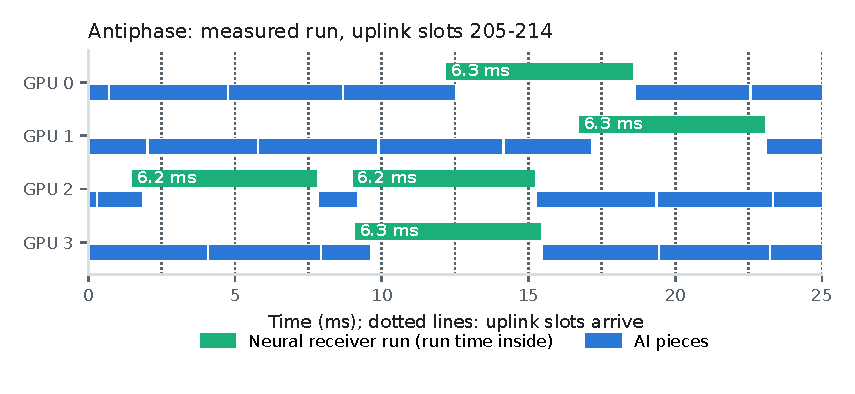
\includegraphics[width=0.9\linewidth]{figures/timeline_server.pdf}
\caption{Measured timeline of the four GPUs under \sys (16 cells, full load, 25~ms).}
\label{fig:timeline}
\end{figure}

Figure~\ref{fig:timeline} shows the rule on a measured run. A neural receiver starts on GPU~2 at 1.5~ms.
The AI piece of that GPU ends 0.3~ms later, and AI starts again when the neural receiver ends at 7.8~ms.
The neural receiver runs take 6.2-6.3~ms, as without AI. The AI workers of the GPUs without a running
neural receiver continue.

\noindent\textbf{AI Requests.} Requests arrive in one list for the server. The controller predicts when a
new request would finish on each GPU from the waiting work with the same or a shorter time limit and from
the recent service rate of the GPU. It places the request on the GPU that finishes it first and rejects it
if no GPU finishes it within 75\% of its limit. Inside a piece, the worker runs first the unit of the job
whose next result is due earliest after its remaining work. Embedding and image items wait for a batch for
up to 30\% of their limit. Every baseline uses the same placement, rejection, and order.

\noindent\textbf{Time Bounds.} The bounds come from measurements on the evaluation hardware with all cells
running. The larger neural receiver takes 6.3-6.4~ms at the median next to four or five cells, and its
bound is 7.6~ms. The bound sets the latest start time of a candidate: a larger bound has fewer runs that
end after the recovery deadline and an earlier latest start time, and Section~\ref{sec:cells} chooses it
with the model. A size class is allowed next to the conventional receivers if they finish before the
layer-1 deadline at the 99.9th percentile next to continuously running low-priority units of that class.
With four cells per GPU, the receivers of the single-user cells finish in 3.65, 3.86, and 4.05~ms next to
128-, 512-, and 1,024-token units, and \sys allows the two smaller classes.

\noindent\textbf{Implementation.} The neural receiver path is the public TensorRT export of the NVlabs
model followed by rate recovery, LDPC decoding, and CRC from cuPHY. We replace the least-squares channel
estimation call with one multiplication of the pilot samples and call the cuPHY bit-level functions on
buffers allocated once, which shortens the path of the real-time model from 3.08 to 2.36~ms with the same
decoded TBs. The run-time path of the real-time model agrees with the NVlabs evaluation on 794 of 800 TBs.
\sys is 4.1k lines of Python over cuPHY, TensorRT, and PyTorch.

\section{Evaluation}
\label{sec:eval}

\subsection{Evaluation setup}

\noindent\textbf{Hardware.} One node with four NVIDIA A100 80~GB GPUs under MPS and 64 CPU cores.

\noindent\textbf{Scope.} All measurements are end-to-end runs on the GPUs: cuPHY decodes every TB, the
neural receiver decodes real received slots, and the AI worker runs real models. The slots are generated in
advance; there is no radio unit and no layer-2 stack.

\noindent\textbf{Workloads.} Sixteen cells run on four GPUs, four per GPU, unless stated. One cell per GPU
carries two users on the same 273 PRBs (16QAM, 20 code blocks per slot); the other cells carry one user
with two layers. The two-user slots come from three channels of the NVlabs link simulation: low
correlation at 2-3~dB, high correlation at 13-16~dB, and urban micro~\cite{tr38901} at 4-6~dB. Every cell
replays 512 slots (1.28~s). Both receivers run 20 LDPC iterations, the neural receiver is the larger NVlabs
model, $K=9$, and the recovery deadline is 11.5~ms. AI requests are Qwen2.5-1.5B~\cite{qwen25} prefill
requests of up to 1,024 tokens with lengths from BurstGPT~\cite{burstgpt} and a 200~ms limit, offered at 32
requests/s per GPU (53k tokens/s for the server) unless stated. A request that finishes after the limit
does not count. Section~\ref{sec:kinds} adds output tokens, a larger LLM, text embedding~\cite{bge}, and
image classification~\cite{vit}. Runs last 10-40~s; values are means over five seeds unless stated.

\noindent\textbf{Metrics.} \emph{AI served} is the prompt tokens per second of requests that finish within
the limit. \emph{Recoveries kept} is the number of TBs that the neural receiver recovers before the recovery
deadline as a share of the run without AI on the same seed; run-to-run variation moves it by a few tenths of
a percent, and it can exceed 100\%. \emph{Recoveries lost} is 100\% minus the recoveries kept.
\emph{Layer-1 misses} is the share of TBs whose conventional result
passes the layer-1 deadline; in a run of 10-40~s most of them fall into the first seconds after the processes
start (Section~\ref{sec:protect}). \emph{Lost candidates} is the share of candidates that find no free neural
receiver by their latest start time.

\noindent\textbf{Baselines.} Every policy uses the same recovery path, the same AI requests, and the same
placement and rejection of AI requests. The policies differ in when AI may use the GPU.
\begin{itemize}
\item \textit{Static} gives the AI worker a fixed MPS share of 10\%, a static split of the GPU between
radio and AI. It is the largest share we measured that keeps the recoveries at full load; a 30\% share
loses 4.9\% of them.
\item \textit{Priority} adds a low MPS priority for the AI worker, the mechanism that SMEC applies on an
edge server~\cite{smec}, with a cap of 30\% on the share. \textit{Priority-70} and \textit{Priority-max}
use a cap of 70\% and no cap; they serve more AI and lose recoveries.
\item \textit{Estimator} follows the design of YinYangRAN~\cite{yinyangran}. Every second
it picks the largest AI share for which an estimator predicts that the reliability targets hold, given the
histogram of the radio load of the last second. The estimator is a neural network trained offline with a
quantile loss on runs at four steady loads and every share, with a seed that the evaluation does not use.
The targets are 97\% of the recoveries and 99.9\% of the TBs within the layer-1 deadline. A change of share
stops AI for 0.27~s, the MPS reconfiguration time that YinYangRAN reports. \textit{Estimator+Priority} runs
it with low-priority AI.
\item \textit{Follow+Priority} is an idealized form of the same idea with low-priority AI: it keeps one AI
worker per share loaded on every GPU and makes the worker of a lower share active when the radio load of
the last 100~ms is higher. It knows the load at once and has no switching cost. \textit{Follow} is the
same without low priority.
\end{itemize}
In the tables, \textit{Static} is the fixed 10\% share and \textit{Priority} is the 30\% share with
low-priority AI.
The baselines are the mechanisms of these systems on our code, not the systems. The estimator baseline is
favored in two ways: the radio work stays on the GPU during a reconfiguration, and no model is reloaded.

\subsection{Summary of results}
\label{sec:summary}

\begin{figure}[t]
\centering
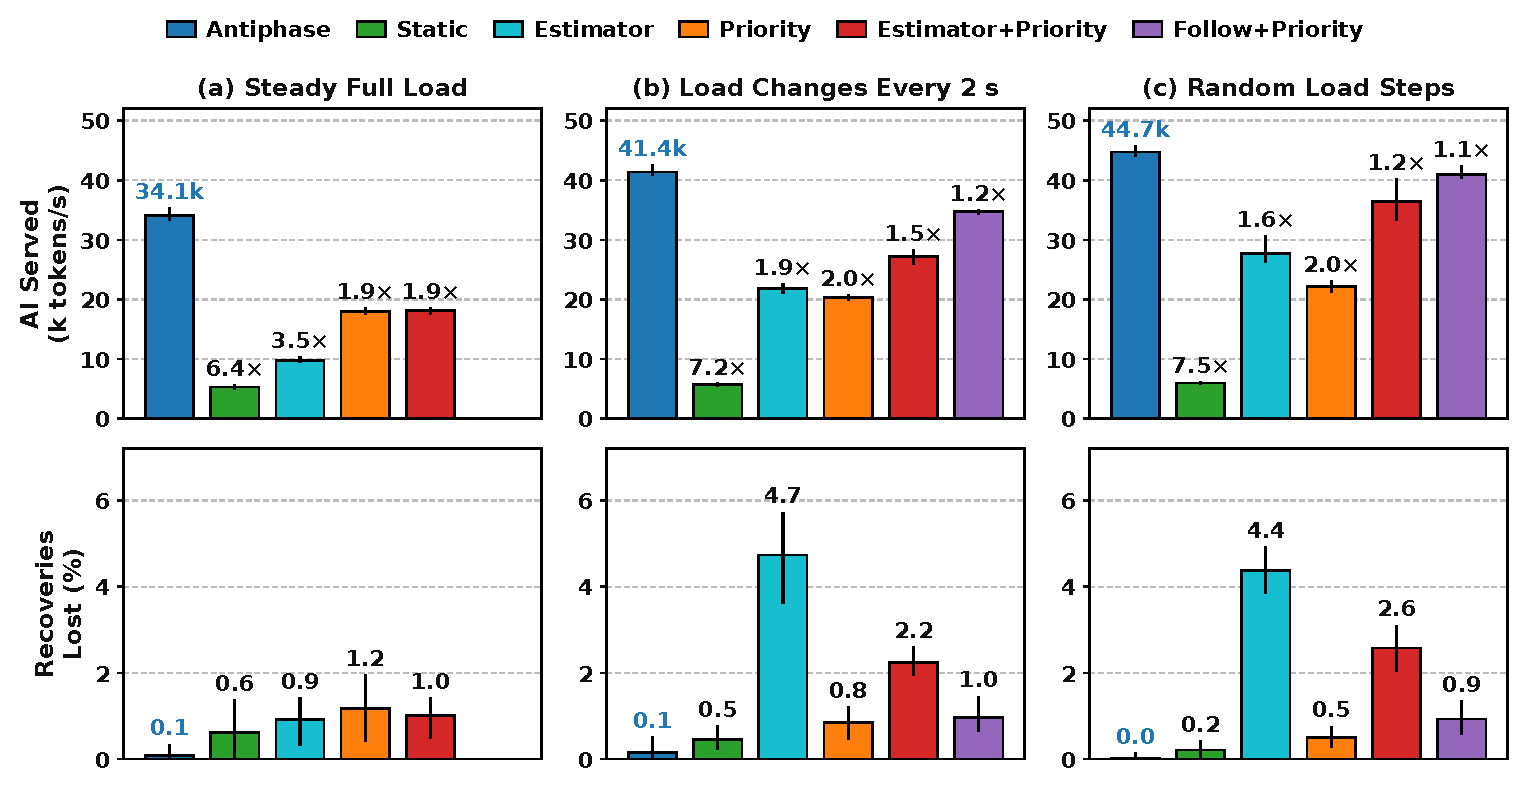
\includegraphics[width=\linewidth]{figures/eval_headline.pdf}
\caption{AI served (top) and recoveries lost (bottom) under three load patterns (16 cells, four GPUs, five
seeds; lines show the range over seeds). The number on a baseline is how many times more AI \sys serves
than that baseline.}
\label{fig:times}
\end{figure}

\begin{table}[t]
\caption{Main results with 16 cells on four GPUs. Factors are \sys over the compared baseline.}
\label{tab:summary}
\footnotesize
\setlength{\tabcolsep}{4pt}
\begin{tabular}{@{}llll@{}}
\toprule
Result & \sys & Compared with & Factor \\
\midrule
AI served, steady full load & 34.1k tokens/s & \textit{Static} (5.3k) & 6.4$\times$ \\
 & & \textit{Priority} (18.0k) & 1.9$\times$ \\
 & & \textit{Estimator+Priority} (18.1k) & 1.9$\times$ \\
AI served, load changes every 2~s & 41.4k tokens/s & \textit{Static} (5.7k) & 7.2$\times$ \\
 & & \textit{Estimator+Priority} (27.2k) & 1.5$\times$ \\
 & & \textit{Follow+Priority} (34.7k) & 1.2$\times$ \\
AI served, random load steps & 44.7k tokens/s & \textit{Static} (6.0k) & 7.5$\times$ \\
 & & \textit{Estimator+Priority} (36.4k) & 1.2$\times$ \\
Recoveries lost & 0.0-0.1\% & \textit{Priority-70} (2.7-5.6\%) & \\
Layer-1 latency added, 99.9th percentile & 0.04-0.06~ms & baselines (0.14-0.87~ms) & 2.8-21$\times$ less \\
GPU time safe for AI that is used & 70\% & \textit{Static} to \textit{Priority} (11-37\%) & 1.9-6.4$\times$ \\
Goodput lost by two-user cells, 42 settings & at most 0.4\% & \textit{Priority-max} (up to 8.2\%) & \\
Loss model & 0.82 points error & 672 measured runs & \\
\bottomrule
\end{tabular}
\end{table}

Figure~\ref{fig:times} and Table~\ref{tab:summary} summarize the evaluation. At a steady full load
(Figure~\ref{fig:times}a), \sys serves 34.1k tokens/s, which is 6.4$\times$ \textit{Static} (5.3k),
3.5$\times$ \textit{Estimator} (9.8k), and 1.9$\times$ \textit{Priority} and \textit{Estimator+Priority}
(18.0k and 18.1k). \sys loses 0.1\% of the recoveries, and the baselines lose 0.6-1.2\%. When the load
changes every 2~s (Figure~\ref{fig:times}b), \sys serves 41.4k tokens/s, 7.2$\times$ \textit{Static},
2.0$\times$ \textit{Priority}, and 1.5$\times$ \textit{Estimator+Priority}. The two estimator policies
lose 4.7\% and 2.2\% of the recoveries, because their decision is one second behind the load, and \sys
loses 0.1\%. \textit{Follow+Priority} knows the load without lag and serves 34.7k; \sys serves
1.2$\times$ more. With random load steps (Figure~\ref{fig:times}c), \sys serves 44.7k tokens/s,
7.5$\times$ \textit{Static} and 1.1-2.0$\times$ the other baselines, and keeps 100.0\% of the recoveries. In
all three patterns \sys loses the fewest recoveries and serves the most AI of the policies in
Figure~\ref{fig:times}. \textit{Priority-70} and
\textit{Priority-max} serve 1.1-1.4$\times$ the AI of \sys and lose 2.7-6.3\% of the recoveries
(Section~\ref{sec:steady}).

\subsection{Model validation}
\label{sec:modelval}

\noindent\textbf{Takeaway.} The closed form predicts the lost candidates of 672 runs with a mean absolute
error of 0.82 percentage points and has no fitted parameter.

\begin{figure}[t]
\centering
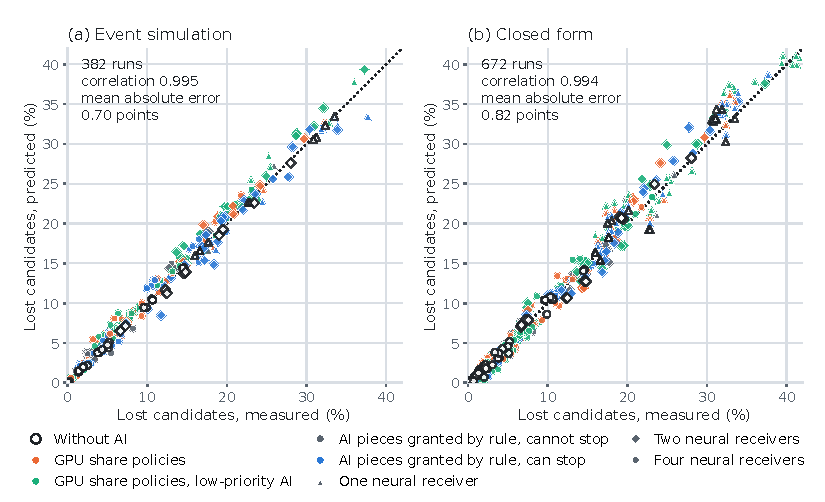
\includegraphics[width=\linewidth]{figures/loss_model.pdf}
\caption{Share of the candidates that find no free neural receiver, predicted against measured, for every
run. GPU share policies: fixed share, share that follows the load, and share chosen by an estimator.}
\label{fig:model}
\end{figure}

\begin{table}[t]
\caption{Model against measurement: share of the candidates that find no free neural receiver. Errors are
in percentage points. The first 412 runs existed when the model was built.}
\label{tab:model}
\footnotesize
\begin{tabularx}{\linewidth}{@{}>{\raggedright\arraybackslash}p{0.27\linewidth}>{\raggedright\arraybackslash}Xrrrr@{}}
\toprule
Form & Inputs besides $N$ & Runs & Correlation & Mean absolute & Mean \\
 & & & & error & error \\
\midrule
Event simulation & arrivals without AI, $S$ alone and next to AI, rule & 334 & 0.995 & 0.77 & $+$0.46 \\
Closed form & $T$, distributions of $c$ and $S$ & 672 & 0.994 & 0.82 & $+$0.06 \\
Closed form, first runs & same & 412 & 0.993 & 0.95 & $+$0.07 \\
Closed form, runs measured after the model was final & same & 260 & 0.996 & 0.61 & $+$0.06 \\
Closed form with measured $f$ & $T$, $f$ & 412 & 0.993 & 0.92 & $-$0.14 \\
Closed form with measured $f$ and independent arrivals & mean arrival rate, $f$ & 412 & 0.972 & 2.87 & $-$2.76 \\
\bottomrule
\end{tabularx}
\end{table}

We compare the closed form with 672 runs: one, two, and four neural receivers (106, 78, and 488 runs), 4-48
cells with one to twelve two-user cells, and 35 policies and settings. Figure~\ref{fig:model} and
Table~\ref{tab:model} show the result. The closed form takes the distributions of $c$ and $S$ from the runs
of the same policy with other seeds. Its mean absolute error is 0.48 points with four neural receivers, 1.45
with two, and 1.93 with one, over a range of 0-42\% lost candidates. The share of three-slot runs that it
computes agrees with the measured share within 3.4 points on average. Giving the closed form the measured
share does not make it more accurate. Assuming independent arrivals makes it underestimate the loss by more
than half.

\noindent\textbf{Runs Measured After the Model Was Final.} The model has no fitted parameter. To test it on
settings that we had not seen when we built it, we measured 260 more runs: other AI loads, AI requests in
bursts, 20, 32, and 48 cells, a second latest start time, three more seeds with one GPU, and changing and
bursty radio loads (Section~\ref{sec:cells}). The mean absolute error on these runs is 0.61 points. It is
0.06-0.62 points per setting, except with one GPU, where the closed form is 2.5 points high, and with 2~s
bursts on 32 cells, where it is 1.4 points low: the closed form describes the arrivals by one transition
matrix and does not see the load change over seconds.

\begin{table}[t]
\caption{Lost candidates per setting: measured / closed form (\%). In parentheses: share of three-slot
runs, measured $\rightarrow$ closed form (\%).}
\label{tab:modelcond}
\footnotesize
\begin{tabular}{@{}llll@{}}
\toprule
Neural receivers, two-user cells & No AI & \sys & 70\%, low-priority AI \\
\midrule
4, 2 & 0.0 / 0.1 (4 $\rightarrow$ 3) & 0.0 / 0.1 (7 $\rightarrow$ 5) & 1.3 / 1.0 (78 $\rightarrow$ 77) \\
4, 4 & 1.6 / 1.6 (10 $\rightarrow$ 7) & 1.7 / 1.9 (11 $\rightarrow$ 10) & 6.2 / 5.7 (86 $\rightarrow$ 86) \\
4, 6 & 4.7 / 4.4 (14 $\rightarrow$ 13) & 4.8 / 4.7 (17 $\rightarrow$ 16) & 11.4 / 12.0 (90 $\rightarrow$ 91) \\
4, 8 & 10.1 / 10.5 (21 $\rightarrow$ 22) & 10.5 / 10.9 (23 $\rightarrow$ 24) & 19.7 / 20.4 (89 $\rightarrow$ 91) \\
2, 2 & 7.0 / 7.5 (14 $\rightarrow$ 10) & 7.2 / 8.0 (16 $\rightarrow$ 15) & 14.1 / 14.2 (78 $\rightarrow$ 78) \\
2, 4 & 19.3 / 20.7 (21 $\rightarrow$ 20) & 19.4 / 21.1 (24 $\rightarrow$ 24) & 28.8 / 30.0 (83 $\rightarrow$ 85) \\
1, 1 & 16.8 / 17.3 (5 $\rightarrow$ 6) & 17.0 / 18.0 (13 $\rightarrow$ 13) & 24.1 / 22.7 (65 $\rightarrow$ 63) \\
1, 2 & 30.9 / 33.0 (8 $\rightarrow$ 14) & 31.9 / 33.8 (19 $\rightarrow$ 20) & 40.3 / 40.0 (69 $\rightarrow$ 72) \\
\bottomrule
\end{tabular}
\end{table}

Table~\ref{tab:modelcond} gives the values per setting. In all eight settings, \sys loses at most 1.0 point
more candidates than the run without AI, and \textit{Priority-70} loses 1.3-9.6 points more.
The model is least accurate for \textit{Priority} on one and two neural receivers, where
the closed form is 2.4-3.8 points high: a fixed share slows the neural receiver only while AI is active, and
the closed form draws the run length of every run independently.

\begin{figure}[t]
\centering
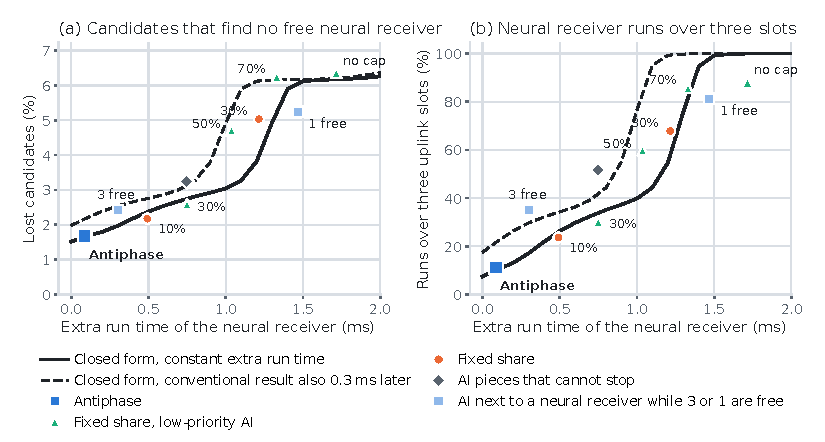
\includegraphics[width=\linewidth]{figures/loss_sensitivity.pdf}
\caption{Lost candidates and three-slot runs against the extra run time of the neural receiver (16 cells,
four neural receivers). Lines: closed form with the arrivals and run lengths of the run without AI plus a
constant extra run time. Points: measured policies at their median extra run time; labels give the MPS
shares.}
\label{fig:sensitivity}
\end{figure}

\noindent\textbf{Extra Run Time.} Figure~\ref{fig:sensitivity} tests the slack of
Equation~\ref{eq:slack}. The closed form gives 1.5\% lost candidates with no extra run time, 3.0\% with
1.0~ms, and 5.9\% with 1.4~ms, where 95\% of the runs take three slots. When the conventional result is
also 0.3~ms late, as it is next to AI, the step moves 0.3~ms to the left. The 13 measured policies lie
between the two lines or within 0.3 points of them; one setting that allows AI next to a neural receiver
while one other is free is 0.8 points below. \sys adds 0.09~ms to the run of the neural receiver and loses
1.7\% of the candidates, against 1.6\% without AI. The 30\% shares add 0.75-1.21~ms and lose 2.6-5.0\%, and
\textit{Priority-70} adds 1.33~ms and loses 6.2\%.

\noindent\textbf{A Bias of Slot Replay.} The model exposed a bias of our own method. Earlier runs replayed
128 slots per cell (0.32~s). The slots in which the failures of several cells coincide then repeat every
0.32~s, and the loss without AI was 1.45\% and 3.76\% for two seeds, which the closed form did not
reproduce. With 512 slots the two seeds give 1.30\% and 1.34\%, and the recoveries kept by the baselines
rise by 1.0-1.5 points. Every result in this section uses 512 slots.

\subsection{AI served at a steady full load}
\label{sec:steady}

\noindent\textbf{Takeaway.} At a steady full load \sys serves 6.4$\times$ the AI of \textit{Static} and
1.9$\times$ that of the best existing mechanism that keeps the recoveries, and it keeps 99.9\% of the
recoveries.

\begin{figure}[t]
\centering
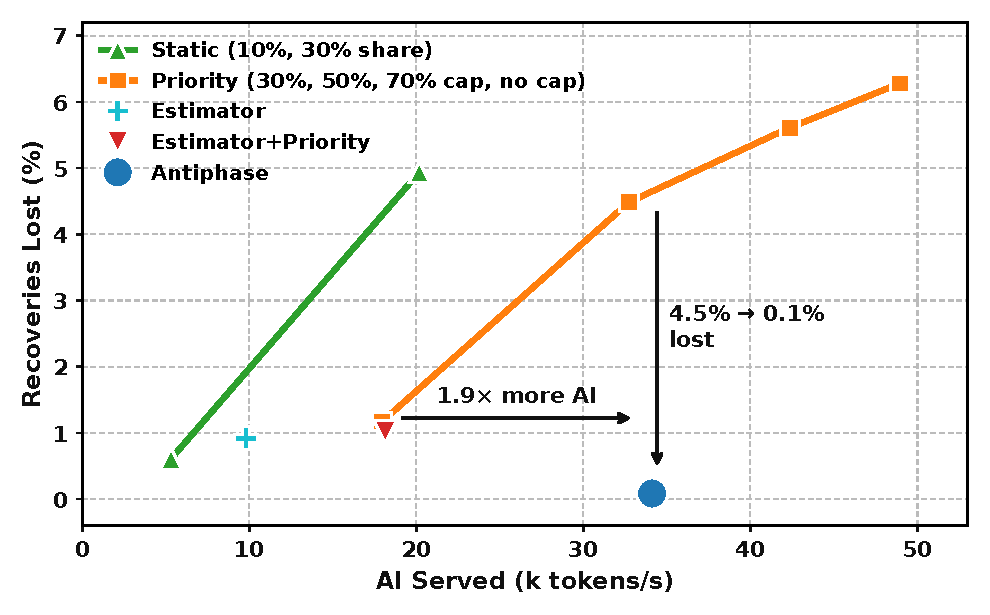
\includegraphics[width=0.72\linewidth]{figures/eval_tradeoff.pdf}
\caption{AI served against recoveries lost at a steady full load (16 cells, four GPUs). A baseline that
takes a larger share moves up along its line.}
\label{fig:tradeoff}
\end{figure}

\begin{table}[t]
\caption{Steady full load, 16 cells, 53k tokens/s offered (range over seeds in parentheses; five seeds,
rows marked $^{*}$ two).}
\label{tab:steady}
\footnotesize
\begin{tabular}{@{}llll@{}}
\toprule
Policy & AI tokens/s within 200~ms & Recoveries kept & Layer-1 misses \\
\midrule
\sys & 34.1k (33.4-35.3k) & 99.9\% (99.7-100.3\%) & 0.036\% \\
Fixed 10\% & 5.3k (5.1-5.6k) & 99.4\% (98.7-99.9\%) & 0.032\% \\
Fixed 30\%$^{*}$ & 20.2k (20.1-20.3k) & 95.1\% (94.9-95.2\%) & 0.051\% \\
Fixed 30\%, low-priority AI & 18.0k (17.6-18.5k) & 98.8\% (98.1-99.6\%) & 0.037\% \\
Fixed 50\%, low-priority AI$^{*}$ & 32.7k (32.5-33.0k) & 95.5\% (95.5-95.5\%) & 0.040\% \\
Fixed 70\%, low-priority AI & 42.4k (41.1-43.4k) & 94.4\% (93.6-95.1\%) & 0.037\% \\
Low-priority AI, no cap & 49.0k (47.5-49.9k) & 93.7\% (93.4-94.5\%) & 0.044\% \\
Share chosen by an estimator & 9.8k (9.5-10.3k) & 99.1\% (98.6-99.7\%) & 0.019\% \\
Share chosen by an estimator, low-priority AI & 18.1k (17.7-18.4k) & 99.0\% (98.6-99.5\%) & 0.018\% \\
No AI & 0 & 100\% & 0.032\% \\
\bottomrule
\end{tabular}
\end{table}

Figure~\ref{fig:tradeoff} and Table~\ref{tab:steady} show AI served against recoveries with all 16
cells at full load. The run without AI recovers 187 TBs per second. A baseline cannot reach \sys by taking
more GPU time. Raising the cap of \textit{Priority} from 30\% to 50\% brings its AI to 32.7k tokens/s,
close to \sys, and its lost recoveries from 1.2\% to 4.5\%; \sys serves 34.1k and loses 0.1\%. A 30\%
share for \textit{Static} serves 20.2k and loses 4.9\%.

\noindent\textbf{Recoveries and Layer 1.} \sys keeps 99.9\% of the recoveries. It misses the layer-1
deadline for 0.036\% of the TBs against 0.032\% without AI, and the conventional receivers finish in 3.14~ms
at the 99.9th percentile against 3.10~ms without AI and 3.51~ms under \textit{Priority-70}.

\noindent\textbf{AI Served.} \sys serves 34.1k tokens/s. Among the existing mechanisms that keep at least
98.8\% of the recoveries, \textit{Estimator+Priority} and \textit{Priority} serve
the most, 18.1k and 18.0k; \sys serves 1.9$\times$ more. It serves 6.4$\times$ more than the fixed 10\%
share and 3.5$\times$ more than the estimator without low priority. At a steady full load the estimator
settles on a share of 20\%, or 30\% with low-priority AI, and equals that fixed share. The 70\% share with
low-priority AI and \textit{Priority-max} serve 24\% and 44\% more AI than \sys and lose 5.6\% and 6.3\% of the
recoveries.

\subsection{AI served under a changing load}

\noindent\textbf{Takeaway.} When the radio load changes, \sys serves 7.2-7.5$\times$ the AI of a fixed 10\%
share and 1.2-1.5$\times$ that of \textit{Estimator+Priority}, and it keeps 2.1-2.6 points more
recoveries than that policy.

\begin{table}[t]
\caption{Changing load, 16 cells, five seeds. Each cell shows AI tokens/s within 200~ms and recoveries
kept.}
\label{tab:changing}
\footnotesize
\begin{tabular}{@{}lll@{}}
\toprule
Policy & Full and half load, every 2~s & Random steps, 25-100\% \\
\midrule
\sys & 41.4k, 99.9\% & 44.7k, 100.0\% \\
Fixed 10\% & 5.7k, 99.5\% & 6.0k, 99.8\% \\
Fixed 30\%, low-priority AI & 20.3k, 99.2\% & 22.2k, 99.5\% \\
Fixed 70\%, low-priority AI & 46.9k, 96.0\% & 48.6k, 97.3\% \\
Share follows the load & 23.8k, 99.2\% & 30.0k, 98.6\% \\
Share follows the load, low-priority AI & 34.7k, 99.0\% & 40.9k, 99.1\% \\
Share chosen by an estimator & 21.8k, 95.3\% & 27.7k, 95.6\% \\
Share chosen by an estimator, low-priority AI & 27.2k, 97.8\% & 36.4k, 97.4\% \\
\bottomrule
\end{tabular}
\end{table}

\noindent\textbf{Alternating Load.} The radio load alternates every two seconds between full load and each
cell active with probability 0.5. Figure~\ref{fig:times} and Table~\ref{tab:changing} show the result.
\sys serves 41.4k tokens/s and keeps 99.9\% of the recoveries, with layer-1 misses of 0.019\% against 0.018\%
without AI. This is 7.2$\times$ the AI of \textit{Static}. The estimator serves 21.8k tokens/s and keeps
95.3\%: its decision rests on the load of the last second, and its shares run one second behind the load,
at 70\% for half of every full-load period. With low-priority AI it serves 27.2k at 97.8\%; \sys serves
1.5$\times$ more and keeps 2.1 points more recoveries. The share that follows the load at once and without a
switching cost serves 23.8k at 99.2\%, and 34.7k at 99.0\% with low-priority AI; \sys serves 1.2$\times$ more.
\textit{Priority-70} serves 13\% more AI than \sys and loses 4.0\% of the recoveries.

\noindent\textbf{Alternation Interval.} With a change every 0.2~s and every 5~s (two seeds), \sys serves
42.5k and 41.2k tokens/s and keeps 99.8\% of the recoveries in both. The policies that change the share
with the load lose more recoveries as the interval gets shorter. The estimator decides every second: it
keeps 94.0\% with a change every 0.2~s, where it misses the layer-1 deadline for 0.24\% of the TBs, and
97.9\% with a change every 5~s; with low-priority AI it keeps 96.6\% and 98.7\%. The share that follows the
load judges the load over 100~ms and keeps 97.3\% with a change every 0.2~s, 97.6\% with low-priority AI.

\noindent\textbf{Random Load Steps.} The share of active cells jumps between 25, 50, 75, and 100\% at random
times 0.5-1.5~s apart for 40~s. \sys serves 44.7k tokens/s and keeps 100.0\% of the recoveries. The
estimator with low-priority AI serves 36.4k at 97.4\%, and the share that follows the load with low-priority
AI serves 40.9k at 99.1\%. The difference comes from the periods of full load. There \sys serves 34.9k
tokens/s and keeps 100.0\%. The share that follows the load drops to its lowest share and serves 3.9k, or
20.4k with low-priority AI. \textit{Priority-70} and \textit{Estimator+Priority} serve
44.0k and 35.4k and keep 94.3\% and 94.7\%.

\noindent\textbf{Bursts.} When every cell switches on and off by itself with a mean busy run of 20~ms or
2~s (half load on average, two seeds), the neural receivers are needed half as often as at full load. With
16 cells, \sys serves 49.6k and 48.0k tokens/s and keeps 100.1\% and 99.8\% of the recoveries, and the 70\%
share with low-priority AI serves 51.1k and 50.4k and keeps 99.5\% and 98.6\%: at this load low priority
alone loses few recoveries. With 32 cells, \sys serves 33.5k and 34.4k tokens/s at 99.7\% and 99.1\%,
1.9$\times$ \textit{Priority}, and \textit{Priority-70} serves 22-23\% more
and loses 3.8-4.6\% of the recoveries. With 2~s runs, several cells of a GPU are busy for seconds, and the
layer-1 misses are 0.25\% with 16 cells and 1.1\% with 32 cells without AI. Every policy with AI misses more
(0.26-0.31\% and 1.3-1.9\%), and we do not compare the policies on the layer-1 deadline in this setting.

\subsection{What a recovery is worth}
\label{sec:worth}

\noindent\textbf{Takeaway.} The recovery path raises the goodput of two-user cells by 5.6\% at a fixed MCS
and by 11-40\% under closed-loop rate control on a high-correlation channel. \sys loses at most 0.4\% of the
goodput in 42 settings, where the other policies
lose up to 8.2\%.

\begin{table}[t]
\caption{Uplink goodput with the retransmission schedule applied to the TB records of the runs of
Table~\ref{tab:steady} (two-user cells).}
\label{tab:goodput}
\footnotesize
\begin{tabular}{@{}lrrr@{}}
\toprule
Policy & Goodput against & Retransmissions & Delay (ms), mean / \\
 & no recovery path & per 100 TBs & 99th percentile \\
\midrule
No recovery path & 0 & 16.9 & 5.77 / 12.0 \\
Recovery path, no AI & $+$5.61\% & 10.7 & 5.64 / 17.0 \\
\sys & $+$5.63\% & 10.7 & 5.66 / 17.0 \\
Fixed 10\% & $+$5.60\% & 10.7 & 5.67 / 17.0 \\
Share chosen by an estimator, low-priority AI & $+$5.58\% & 10.7 & 5.69 / 17.0 \\
Fixed 30\%, low-priority AI & $+$5.57\% & 10.7 & 5.69 / 17.0 \\
Fixed 70\%, low-priority AI & $+$5.31\% & 11.0 & 5.72 / 17.0 \\
Low-priority AI, no cap & $+$5.27\% & 11.1 & 5.75 / 17.0 \\
\bottomrule
\end{tabular}
\end{table}

\noindent\textbf{Goodput.} We apply the retransmission schedule to the per-TB records of the runs. A TB that
the neural receiver recovers needs no retransmission; a TB that is not a candidate or gets no neural
receiver is retransmitted 7.5~ms after its slot, as without a recovery path; a TB whose neural receiver run
fails is retransmitted 5~ms later. A retransmission succeeds with probability 0.95 and takes one uplink
slot from new data. Table~\ref{tab:goodput} shows that the recovery path raises the goodput of two-user
cells by 5.6\% and cuts the retransmissions per 100 TBs from 16.9 to 10.7. The policies differ little: one
percent of lost recoveries is 0.06 points of goodput, and \sys and \textit{Priority-max} are 0.36 points
apart. Over eight settings (full, alternating, and random load, eight two-user cells, two GPUs, and 20,
32, and 48 cells), the recovery path adds 4.6-5.9\% of goodput, \sys keeps that gain within 0.03 points,
and one percent of lost recoveries costs 0.05-0.06 points. The largest gap is with eight two-user cells,
where \sys and \textit{Priority-70} are 0.59 points apart ($+$5.26\% against $+$4.67\%). Thus, the result of \sys in goodput is that it keeps the gain of the recovery path while serving
34.1k tokens/s, where the existing mechanisms that keep the same gain serve 5.3k-18.1k. The 99th-percentile
delay grows from 12 to 17~ms with the recovery path, because the retransmission of a failed recovery is
5~ms late; the mean delay falls. A user of a two-user cell has 2.5 HARQ processes in use on average and at
most six with and without the recovery path, within the 16 that NR allows~\cite{ts38214}.

\begin{figure}[t]
\centering
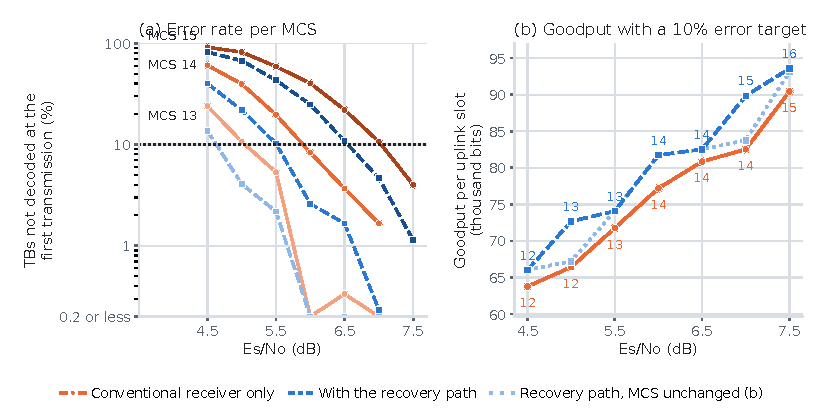
\includegraphics[width=\linewidth]{figures/link_adaptation.pdf}
\caption{Link adaptation with the recovery path (two-user cell, low-correlation channel, 300 TBs per
point). Dotted line in (a): 10\% target. Numbers in (b): MCS chosen.}
\label{fig:la}
\end{figure}

\begin{table}[t]
\caption{Link adaptation with the recovery path on the three channels of the workload (two-user cell, MCS
10-16, 200-600 TBs per point). Gains are in goodput with a 10\% target for first-transmission errors.}
\label{tab:la}
\footnotesize
\begin{tabular}{@{}llrrrl@{}}
\toprule
Channel & Es/No (dB) & Shift of the & Gain, MCS & Gain, MCS chosen & Points with \\
 & & 10\% point (dB) & unchanged & with the recovery path & a higher MCS \\
\midrule
Low correlation & 4.5-7.5 & 0.4-0.5 & $+$2.9\% & $+$5.2\% & 3 of 7 \\
High correlation & 12-24 & 2.5-4.0 & $+$5.2\% & $+$11.8\% & 6 of 7 \\
Urban micro & 4-14 & 0.2-1.5 & $+$1.6\% & within the statistical error & none confirmed \\
\bottomrule
\end{tabular}
\end{table}

\noindent\textbf{Link Adaptation.} A recovery path may allow a higher modulation and coding scheme (MCS).
We decode the same slots with both receivers for MCS 10-16 at fixed Es/No points on the three channels of
the workload (Table~\ref{tab:la}; Figure~\ref{fig:la} shows the low-correlation channel). The larger model
outputs 16QAM soft bits, and one engine serves every code rate. On the low-correlation channel, the recovery
path moves the point of 10\% first-transmission errors by 0.4-0.5~dB, where one MCS step is 0.8-1.1~dB. A
rate controller with a 10\% target picks one MCS step higher at three of seven points, and the goodput
rises by 5.2\%, against 2.9\% with the MCS unchanged. On the high-correlation channel, the error rate of
the conventional receiver falls slowly with the SNR, and the recovery path moves the 10\% point by
2.5-4.0~dB. The rate controller picks one MCS step higher at six of seven points, and the goodput rises by
11.8\%, against 5.2\% with the MCS unchanged; at four of these points the conventional receiver fails
16-19\% of the TBs at the higher MCS. On the urban micro channel, the neural receiver decodes few of the
failed TBs: the goodput rises by 1.6-2.1\%, and no MCS step is outside the statistical error. With the
target itself as a parameter, the conventional receiver alone is best at a 10\% target on the
low-correlation channel, and with the recovery path the best target is 20-30\%, 5.5\% above; on the
high-correlation channel the best targets are 7.5\% apart. A higher MCS raises the neural receiver demand,
which takes GPU time from AI (Table~\ref{tab:scale}).

\begin{table}[t]
\caption{Closed-loop link adaptation: two-user cells on the high-correlation channel at 16~dB choose the MCS
of every slot by an outer loop. Target: share of TBs that need a retransmission. Policy cells: AI served
(tokens/s) / goodput of the two-user cells against the same server without AI. Rows without a cell count
have one two-user cell per GPU.}
\label{tab:closedloop}
\footnotesize
\setlength{\tabcolsep}{2.5pt}
\begin{tabular}{@{}lrrrrrrr@{}}
\toprule
 & \multicolumn{2}{c}{Recovery path, no AI} & & & \multicolumn{3}{c}{Low-priority AI} \\
\cmidrule(lr){2-3}\cmidrule(l){6-8}
Server, target & Goodput & Mean MCS, & \sys & Fixed 10\% & 30\% share & 70\% share & No cap \\
 & gain & without / with & & & & & \\
\midrule
4 GPUs, 10\% & $+$12.0\% & 12.5 / 13.5 & 11.4k / 0.0\% & 4.6k / $-$0.1\% & 11.5k / $-$0.3\% & 25.4k / $-$0.7\% & 30.1k / $-$1.0\% \\
4 GPUs, 3\% & $+$31.1\% & 10.7 / 12.8 & 19.8k / $+$0.2\% & 5.0k / $+$0.2\% & 14.0k / $-$0.1\% & 32.8k / $-$0.7\% & 39.4k / $-$1.4\% \\
4 GPUs, 1\% & $+$31.0\% & 10.0 / 12.1 & 33.7k / $-$0.1\% & 5.6k / $-$0.2\% & 18.0k / $-$0.4\% & 41.9k / $-$0.8\% & 49.0k / $-$2.3\% \\
8 two-user cells, 3\% & $+$25.9\% & 10.7 / 12.4 & 6.8k / $-$0.2\% & 4.4k / $-$0.7\% & 10.3k / $-$1.2\% & 21.5k / $-$2.0\% & 28.2k / $-$3.9\% \\
8 two-user cells, 1\% & $+$26.5\% & 10.0 / 11.8 & 17.0k / $-$0.3\% & 5.0k / $-$1.1\% & 14.3k / $-$2.3\% & 34.1k / $-$3.7\% & 45.5k / $-$8.2\% \\
2 GPUs, 10\% & $+$10.9\% & 12.5 / 13.4 & 7.0k / $-$0.1\% & 2.2k / $-$0.3\% & 5.9k / $-$0.3\% & 14.7k / $-$0.8\% & 17.0k / $-$1.0\% \\
2 GPUs, 3\% & $+$26.0\% & 10.8 / 12.6 & 11.9k / $+$0.1\% & 2.4k / $-$0.2\% & 7.3k / $-$0.4\% & 18.2k / $-$1.1\% & 21.1k / $-$1.6\% \\
2 GPUs, 1\% & $+$29.2\% & 10.0 / 11.9 & 17.6k / 0.0\% & 2.6k / $-$0.1\% & 9.0k / $-$0.9\% & 21.9k / $-$3.6\% & 24.7k / $-$4.6\% \\
1 GPU, 1\% & $+$24.4\% & 10.0 / 11.7 & 9.0k / 0.0\% & 1.1k / 0.0\% & 4.5k / $-$0.3\% & 10.2k / $-$2.4\% & 11.5k / $-$2.5\% \\
\bottomrule
\end{tabular}
\end{table}

\begin{figure}[t]
\centering
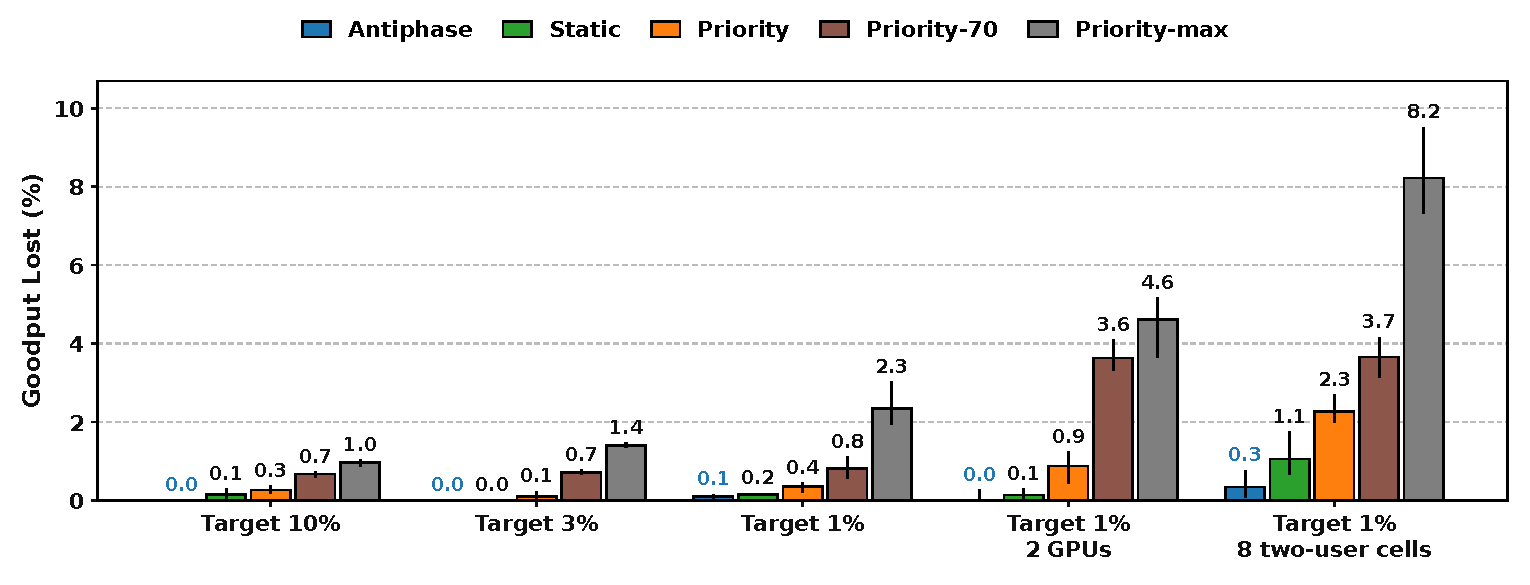
\includegraphics[width=\linewidth]{figures/eval_closed_loop.pdf}
\caption{Goodput of the two-user cells that each policy loses against the same server without AI, with an
outer-loop rate controller (target: share of TBs that need a retransmission; lines show the range over
seeds).}
\label{fig:closed}
\end{figure}

\noindent\textbf{Closed-Loop Rate Control.} The results above fix the MCS. We add an outer
loop~\cite{eolla} to the two-user cells. A cell holds the slots of MCS 10-16 on the high-correlation channel
at 16~dB and picks the MCS of every slot from a pointer over the levels. The pointer falls by 0.25 levels
for every TB that needs a retransmission and rises by $0.25\,\tau/(1-\tau)$ for every other TB, where
$\tau$ is the target share of TBs that need a retransmission; a TB that the neural receiver recovers before
the recovery deadline needs none. The outcome of a slot reaches the loop 15~ms later.
Figure~\ref{fig:closed} and Table~\ref{tab:closedloop} report the goodput of the two-user cells, the new
data per uplink slot of a user, over 18~s per run.

\noindent\textbf{The Recovery Path Is Worth More in Closed Loop.} With a 10\% target on four GPUs, the loop
without a recovery path settles at a mean MCS of 12.5 and the loop with it at 13.5: the goodput rises by
12.0\%. With 3\% and 1\% targets the gain is 24-31\%. On this channel the error rate of the conventional
receiver falls slowly with the MCS (1.4\% at MCS 10), and the loop without a recovery path gives up two MCS
levels to meet the target.

\noindent\textbf{Lost Recoveries Become a Lower MCS.} The share of TBs that need a retransmission equals the
target under every policy. A policy that loses recoveries spends more slots at the lower of two neighbouring
levels: the mean MCS falls by at most 0.64 levels, not by one level. One percent of lost candidates costs
0.09\% of goodput at the 10\% target, 0.15-0.37\% at 3\%, and 0.5-0.8\% at 1\%, against 0.06 points at a
fixed MCS. The error rate after recovery changes by 10.3 points per MCS level near the 10\% target and by
2.0 points near 1\%: the same rise of the error rate moves the loop five times as far.

\noindent\textbf{Where the Loss Is Visible.} With a 10\% target, the policies are within 1.0\% of each other
in goodput on two and four GPUs. With a 1\% target and a neural receiver demand near the capacity, the loss
grows: with eight two-user cells, \textit{Priority} and \textit{Priority-70} lose 2.3\% and
3.7\%, and \textit{Priority-max} loses 8.2\%; with two GPUs they lose 0.9\%, 3.6\%, and 4.6\%. \sys
stays within 0.4\% of the server without AI in all nine settings. In these two settings the 30\% share
with low-priority AI serves less AI than \sys (14.3k against 17.0k, 9.0k against 17.6k) and loses more goodput.

\noindent\textbf{What a Share Pays.} With a 10\% target, the loop raises the MCS until the neural receivers
run for 68\% of the time: 28.7\% of the slots of a two-user cell have a candidate, and 6.7\% of the
candidates find no neural receiver without any AI. \sys serves AI in the remaining time, 11.4k tokens/s,
and keeps the goodput. A share runs AI next to the running neural receivers. The 30\% share with
low-priority AI serves 11.5k and pays 0.3\% of the goodput, the 70\% share serves 25.4k and pays 0.7\%, and
low priority alone serves 30.1k and pays 1.0\%. The same three shares pay 2.3\%, 3.7\%, and 8.2\% with
eight two-user cells at the 1\% target: the price of a share is known only after the load is. The AI that
\sys serves follows the time in which the neural receivers are idle: 64\% at the 1\% target (33.7k,
1.9$\times$ the 30\% share), 46\% at the 3\% target (19.8k, 1.4$\times$), and 32\% at the 10\% target,
where it equals the AI of a 30\% share that runs all the time. With eight
two-user cells and a 3\% target, \sys serves 6.8k and stays within 0.2\%, and the 30\% share serves 10.3k
and pays 1.2\%. A server without the recovery path serves all 53.0k offered tokens/s with low-priority AI
and has 10.6\% less goodput in the two-user cells. With a step of 0.5 levels in the outer loop, the losses of the 70\%
share and of \textit{Priority-max} are 0.4\% and 0.6\% at the 10\% target, and those of the three low-priority
policies are 1.8\%, 3.1\%, and 6.5\% with eight two-user cells at the 1\% target; the order of the policies
is the same.

\begin{figure}[t]
\centering
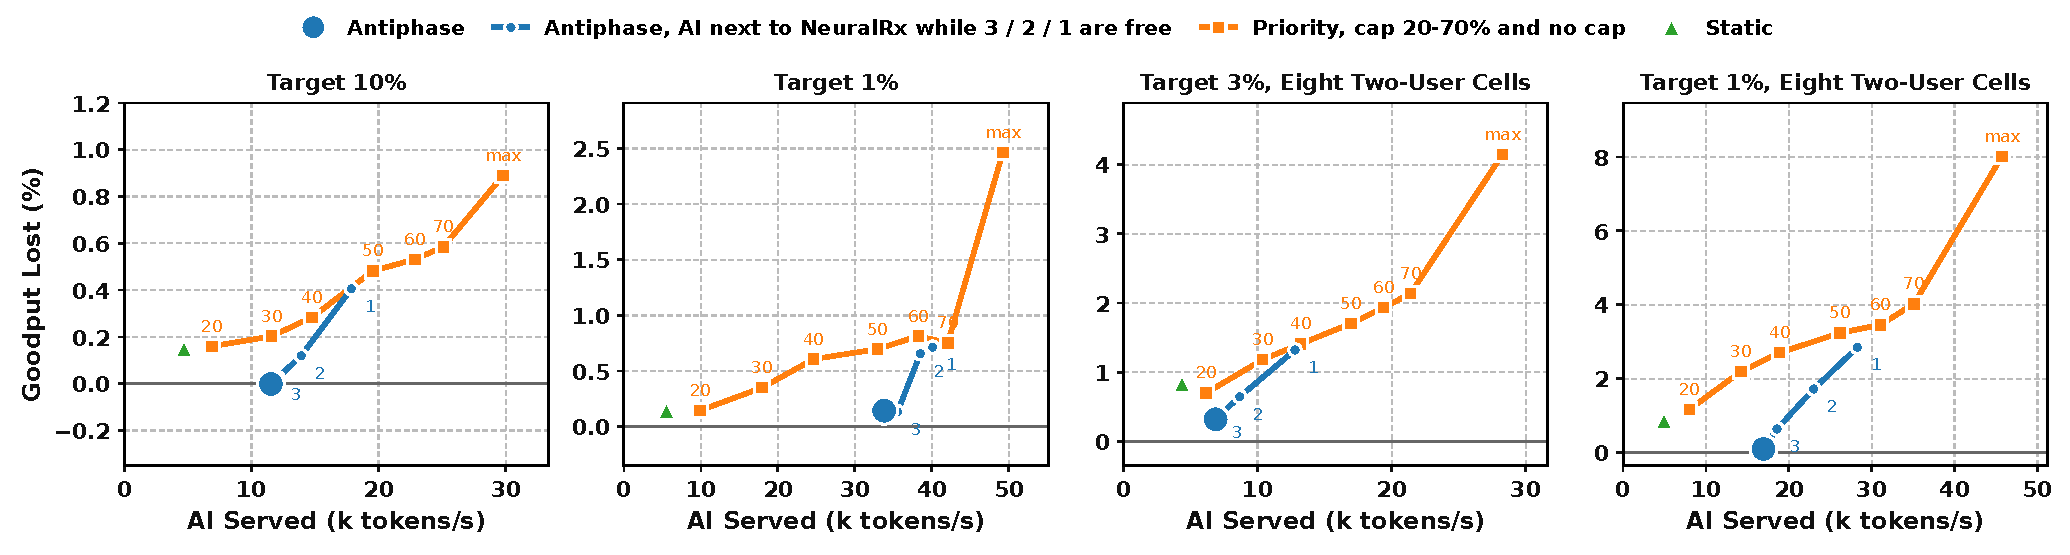
\includegraphics[width=\linewidth]{figures/eval_frontier.pdf}
\caption{AI served against the goodput of the two-user cells that is lost, with the outer loop (three seeds; all
policies of a panel run in one job). Orange: low-priority AI with a cap of 20-70\% and without a cap. Blue:
\sys, and its settings that allow AI next to a neural receiver while 3, 2, or 1 neural receivers are free.}
\label{fig:frontier}
\end{figure}

\noindent\textbf{No Cap Replaces the Rule.} A share with a well-chosen cap might keep the radio. We sweep the
cap of the low-priority share from 20\% to no cap in four settings (Figure~\ref{fig:frontier}). A higher cap
serves more AI and loses more goodput in every setting: from the 20\% cap to no cap, the loss grows from
0.2\% to 0.9\% at the 10\% target, from 0.2\% to 2.5\% at the 1\% target, and from 1.2\% to 8.0\% with
eight two-user cells at the 1\% target. The cap that keeps the goodput within 0.3\% depends on the setting:
it is 30\% at the 10\% target and 20\% at the 1\% target with four two-user cells, and with eight two-user
cells the fixed 10\% share already loses 0.8-0.9\%. \sys loses 0.0-0.3\% in the four settings with one
configuration. In no setting does a cap serve at least the AI of a setting of \sys at no more loss. Reading
the AI at a loss of at most 0.25\% from the lines between the measured points, \sys serves 1.2$\times$,
2.4$\times$, 2.2$\times$, and 7.8$\times$ the AI of the caps. The settings of \sys that allow AI next to a
neural receiver trade goodput for AI in the same way as a cap and from a lower loss; the default allows none.

\begin{figure}[t]
\centering
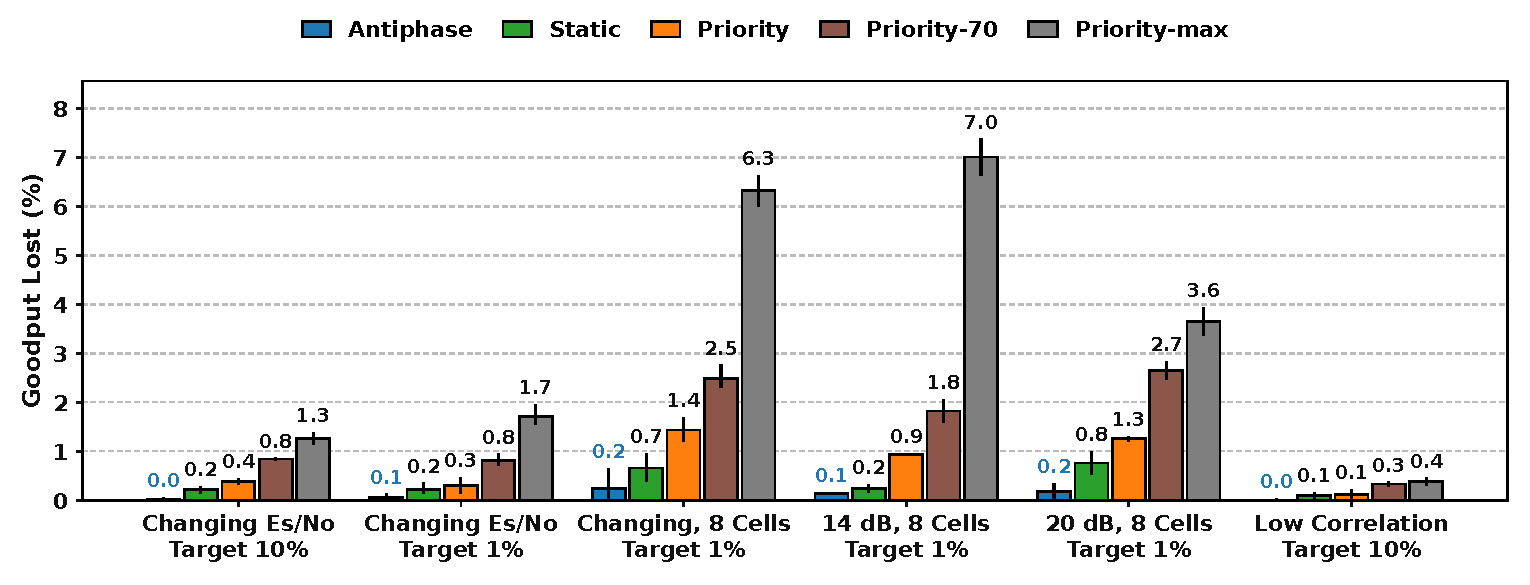
\includegraphics[width=\linewidth]{figures/eval_closed_vary.pdf}
\caption{Goodput of the two-user cells that each policy loses in other settings of the outer loop. Changing
Es/No: every two-user cell moves between 14, 16, and 20~dB and stays 2~s at a value. 8 Cells: eight two-user
cells. Low correlation: the low-correlation channel at 6~dB. Lines show the range over seeds.}
\label{fig:vary}
\end{figure}

\begin{table}[t]
\caption{Closed-loop link adaptation in twelve more settings. Cells: AI served (tokens/s) / goodput of the
two-user cells against the same server without AI. Busy: share of the time in which the neural receivers run
without AI. Rows without a cell count have four two-user cells.}
\label{tab:esno}
\footnotesize
\setlength{\tabcolsep}{2.5pt}
\begin{tabular}{@{}lrrrrrrr@{}}
\toprule
Setting, target & Gain & Busy & \sys & Fixed 10\% & 30\% share & 70\% share & No cap \\
\midrule
Changing Es/No, 10\% & $+$12.5\% & 70\% & 10.4k / 0.0\% & 4.7k / $-$0.2\% & 11.3k / $-$0.4\% & 24.6k / $-$0.8\% & 30.1k / $-$1.3\% \\
Changing Es/No, 1\% & $+$28.4\% & 35\% & 34.4k / $-$0.1\% & 5.6k / $-$0.2\% & 18.1k / $-$0.3\% & 42.9k / $-$0.8\% & 49.1k / $-$1.7\% \\
Changing Es/No, 8 cells, 1\% & $+$25.5\% & 58\% & 17.4k / $-$0.2\% & 5.1k / $-$0.7\% & 13.9k / $-$1.4\% & 33.0k / $-$2.5\% & 43.8k / $-$6.3\% \\
14~dB, 10\% & $+$13.9\% & 80\% & 6.1k / $-$0.1\% & 4.3k / $-$0.4\% & 10.0k / $-$0.7\% & 20.7k / $-$1.3\% & 25.8k / $-$2.5\% \\
14~dB, 1\% & $+$18.2\% & 39\% & 31.5k / $-$0.1\% & 5.4k / $-$0.1\% & 17.0k / $-$0.2\% & 41.2k / $-$0.6\% & 49.2k / $-$2.2\% \\
14~dB, 8 cells, 1\% & $+$15.6\% & 60\% & 15.5k / $-$0.1\% & 4.9k / $-$0.2\% & 13.3k / $-$0.9\% & 31.3k / $-$1.8\% & 45.2k / $-$7.0\% \\
20~dB, 10\% & $+$10.8\% & 55\% & 18.7k / 0.0\% & 5.0k / $-$0.1\% & 13.5k / $-$0.1\% & 31.2k / $-$0.4\% & 36.2k / $-$0.5\% \\
20~dB, 1\% & $+$40.2\% & 29\% & 38.5k / $+$0.1\% & 5.7k / $+$0.1\% & 19.3k / 0.0\% & 45.3k / $-$0.5\% & 50.5k / $-$0.6\% \\
20~dB, 8 cells, 1\% & $+$39.5\% & 58\% & 17.2k / $-$0.2\% & 5.0k / $-$0.8\% & 13.5k / $-$1.3\% & 31.9k / $-$2.7\% & 38.3k / $-$3.7\% \\
Low correlation, 10\% & $+$4.3\% & 52\% & 21.7k / 0.0\% & 5.1k / $-$0.1\% & 14.2k / $-$0.1\% & 33.3k / $-$0.3\% & 39.1k / $-$0.4\% \\
Low correlation, 1\% & $+$8.4\% & 16\% & 47.8k / 0.0\% & 6.0k / 0.0\% & 22.9k / 0.0\% & 50.4k / 0.0\% & 52.6k / 0.0\% \\
Low correlation, 8 cells, 1\% & $+$8.6\% & 33\% & 36.2k / 0.0\% & 5.5k / 0.0\% & 18.5k / 0.0\% & 43.7k / $-$0.2\% & 49.6k / $-$0.2\% \\
\bottomrule
\end{tabular}
\end{table}

\noindent\textbf{Other SNRs, Another Channel, and a Changing Channel.} The results above use one channel at
one Es/No. We generate the slots of MCS 10-16 for the high-correlation channel at 14 and 20~dB and for the
low-correlation channel at 6~dB, and we let the Es/No of a two-user cell change: a cell stays 2~s at 14, 16,
or 20~dB and then moves to another value at random, at times that differ between the cells. The outer loop
does not know the channel and follows the outcomes. Table~\ref{tab:esno} and Figure~\ref{fig:vary} show the
twelve settings. \sys loses at most 0.2\% of the goodput in all of them, also when the Es/No changes; with
the nine settings of Table~\ref{tab:closedloop} this makes 21 settings with a loss of at most 0.4\%. The
shares lose by setting: the 30\% share 0.0-1.4\%, the 70\% share 0.0-2.7\%, and low priority alone
0.0-7.0\%. The large losses are those of the high-correlation channel with eight two-user cells, at 14~dB,
at 20~dB, and with a changing Es/No. On the low-correlation channel the recovery path adds 4-9\% and a lost
recovery costs little: no share loses more than 0.4\%, and \sys serves 1.5-2.1$\times$ the AI of the 30\%
share because the neural receivers run for 16-52\% of the time. The AI that \sys serves follows the idle
time of the neural receivers in all settings: against the 30\% share it serves 0.6$\times$ at 20\% idle
time (14~dB at the 10\% target, where the share pays 0.7\% of the goodput), 0.9-1.0$\times$ at 30-32\%,
1.2-1.5$\times$ at 40-48\%, and 1.9-2.1$\times$ from 61\%. In the twelve settings the neural receiver
adds 1.45-1.62~ms to the 99.9th percentile of the layer-1 latency of the single-user cells, \sys adds
0.00-0.13~ms on top, the 30\% share 0.23-0.34~ms, and low priority alone 0.60-0.89~ms.

\begin{table}[t]
\caption{Closed-loop link adaptation in 21 further settings: an Es/No that changes in every slot, two channels
on one server, the low-correlation channel at two more Es/No values, and the urban micro channel. Cells as in
Table~\ref{tab:esno}. Rows without a cell count have four two-user cells.}
\label{tab:more}
\footnotesize
\setlength{\tabcolsep}{2.5pt}
\begin{tabular}{@{}lrrrrrr@{}}
\toprule
Setting, target & Gain & \sys & Fixed 10\% & 30\% share & 70\% share & No cap \\
\midrule
Slow change, 10\% & $+$13.1\% & 11.3k / $-$0.1\% & 4.8k / $-$0.2\% & 11.6k / $-$0.3\% & 25.7k / $-$0.9\% & 30.7k / $-$1.4\% \\
Slow change, 1\% & $+$29.0\% & 36.9k / 0.0\% & 5.7k / $-$0.1\% & 18.8k / $-$0.2\% & 44.2k / $-$0.4\% & 50.2k / $-$1.0\% \\
Slow change, 8 cells, 1\% & $+$27.7\% & 18.9k / $-$0.3\% & 5.1k / $-$0.5\% & 14.2k / $-$1.1\% & 33.8k / $-$1.9\% & 42.6k / $-$3.6\% \\
Random change, 10\% & $+$12.9\% & 10.2k / 0.0\% & 4.7k / $-$0.3\% & 11.2k / $-$0.4\% & 24.2k / $-$1.0\% & 29.4k / $-$1.6\% \\
Random change, 1\% & $+$27.9\% & 36.4k / $-$0.1\% & 5.7k / $-$0.2\% & 18.7k / $-$0.4\% & 44.3k / $-$1.0\% & 50.0k / $-$1.5\% \\
Random change, 8 cells, 1\% & $+$24.7\% & 20.3k / $-$0.2\% & 5.2k / $-$0.5\% & 14.7k / $-$1.2\% & 35.4k / $-$2.0\% & 43.7k / $-$3.7\% \\
Fast change, 10\% & $+$13.8\% & 12.0k / $-$0.1\% & 4.8k / $-$0.2\% & 11.6k / $-$0.3\% & 25.7k / $-$0.8\% & 30.3k / $-$1.2\% \\
Fast change, 1\% & $+$28.7\% & 37.1k / 0.0\% & 5.7k / $-$0.1\% & 18.8k / $-$0.2\% & 44.1k / $-$0.5\% & 50.1k / $-$1.1\% \\
Fast change, 8 cells, 1\% & $+$26.5\% & 19.3k / $-$0.1\% & 5.1k / $-$0.5\% & 14.2k / $-$0.7\% & 33.6k / $-$1.5\% & 42.3k / $-$3.3\% \\
Mixed channels, 10\% & $+$7.8\% & 15.2k / 0.0\% & 4.9k / $-$0.1\% & 12.6k / $-$0.2\% & 29.4k / $-$0.5\% & 34.5k / $-$0.5\% \\
Mixed channels, 1\% & $+$18.5\% & 41.1k / 0.0\% & 5.7k / 0.0\% & 20.1k / 0.0\% & 46.6k / $-$0.2\% & 51.5k / $-$0.3\% \\
Mixed channels, 8 cells, 1\% & $+$17.8\% & 23.3k / $-$0.2\% & 5.2k / $-$0.4\% & 15.1k / $-$0.5\% & 36.9k / $-$1.6\% & 45.2k / $-$3.1\% \\
Low correlation 4.5~dB, 10\% & $+$5.5\% & 11.0k / $-$0.2\% & 4.6k / $-$0.1\% & 11.3k / $-$0.3\% & 24.7k / $-$0.6\% & 30.3k / $-$0.9\% \\
Low correlation 4.5~dB, 1\% & $+$4.1\% & 49.5k / 0.0\% & 6.1k / 0.0\% & 24.0k / 0.0\% & 51.0k / 0.0\% & 52.8k / 0.0\% \\
Low correlation 4.5~dB, 8 cells, 1\% & $+$4.6\% & 40.6k / 0.0\% & 5.7k / 0.0\% & 20.1k / $-$0.1\% & 46.0k / $-$0.1\% & 51.0k / $-$0.2\% \\
Low correlation 7.5~dB, 10\% & $+$5.5\% & 27.3k / 0.0\% & 5.2k / 0.0\% & 15.8k / 0.0\% & 37.0k / $-$0.3\% & 43.0k / $-$0.3\% \\
Low correlation 7.5~dB, 1\% & $+$6.8\% & 48.6k / 0.0\% & 6.0k / 0.0\% & 23.4k / 0.0\% & 50.5k / 0.0\% & 52.8k / 0.0\% \\
Low correlation 7.5~dB, 8 cells, 1\% & $+$6.6\% & 38.8k / 0.0\% & 5.6k / 0.0\% & 19.6k / 0.0\% & 44.4k / $-$0.1\% & 50.2k / $-$0.1\% \\
Urban micro, 10\% & $+$5.3\% & 24.4k / 0.0\% & 5.2k / 0.0\% & 15.3k / 0.0\% & 35.7k / $-$0.1\% & 41.6k / $-$0.3\% \\
Urban micro, 3\% & $+$1.5\% & 36.9k / 0.0\% & 5.6k / 0.0\% & 18.4k / 0.0\% & 43.6k / 0.0\% & 49.4k / $-$0.3\% \\
Urban micro, 8 cells, 3\% & $+$1.4\% & 16.1k / $-$0.1\% & 4.8k / $-$0.1\% & 13.1k / $-$0.1\% & 29.4k / $-$0.3\% & 37.1k / $-$0.7\% \\
\bottomrule
\end{tabular}
\end{table}

\noindent\textbf{A Continuously Changing Channel, Mixed Channels, and a Third Channel.} We extend the settings
in three directions (Table~\ref{tab:more}). First, the Es/No of a cell changes in every slot. We add white
noise to slots generated at 20~dB: the noise variance of the generator is $1.267\cdot10^{-e/10}$ at an Es/No
of $e$~dB for every MCS and channel, and the added variance sets the Es/No of each slot. Slots made in this way
at 16 and 14~dB match generated slots within 2.9 percentage points of decoded TBs, for both receivers and at
all seven MCS levels. The Es/No moves between 14 and 20~dB with a period of 5.12~s (slow, up to 3.7~dB/s) or
1.28~s (fast, up to 14.7~dB/s), or it follows a random process with a mean of 16.5~dB, a standard deviation of
1.75~dB, and a correlation time of 1~s. \sys loses 0.0-0.3\% of the goodput in the nine settings, and the
shares lose up to 3.7\%; the order of the policies and the size of the losses are those of the fixed channel.
At the 10\% target the outer loop follows all three trajectories: its mean MCS rises by about two levels from
the lowest to the highest Es/No, and 8.7-13.3\% of the TBs need a retransmission at every Es/No. At the 1\%
target it does not follow the fast change, where its MCS moves by 0.4 levels and 2.4\% of the TBs need a
retransmission at the lowest Es/No; the comparison of the policies is the same. Second, half of the two-user
cells of a server use the high-correlation channel at 16~dB and half the low-correlation channel at 6~dB. The
loss of a share falls on the high-correlation cells: with eight two-user cells at the 1\% target, the 70\%
share loses 1.6\% on average, 3.1\% in the high-correlation cells and 0.2\% in the others, and low priority
alone loses 6.4\% and 0.2\%. \sys loses 0.4\% and 0.0\%. Thus, a cap must be chosen for the worst cell of a
server. Third, we run the low-correlation channel at 4.5 and 7.5~dB and the urban micro channel at 10~dB. The
recovery path adds 4-9\% on the low-correlation channel and 1-5\% on the urban micro channel, and a lost
recovery costs little there: the shares lose at most 0.9\% and 0.7\%, and \sys at most 0.2\% and 0.1\%. On
the urban micro channel the conventional receiver fails 1.5\% of the TBs at the lowest MCS; we use a 3\%
target, at which the outer loop stays at the lowest MCS. Across the three channels the gain of the recovery
path and the goodput that a share pays move together: 11-40\% and up to 8.2\%, 4-9\% and up to 0.9\%, and
1-5\% and up to 0.7\%. With the 21 settings above, \sys loses at most 0.4\% of the goodput in 42 settings with
one configuration; two measurements exceed 0.3\%, both with eight two-user cells (0.32\% and 0.34\%). We
measured the setting with the largest loss, eight two-user cells at the 1\% target, in four campaigns: the ten
runs give 0.28\% on average, and 0.0-0.7\% by campaign.

\begin{table}[t]
\caption{AI on a slice of the SMs of a GPU (a CUDA green context), with the outer loop (two seeds). Cells as in
Table~\ref{tab:esno}; settings by the number of two-user cells and the target. Slice $N$: \sys with the AI of a GPU on $N$ SMs while the neural receiver of that GPU
runs. Always 28: the AI runs on 28 SMs at all times. Each block is one campaign with its own run of \sys.}
\label{tab:slice}
\footnotesize
\setlength{\tabcolsep}{1.6pt}
\begin{tabular}{@{}lrrrrrrr@{}}
\toprule
\multicolumn{8}{@{}l}{\emph{Neural receivers on all 108 SMs}} \\
Setting & \sys & Slice 12 & Slice 16 & Slice 28 & Always 28 & 30\% share & 70\% share \\
\midrule
4 cells, 10\% & 11.8k / 0.0\% & 8.8k / $-$0.1\% & 11.7k / $-$0.2\% & 13.6k / $-$0.3\% & 8.8k / $-$0.2\% & 11.4k / $-$0.2\% & 25.7k / $-$0.7\% \\
4 cells, 1\% & 33.7k / $-$0.1\% & 28.5k / $-$0.1\% & 31.7k / $-$0.2\% & 33.4k / $-$0.5\% & 13.2k / $-$0.2\% & 17.7k / $-$0.3\% & 41.9k / $-$0.8\% \\
8 cells, 1\% & 16.8k / 0.0\% & 13.9k / $-$1.0\% & 16.9k / $-$0.9\% & 20.6k / $-$1.9\% & 10.2k / $-$1.2\% & 13.9k / $-$1.9\% & 34.0k / $-$3.6\% \\
\bottomrule
\end{tabular}

\vspace{4pt}
\begin{tabular}{@{}lrrrrr@{}}
\toprule
\multicolumn{6}{@{}l}{\emph{Neural receivers off the slice (on 92 or 80 SMs), or AI at normal priority}} \\
Setting & \sys & Slice 16, off & Slice 28, off & Always 28, normal & Always 28, off \\
\midrule
4 cells, 10\% & 11.6k / $+$0.1\% & 12.2k / $-$0.1\% & 18.0k / $-$0.5\% & 11.6k / $-$0.4\% & 12.8k / $-$0.5\% \\
4 cells, 1\% & 33.5k / 0.0\% & 31.7k / $-$0.4\% & 36.5k / $-$0.9\% & 15.4k / $-$0.7\% & 15.6k / $-$0.7\% \\
8 cells, 1\% & 17.2k / $-$0.7\% & 17.8k / $-$1.7\% & 25.7k / $-$3.3\% & 13.4k / $-$3.2\% & 13.6k / $-$3.3\% \\
\bottomrule
\end{tabular}
\end{table}

\noindent\textbf{An SM Slice Does Not Replace the Rule.} A GPU can also be divided in space. A CUDA green
context gives a process a set of the SMs of a GPU; Weaver~\cite{weaver} divides a GPU between LDPC decoding
and AI training in this way. We build green contexts into the AI workers and the neural receiver processes
and measure two uses (Table~\ref{tab:slice}). First, as a baseline, the AI always runs on 28 of the 108 SMs:
with low priority, with normal priority, or with the neural receivers on the other 80 SMs. In all nine cases
this loses more goodput than \sys in the same campaign, 0.2-3.3\%, and it serves 0.4-1.1$\times$ the AI,
because the AI stays on 26\% of the GPU when the neural receivers are idle. Second, as an option of \sys, the
AI of a GPU moves to a slice of 12, 16, or 28 SMs while the neural receiver of that GPU runs, and it is not
stopped. With 28 SMs the option serves 1.0-1.2$\times$ the AI of the default and loses 0.3-1.9\% of the
goodput; with the neural receivers on the other 80 SMs it serves 1.1-1.6$\times$ and loses 0.5-3.3\%. Slices
of 12 and 16 SMs serve no more AI than the default. The loss follows the run time of the neural receiver,
whatever divides the GPU. The policies with a median run of 6.4-6.6~ms (\sys) lose 0.0-0.7\%, those with
6.8-7.2~ms lose 0.1-1.9\%, and those with 7.4-7.9~ms lose 0.4-3.6\%, shares and slices alike. This is the
path of the model (Section~\ref{sec:model}): a run has 1.2~ms of slack, and the neural receiver alone takes
0.84~ms longer on 80 SMs than on 108. A slice isolates the AI, and the neural receiver needs the SMs. The AI
gains little on a slice next to a running neural receiver: a piece takes 7.1$\times$ its bound on the whole
GPU on 28 shared SMs and 4.0$\times$ on 28 SMs of its own. In runs of 100~s, the option with 28 SMs adds
0.23~ms to the 99.9th percentile of the layer-1 latency, and the default adds 0.06~ms. The fixed split with
the neural receivers on 80 SMs lowers this percentile to 0.25~ms below the server without AI, because the
conventional receivers no longer share 28 SMs with the neural receiver, and it loses 8.3\% of the recoveries.
The default of \sys has no slice.

\subsection{Protection and latency}
\label{sec:protect}

\noindent\textbf{Takeaway.} In steady state \sys adds 0.04-0.06~ms to the 99.9th-percentile L1 latency and
0.07-0.09~ms to the run of the neural receiver, 2.8-21$\times$ and 5.2-19$\times$ less than the baselines.
After the start of a run, 3 of 3.2 million TBs pass the layer-1 deadline with \sys, and its AI requests
finish within their limit at the 99th percentile.

\begin{figure}[t]
\centering
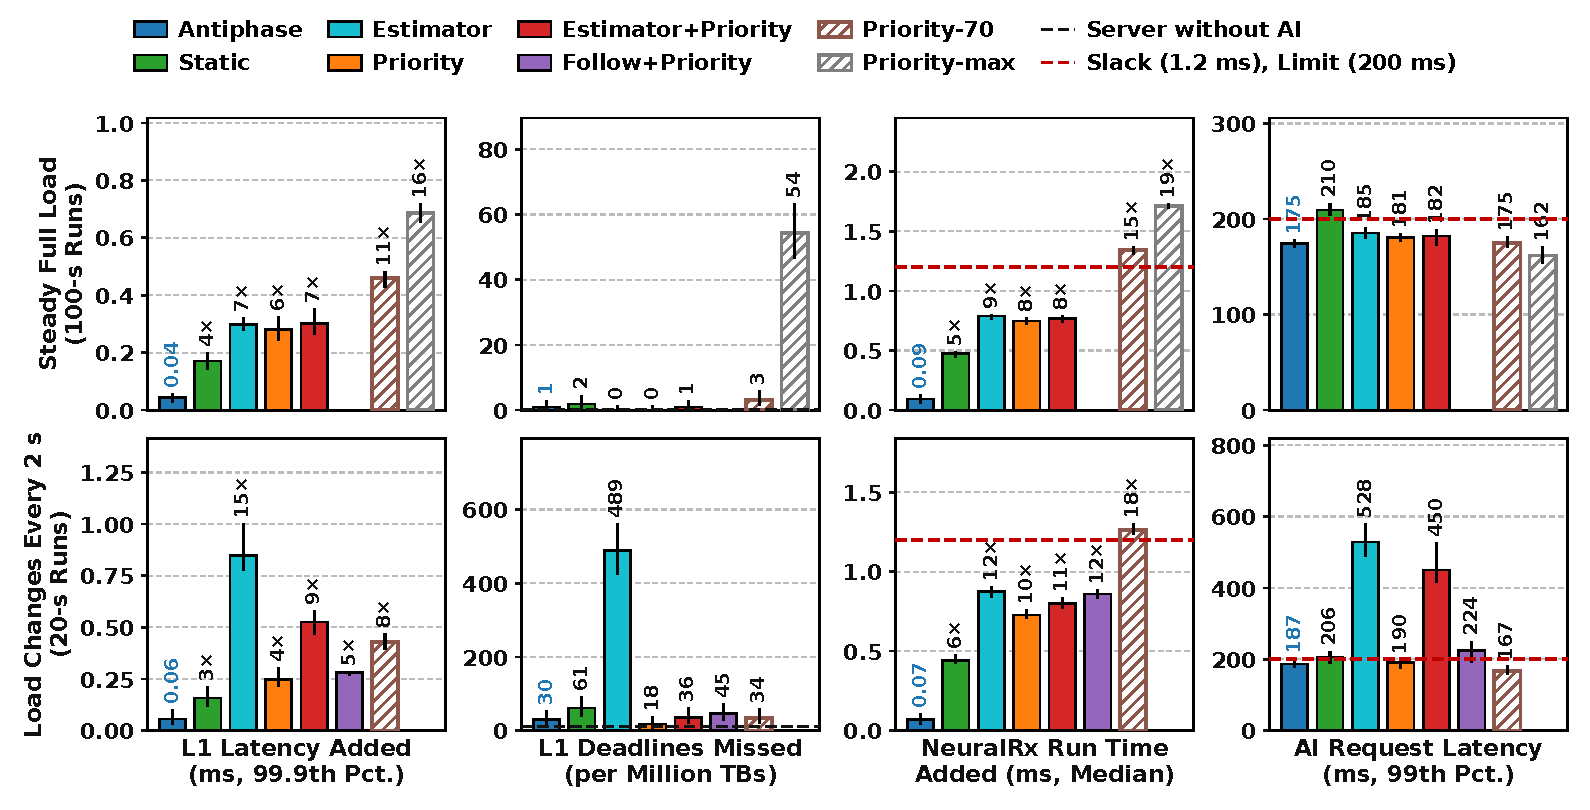
\includegraphics[width=\linewidth]{figures/eval_protect.pdf}
\caption{What AI adds to the latency of the radio work, and the latency of the AI requests (16 cells, four
GPUs, five seeds; lines: range over seeds, for the misses the 95\% interval). Top: runs of 100~s without
their first 20~s. Bottom: runs of 20~s without their first 5~s. L1 latency: samples arrive until the
conventional result. The number on a baseline is how many times more it adds than \sys.}
\label{fig:protect}
\end{figure}

\begin{table}[t]
\caption{Scheduling metrics at a steady full load (16 cells, four GPUs; five runs of 100~s per policy without
their first 20~s, 3.2 million TBs per policy). L1 latency and neural receiver run time are in ms; AI latency
is from the arrival of a request to the end of its prefill, in ms. cuPHY alone: a server without the neural
receiver and without AI.}
\label{tab:sched}
\footnotesize
\setlength{\tabcolsep}{3.2pt}
\begin{tabular}{@{}lrrrrrrrr@{}}
\toprule
Policy & AI served & Recoveries & L1 latency & TBs past & NeuralRx run & AI latency & Requests & GPU \\
 & (k tokens/s) & kept (\%) & p50 / p99.9 & L1 deadline & p50 / p99 & p50 / p99 & rejected (\%) & idle (\%) \\
\midrule
cuPHY alone & -- & -- & 1.38 / 1.49 & 0 & -- & -- & -- & -- \\
No AI & 0.0 & 100.0 & 1.39 / 3.01 & 0 & 6.28 / 6.57 & -- & -- & 26.4 \\
\sys & 34.1 & 99.9 & 1.81 / 3.06 & 3 & 6.38 / 6.82 & 77 / 175 & 16.4 & 1.0 \\
\textit{Static} & 5.6 & 99.3 & 1.47 / 3.18 & 6 & 6.76 / 7.05 & 120 / 210 & 64.9 & 2.1 \\
\textit{Estimator} & 11.0 & 98.7 & 1.54 / 3.31 & 0 & 7.07 / 7.36 & 84 / 185 & 46.8 & 1.4 \\
\textit{Priority} & 17.6 & 98.8 & 1.61 / 3.29 & 0 & 7.03 / 7.29 & 79 / 181 & 33.9 & 1.5 \\
\textit{Estimator+Priority} & 17.6 & 98.7 & 1.62 / 3.31 & 3 & 7.05 / 7.31 & 77 / 182 & 33.8 & 1.4 \\
\textit{Priority-70} & 42.6 & 94.3 & 1.80 / 3.47 & 10 & 7.63 / 7.98 & 73 / 175 & 9.2 & 1.1 \\
\textit{Priority-max} & 48.9 & 93.7 & 1.90 / 3.70 & 174 & 8.00 / 8.53 & 61 / 162 & 4.0 & 1.7 \\
\bottomrule
\end{tabular}
\end{table}

\begin{table}[t]
\caption{TBs past the layer-1 deadline by the time since the start of a run (runs of 100~s; five per policy
with 16 cells and with one GPU, three with 20 and 48 cells).}
\label{tab:when}
\footnotesize
\begin{tabular}{@{}lrrrr@{}}
\toprule
Policy & First 5~s & 5-10~s & 10-20~s & After 20~s \\
\midrule
\multicolumn{5}{@{}l}{\emph{16 cells, four GPUs (3.2 million TBs after 20~s)}} \\
No AI & 125 & 14 & 0 & 0 \\
\sys & 113 & 7 & 8 & 3 \\
\textit{Static} & 74 & 11 & 2 & 6 \\
\textit{Estimator} & 40 & 19 & 7 & 0 \\
\textit{Priority} & 101 & 11 & 0 & 0 \\
\textit{Estimator+Priority} & 74 & 8 & 0 & 3 \\
\textit{Priority-70} & 185 & 13 & 13 & 10 \\
\textit{Priority-max} & 167 & 41 & 19 & 174 \\
\multicolumn{5}{@{}l}{\emph{4 cells, one GPU (0.8 million TBs after 20~s)}} \\
No AI & 23 & 0 & 0 & 0 \\
\sys & 64 & 2 & 1 & 0 \\
\textit{Static} & 48 & 2 & 0 & 46 \\
\textit{Priority} & 41 & 0 & 0 & 21 \\
\multicolumn{5}{@{}l}{\emph{20 cells, four GPUs (three runs, 2.3 million TBs after 20~s)}} \\
No AI & 88 & 0 & 0 & 2 \\
\sys & 99 & 0 & 2 & 3 \\
\textit{Static} & 54 & 4 & 0 & 0 \\
\textit{Priority} & 70 & 5 & 0 & 1 \\
\multicolumn{5}{@{}l}{\emph{48 cells at one third load, four GPUs (three runs, 1.9 million TBs after 20~s)}} \\
No AI & 30 & 0 & 0 & 17 \\
\sys & 70 & 0 & 0 & 17 \\
\textit{Static} & 42 & 10 & 3 & 26 \\
\textit{Priority} & 64 & 11 & 3 & 14 \\
\bottomrule
\end{tabular}
\end{table}

Figure~\ref{fig:protect} and Table~\ref{tab:sched} give the metrics of a scheduler: what AI adds to the
latency of the radio work, the deadlines missed, the latency of the AI requests, and the use of the GPU time.
The values at full load are from runs of 100~s (40,000 uplink slots per cell), measured in one job with the
policies in turn.

\begin{table}[t]
\caption{Layer-1 latency of the single-user cells, whose workload is the same at every level (runs with the
outer loop of Section~\ref{sec:worth}; 20~s per run without the first 5~s; range over four settings). Room:
time left to the 4.0~ms deadline at the 99.9th percentile.}
\label{tab:levels}
\footnotesize
\begin{tabular}{@{}lrrr@{}}
\toprule
Server & Median (ms) & 99.9th percentile (ms) & Room (ms) \\
\midrule
Conventional receiver alone & 1.39-1.41 & 1.50-1.52 & 2.48-2.50 \\
+ neural receiver, no AI & 1.40-2.09 & 3.05-3.10 & 0.90-0.95 \\
+ AI, \sys & 1.88-2.07 & 3.12-3.14 & 0.86-0.88 \\
+ AI, \textit{Static} & 1.50-2.17 & 3.22-3.31 & 0.69-0.78 \\
+ AI, \textit{Priority} & 1.70-2.31 & 3.37-3.41 & 0.59-0.63 \\
+ AI, \textit{Priority-70} & 1.85-2.41 & 3.48-3.56 & 0.44-0.52 \\
+ AI, \textit{Priority-max} & 1.95-2.54 & 3.73-4.00 & 0.00-0.27 \\
\bottomrule
\end{tabular}
\end{table}

\noindent\textbf{Three Levels.} The latency of the radio work on an AI-RAN server is not zero at any level,
and we separate what the neural receiver adds from what AI adds. Table~\ref{tab:levels} compares the
single-user cells, whose workload does not change, on a server with the conventional receiver alone, with the
neural receiver, and with AI. The neural receiver adds 1.53-1.59~ms to the 99.9th percentile of the layer-1
latency, because the conventional receiver of a GPU slows while the neural receiver of that GPU runs. This
takes 62-64\% of the room to the deadline and leaves 0.90-0.95~ms. It is the price of the recovery path,
which raises the goodput by 11-31\% (Section~\ref{sec:worth}). AI must fit into the room that is left. \sys
adds 0.03-0.07~ms. \textit{Static} adds 0.17-0.21~ms, \textit{Priority} adds 0.30-0.36~ms, and
\textit{Priority-max} adds 0.68-0.90~ms, which leaves 0.00-0.27~ms. We repeated the 10\% target, where the
neural receivers run for 68\% of the time, in runs of 100~s (three seeds, 1.15 million TBs of single-user
cells per level after the first 20~s). No TB passes the layer-1 deadline with the conventional receiver alone
or with the neural receiver, and 3 do with \sys. \textit{Priority} serves the same AI as \sys in this
setting (11.5k tokens/s); it adds 0.29~ms to the 99.9th percentile against 0.03~ms, loses 4.2\% of the
recoveries against 0.9\%, and 11 TBs pass the deadline. With \textit{Priority-max} the 99.99th percentile is
4.20~ms and 470 TBs pass the deadline. On the low-correlation channel at 6~dB the levels are the same (three
runs of 100~s): 1.49~ms with the conventional receiver alone, 3.13~ms with the neural receiver, and 3.13~ms
with \sys, which serves 21.1k tokens/s with 4 late TBs of 1.15 million. \textit{Priority} serves 14.3k and
leaves 0.61~ms of room against 0.87~ms, and \textit{Priority-max} has 505 late TBs and a 99.99th percentile of
4.21~ms. At a steady full load with a fixed MCS (first rows of
Table~\ref{tab:sched}), the conventional receiver alone has 1.49~ms at the 99.9th percentile and the neural
receiver raises it to 3.01~ms. In the rest of this section, the server without AI is the second level: it
runs the neural receiver.

\noindent\textbf{Start of a Run.} The processes of a run start cold, and its first seconds are not the steady
state. Table~\ref{tab:when} counts the TBs past the layer-1 deadline by the time since the start. Without
AI, 139 TBs are late in five runs, and all of them are in the first 10~s. With \sys, 128 of 131 are in the
first 20~s. The runs of 10-40~s in the rest of this section include this start: their layer-1 misses of
0.02-0.04\% occur with and without AI, and they compare the policies at an equal run length, not in steady
state.

\noindent\textbf{L1 Latency.} In steady state a TB is decoded in 3.01~ms at the 99.9th percentile without AI,
0.99~ms before the layer-1 deadline. \sys adds 0.04~ms. \textit{Static} adds 0.17~ms, \textit{Priority} and
the two estimator policies 0.28-0.30~ms, \textit{Priority-70} 0.46~ms, and \textit{Priority-max} 0.69~ms. At
the 99.99th percentile \sys equals the server without AI (3.18~ms), and the baselines are at 3.34-3.94~ms.
After the first 20~s, no TB of 3.2 million is late without AI, three are late with \sys, at most ten with the
baselines that cap the share, and 174 with \textit{Priority-max}. With one GPU, no TB of 0.8 million is late
after the first 20~s without AI or with \sys, and \textit{Static} and \textit{Priority} miss the deadline for
46 and 21 TBs. With 20 cells, \sys has 3 late TBs of 2.3 million against 2 without AI, and with 48 cells 17 of
1.9 million against 17. In all four settings the late TBs of \sys after the start are those of the server
without AI. When the load changes, the two estimator policies add 0.53-0.87~ms, because their share is one
second behind the load, and \textit{Estimator} misses the deadline for 0.05\% of the TBs; \sys adds
0.04-0.06~ms. \sys raises the
median L1 latency from 1.39 to 1.81~ms, as much as \textit{Priority-70}, because the two smaller unit classes
run next to the conventional receivers; with only the smallest class next to them the median rises by
0.20~ms (Section~\ref{sec:rules}). The tail does not move.

\noindent\textbf{Neural Receiver.} A run of the neural receiver takes 6.28~ms at the median without AI
and 6.38~ms with \sys. The baselines add 0.44-1.71~ms. \textit{Priority-70} and \textit{Priority-max}
are beyond the slack of 1.2~ms (Equation~\ref{eq:slack}), which is where they lose recoveries.

\noindent\textbf{AI Latency.} The AI requests have a limit of 200~ms. With \sys the 99th percentile of the
request latency is 175-187~ms, and 99.0-99.8\% of the placed requests finish within the limit. At a steady
full load the baselines are at 162-210~ms: \textit{Request Dispatcher} places a request only if a GPU can
finish it in time, and a policy with less GPU time rejects more requests, 16\% with \sys, 34\% with
\textit{Priority}, and 65\% with \textit{Static}. When the load changes, the two estimator policies take
388-528~ms. The rejections follow the offered load: at 27k tokens/s offered, \sys rejects 0.6\% of the
requests and has a 99th-percentile latency of 115~ms (Section~\ref{sec:cells}).

\noindent\textbf{GPU Time.} Without AI, the GPUs have no work on them for 26.4\% of the time at full load
and for 37-43\% under the two changing loads. With \sys they have no work for 1.0-4.0\%. Every policy
with AI keeps the GPUs busy for 89-99\% of the time; the policies differ in what the busy time does to the
radio work. An AI piece is on a GPU next to a running neural receiver for 1.4-2.4\% of the time with \sys,
the unit that finishes after a stop, and for 19-38\% with the baselines.

\subsection{What each rule adds}

\noindent\textbf{Takeaway.} Stoppable AI pieces and no AI next to a running neural receiver raise the
recoveries kept from 97.8\% to 100.0\%. Keeping the largest AI units away from the conventional receivers
lowers the layer-1 misses from 0.061\% to 0.036\%.
\label{sec:rules}

\begin{table}[t]
\caption{Rules changed one at a time (16 cells at full load, 53k tokens/s offered; five seeds, rows marked
$^{*}$ two). Without AI: layer-1 misses 0.032\%, lost candidates 1.6\%, three-slot runs 10\%.}
\label{tab:rules}
\footnotesize
\begin{tabularx}{\linewidth}{@{}>{\raggedright\arraybackslash}Xrrrrr@{}}
\toprule
Configuration & AI & Recoveries & Layer-1 & Lost & Three-slot \\
 & tokens/s & kept & misses & candidates & runs \\
\midrule
Low-priority AI, no grants & 49.0k & 93.7\% & 0.044\% & 6.4\% & 88\% \\
Grants without stops, AI next to a neural receiver while three are free$^{*}$ & 39.5k & 97.8\% & 0.025\% & 3.2\% & 52\% \\
Stops, AI next to a neural receiver while one is free$^{*}$ & 44.0k & 95.1\% & 0.066\% & 5.2\% & 81\% \\
Stops, while two are free$^{*}$ & 42.2k & 96.6\% & 0.051\% & 4.1\% & 64\% \\
Stops, while three are free & 39.8k & 99.3\% & 0.038\% & 2.4\% & 35\% \\
Stops, no AI next to a neural receiver & 37.6k & 100.0\% & 0.061\% & 1.8\% & 14\% \\
+ largest units not next to the conventional receivers (\sys) & 34.1k & 99.9\% & 0.036\% & 1.7\% & 11\% \\
\bottomrule
\end{tabularx}
\end{table}

Table~\ref{tab:rules} changes the rules one at a time.

\noindent\textbf{Stops.} Without stops, AI is still running for 43\% of the neural receiver time during
which the rule wants it off, the neural receiver takes 7.04~ms at the median, and 52\% of the runs take three
slots. With stops the figure is 6-7\%, the time until the group on the GPU ends, and the neural receiver
takes 6.38~ms against 6.28~ms alone.

\noindent\textbf{AI Next to a Neural Receiver.} Allowing AI next to a running neural receiver while $R$
neural receivers of the server are free trades recoveries for AI. From no AI next to a neural receiver to
$R = 3$, 2, and 1, the three-slot runs grow from 14\% to 35\%, 64\%, and 81\%, the lost candidates from 1.8\%
to 2.4\%, 4.1\%, and 5.2\%, and the AI served from 37.6k to 44.0k tokens/s. \sys uses no AI next to a neural
receiver: it keeps the recoveries of the run without AI and has no value to set for the number of GPUs. The
event simulation gives a difference of 0.1 points between this rule and $R = 3$ and the measurement gives
0.6, a difference inside the model error.

\noindent\textbf{Unit Sizes Next to the Conventional Receivers.} With every size class allowed next to the
conventional receivers, the layer-1 misses rise to 0.061\%: next to 1,024-token units the conventional
receivers of four cells finish in 4.05~ms at the 99.9th percentile. Keeping the largest class away from
them returns the misses to 0.036\% and costs 9\% of the AI served. Two variants that choose the classes by
the number of active cells of the GPU did not help. Allowing only the smallest class when five cells are
active and none above, as a calibration with five cells per GPU suggests, cut the AI served by 28-51\% with
20, 32, and 48 cells and left the layer-1 misses unchanged: the calibration runs the neural receiver and AI
next to the conventional receivers at once, which \sys never does. Allowing the largest class while at most
two or three cells are active served 0-19\% less AI under a changing load, because a request that has
picked large chunks waits when more cells become active. The size classes next to the conventional receivers
also set the median L1 latency: it is 1.40~ms without AI, 1.60~ms with only the smallest class next to them
(24.2k tokens/s served), 1.82~ms with the two smaller classes (33.9k), and 1.83~ms with every class (37.3k).
The 99.9th percentile is the same without AI and with one or two classes (3.07-3.12~ms) and 3.51~ms with
every class. \sys allows two classes because the layer-1 decode has a deadline; a deployment that needs a
lower median changes this parameter and no rule.

\subsection{Distance to a clairvoyant schedule}
\label{sec:clairvoyant}

\noindent\textbf{Takeaway.} \sys turns 70\% of the GPU time that is safe for AI into served tokens, which
is 1.9-6.4$\times$ the existing mechanisms that keep the recoveries.

\begin{figure}[t]
\centering
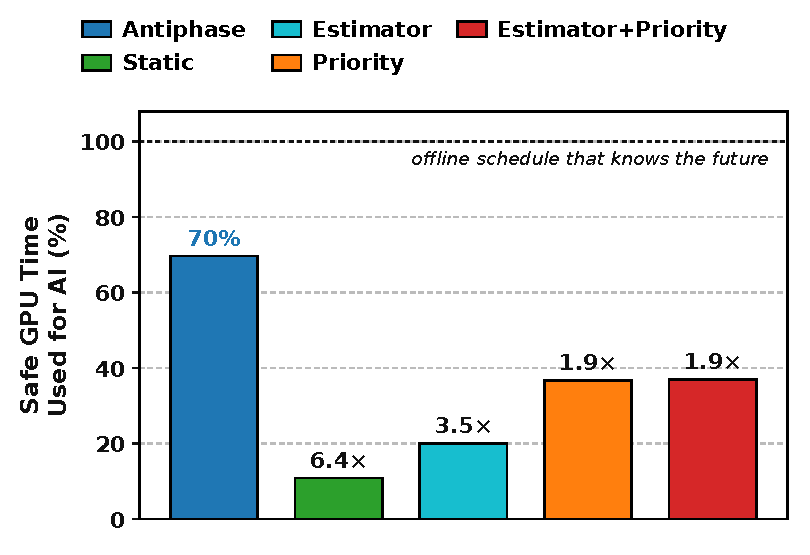
\includegraphics[width=0.6\linewidth]{figures/eval_gpu_use.pdf}
\caption{Share of the GPU time that is safe for AI that each policy turns into served tokens at a steady
full load (16 cells, four GPUs). 100\% is an offline schedule that knows every later failure and loses no
recovery. The number on a baseline is the factor of \sys over it.}
\label{fig:use}
\end{figure}

\begin{table}[t]
\caption{Share of the GPU time in which AI may run with no recovery lost, computed on the runs without AI,
and AI served. The clairvoyant AI served scales the measured AI served of \sys by the AI time and is at most
what \textit{Priority-max} serves (full load) or the offered load.}
\label{tab:clairvoyant}
\footnotesize
\setlength{\tabcolsep}{3.5pt}
\begin{tabular}{@{}lrrrrrrr@{}}
\toprule
 & Neural & \multicolumn{3}{c}{AI time} & \multicolumn{2}{c}{AI served (tokens/s)} & \sys\ / \\
Setting & receiver busy & rule, ideal & \sys & clairvoyant & \sys & clairvoyant & clairvoyant \\
\midrule
16 cells, full load & 36\% & 64\% & 62\% & 96.5\% & 34.1k & 49.0k & 70\% \\
16 cells, load alternates & 27\% & 73\% & 69\% & 98.1\% & 41.4k & 53.0k & 78\% \\
16 cells, random steps & 22\% & 78\% & 72\% & 98.9\% & 44.7k & 53.0k & 84\% \\
Two two-user cells & 18\% & 82\% & 77\% & 99.6\% & 46.6k & 53.0k & 88\% \\
Eight two-user cells & 67\% & 33\% & 33\% & 76.1\% & 11.8k & 27.3k & 43\% \\
Two GPUs, 8 cells & 34\% & 66\% & 61\% & 93.8\% & 16.6k & 25.6k & 65\% \\
One GPU, 4 cells & 30\% & 70\% & 59\% & 94.6\% & 8.5k & 13.2k & 64\% \\
32 cells, half load & 37\% & 63\% & 62\% & 97.5\% & 33.4k & 52.6k & 63\% \\
\bottomrule
\end{tabular}
\end{table}

The comparisons above are with other online policies. Table~\ref{tab:clairvoyant} compares \sys with an
offline schedule that knows every later candidate. We compute it on the runs without AI. The schedule keeps
the start time of every neural receiver run and loses no candidate. It runs AI next to a neural
receiver for as long as the run still ends before the next run on that receiver starts; a run next to AI
advances at 0.786 of its speed alone. For fixed start times this schedule is optimal: assigning each run to
the receiver whose stretched run ends first minimizes the time that AI must be off.

\noindent\textbf{The Rule Is Implemented Tightly.} At full load the neural receivers run for 36\% of the GPU
time. The rule of \sys allows AI for the other 64\%, and AI is on the GPU for 62\%: stops and grants cost
two points.

\noindent\textbf{What Knowledge of the Future Is Worth.} The clairvoyant schedule turns AI off for 3.5\% of
the time: only 13\% of the runs must be cut for a later candidate. \sys serves 70\% of the clairvoyant AI
at full load, 78-88\% at lower loads, and 43\% with eight two-user cells. The existing mechanisms that keep
at least 98.8\% of the recoveries serve 11-37\% at full load, and allowing AI next to a neural receiver
while three are free serves 81\% and loses 0.7\% of the recoveries. The gap is one of information. Which
neural receiver is needed two slots later is known only when that slot is decoded, 5.0~ms into the run; AI
next to the run until then has delayed it by 1.07~ms of the 1.2~ms slack, less than the stop latency and the
spread of the run length leave. A rule that spends the slack lost 4.0\% of the recoveries in our runs.
Closing the gap needs a prediction of the failures two slots ahead; the correlation between the failures of
consecutive slots (0.19-0.26 against a mean of 0.145) is too weak for it.

\subsection{Neural receiver demand and server size}

\noindent\textbf{Takeaway.} From one to four GPUs, \sys serves 6.4-7.8$\times$ the AI of \textit{Static} and
1.9-2.2$\times$ that of \textit{Priority} (Figure~\ref{fig:sizes}a). With more two-user cells, the neural
receivers run for more of the time and the factor falls: from 8.2$\times$ to 2.7$\times$ over
\textit{Static} and from 2.1$\times$ to 1.0$\times$ over \textit{Priority}, which loses 4.0\% of the
recoveries with eight two-user cells where \sys loses 0.4\% (Figure~\ref{fig:sizes}c).

\begin{figure}[t]
\centering
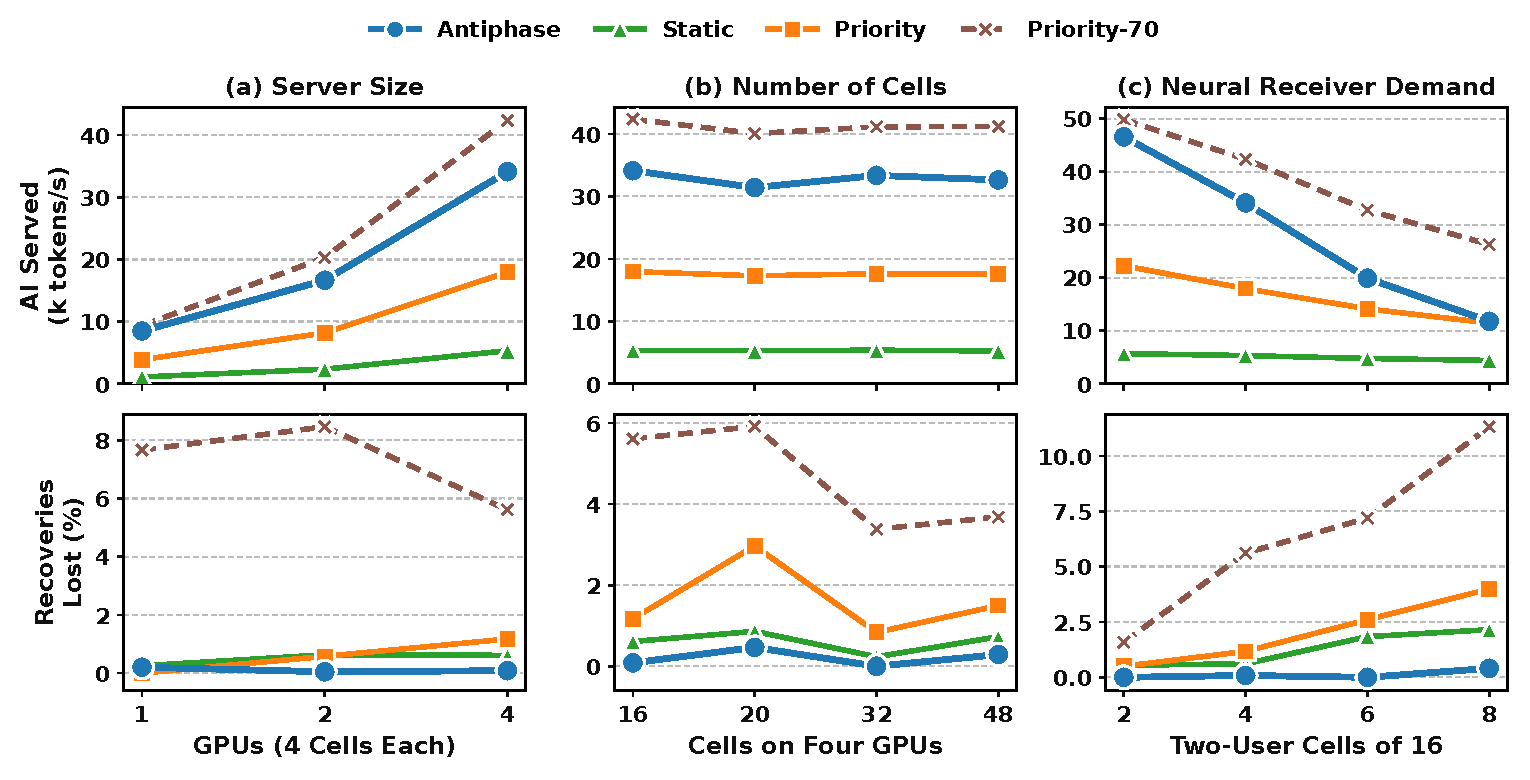
\includegraphics[width=\linewidth]{figures/eval_scale.pdf}
\caption{AI served (top) and recoveries lost (bottom) at full load for (a) one, two, and four GPUs with one
two-user cell per GPU, (b) 16-48 cells on four GPUs, and (c) two to eight two-user cells of sixteen.
\textit{Priority-70} (dashed) serves more AI and loses 1.6-11.3\% of the recoveries.}
\label{fig:sizes}
\end{figure}

\begin{table}[t]
\caption{Neural receiver demand and server size at full load, 32 requests/s offered per GPU (two seeds;
16 cells with four two-user cells and the two settings with one GPU: five). Each cell shows AI tokens/s and
recoveries kept.}
\label{tab:scale}
\footnotesize
\setlength{\tabcolsep}{4.5pt}
\begin{tabular}{@{}lrllll@{}}
\toprule
GPUs, cells, two-user cells & Recovered TBs/s, no AI & \sys & Fixed 10\% & 30\%, low priority & 70\%, low priority \\
\midrule
4, 16, 2 & 101 & 46.6k, 100.0\% & 5.7k, 99.5\% & 22.3k, 99.5\% & 49.8k, 98.4\% \\
4, 16, 4 & 187 & 34.1k, 99.9\% & 5.3k, 99.4\% & 18.0k, 98.8\% & 42.4k, 94.4\% \\
4, 16, 6 & 283 & 19.9k, 100.0\% & 4.8k, 98.2\% & 14.1k, 97.4\% & 32.8k, 92.8\% \\
4, 16, 8 & 359 & 11.8k, 99.6\% & 4.4k, 97.8\% & 11.5k, 96.0\% & 26.3k, 88.7\% \\
2, 8, 2 & 95 & 16.6k, 100.0\% & 2.4k, 99.4\% & 8.2k, 99.4\% & 20.3k, 91.5\% \\
2, 8, 4 & 154 & 6.9k, 99.9\% & 2.0k, 99.2\% & 5.8k, 96.6\% & 14.2k, 88.3\% \\
1, 4, 1 & 39 & 8.5k, 99.8\% & 1.1k, 99.7\% & 3.9k, 100.0\% & 9.3k, 92.3\% \\
1, 4, 2 & 64 & 4.5k, 97.7\% & 1.0k, 97.5\% & 2.9k, 96.8\% & 8.1k, 84.1\% \\
\bottomrule
\end{tabular}
\end{table}

\noindent\textbf{Demand.} Table~\ref{tab:scale} raises the neural receiver demand by making more cells
two-user cells. With two and four GPUs, \sys keeps at least 99.6\% of the recoveries in all six settings
and serves 2.7-8.2$\times$ the AI of \textit{Static} and 1.0-2.1$\times$ that of the 30\% share with
low-priority AI. \sys gives GPU time back as the demand grows: the neural receivers run for a larger part
of the time, and the AI served falls from 46.6k tokens/s with two two-user cells to 11.8k with eight. The
70\% share with low-priority AI serves 1.1-2.2$\times$ the AI of \sys and loses 1.6-11.7\% of the recoveries.

\noindent\textbf{GPUs.} The rule of \sys has no value that depends on the number of neural receivers
(Figure~\ref{fig:sizes}). With one GPU and one two-user cell, \sys serves 8.5k tokens/s at 99.8\%, and the
70\% share with low-priority AI serves 9.3k at 92.3\%. With one GPU and two two-user cells, one neural
receiver cannot serve the demand: 31\% of the candidates are lost without AI. \sys then keeps 97.7\% of the
recoveries, the level of \textit{Static} and of \textit{Priority}, and serves
1.6-4.5$\times$ their AI. With one GPU, \sys misses the layer-1 deadline for 0.04-0.06\% of the TBs against
0.02-0.04\% without AI in these runs of 10~s. The difference comes from the start of the runs: in runs of
100~s no TB is late after the first 20~s with \sys or without AI, and \textit{Static} and \textit{Priority}
miss the deadline for 46 and 21 of 0.8 million TBs (Table~\ref{tab:when}).

\subsection{More cells and other loads}

\noindent\textbf{Takeaway.} With 20, 32, and 48 cells on four GPUs, \sys serves 5.9-6.2$\times$ the AI of
\textit{Static} and 1.8-1.9$\times$ that of \textit{Priority}, and it loses at most 0.5\% of the
recoveries (Figure~\ref{fig:sizes}b).
\label{sec:cells}

\begin{table}[t]
\caption{More cells on four GPUs, 53k tokens/s offered (four seeds). Each cell shows AI tokens/s, recoveries
kept, and layer-1 misses.}
\label{tab:cells}
\footnotesize
\begin{tabular}{@{}llll@{}}
\toprule
Policy & 20 cells, full load & 32 cells, half load & 48 cells, one third load \\
\midrule
\sys & 31.4k, 99.5\%, 0.044\% & 33.4k, 100.0\%, 0.041\% & 32.6k, 99.7\%, 0.130\% \\
Fixed 10\% & 5.3k, 99.1\%, 0.037\% & 5.4k, 99.8\%, 0.038\% & 5.3k, 99.3\%, 0.125\% \\
Fixed 30\%, low-priority AI & 17.3k, 97.0\%, 0.035\% & 17.6k, 99.2\%, 0.048\% & 17.6k, 98.5\%, 0.112\% \\
Fixed 70\%, low-priority AI & 40.1k, 94.1\%, 0.054\% & 41.1k, 96.6\%, 0.051\% & 41.2k, 96.3\%, 0.117\% \\
No AI & 0, 100\%, 0.032\% & 0, 100\%, 0.037\% & 0, 100\%, 0.090\% \\
\bottomrule
\end{tabular}
\end{table}

\noindent\textbf{Cells.} Table~\ref{tab:cells} keeps four GPUs and adds cells: 20 cells at full load, five
per GPU, and 32 and 48 cells where each cell carries a TB in a slot with probability 0.5 and 0.33. \sys
serves 31.4k-33.4k tokens/s and keeps 99.5-100.0\% of the recoveries, 5.9-6.2$\times$ the AI of the fixed
10\% share and 1.8-1.9$\times$ that of \textit{Priority}. The 70\% share with low-priority
AI serves 23-28\% more and loses 3.4-5.9\% of the recoveries. In these runs of 10~s, \sys misses the
layer-1 deadline for 0.044\% and 0.041\% of the TBs with 20 and 32 cells against 0.032\% and 0.037\% without
AI, and with 48 cells every policy with AI misses it more often than the run without AI (0.11-0.13\% against
0.09\%). These misses come from the start of the runs. In runs of 100~s without their first 20~s, \sys
has 3 late TBs of 2.3 million with 20 cells and 17 of 1.9 million with 48 cells, against 2 and 17 without AI
(Table~\ref{tab:when}), and it adds 0.03~ms to the 99.9th-percentile L1 latency where \textit{Static} and
\textit{Priority} add 0.16-0.25~ms. With 48 cells, up to 12 cells of a GPU are active in one slot, and
nine TBs per million are late with and without AI.

\begin{table}[t]
\caption{Lost candidates with 20 cells for two time bounds of the neural receiver (two seeds). The
prediction is the closed form with the arrivals and run lengths measured at 8.6~ms, computed before the
runs at 7.6~ms. \sys here allows only the smallest unit class next to five active cells.}
\label{tab:bound}
\footnotesize
\begin{tabular}{@{}lrrrrr@{}}
\toprule
Policy & Measured, & Predicted, & Measured, & Three-slot runs, & Three-slot runs, \\
 & 8.6~ms & 7.6~ms & 7.6~ms & predicted & measured \\
\midrule
No AI & 3.6\% & 1.6\% & 1.6\% & 11\% & 17\% \\
\sys & 6.4\% & 1.8\% & 1.8\% & 15\% & 18\% \\
30\%, low-priority AI & 6.8\% & 3.1\% & 3.8\% & 43\% & 47\% \\
70\%, low-priority AI & 7.0\% & 5.7\% & 6.2\% & 92\% & 92\% \\
\bottomrule
\end{tabular}
\end{table}

\noindent\textbf{Choosing the Time Bound with the Model.} With 20 cells, a time bound of 8.6~ms for the
neural receiver gives a latest start time of 2.9~ms and a slack of 0.05~ms in Equation~\ref{eq:slack}.
Without AI, 47\% of the runs take three slots, and every policy loses 3-5\% of the recoveries. Before we
ran a bound of 7.6~ms, we computed its loss with the closed form from the arrivals and run lengths measured
at 8.6~ms. Table~\ref{tab:bound} compares the prediction with the runs: it is within 0.7 points for all four
policies. With the bound of 7.6~ms, the run without AI recovers 190 TBs per second against 185, and at most
0.2\% of the neural receiver runs end after the recovery deadline.

\noindent\textbf{AI Load.} With 13k and 27k tokens/s offered at a full radio load of 16 cells, \sys serves
every request and keeps 99.4-99.8\% of the recoveries: it rejects 0.0\% and 0.6\% of the requests, and the
99th percentile of the request latency is 77 and 115~ms. At 27k offered, \textit{Priority} serves 18.9k and
rejects 13.2\%. The 16\% of requests that \sys rejects at 53k offered are the load above its capacity. At 106k tokens/s offered, every policy serves less
than at 53k: the admission accepts shorter requests, which take more GPU time per token. \sys serves 24.3k
tokens/s at 100.0\%, and \textit{Priority-70} serves 27.9k at 93.6\%. When AI requests arrive
in bursts (inter-arrival times with a coefficient of variation of 4), \sys serves 23.3k tokens/s at 99.5\%,
\textit{Static} 3.6k at 99.0\%, and \textit{Priority-70} 27.4k at 95.9\%.

\subsection{Several kinds of AI work}
\label{sec:kinds}

\noindent\textbf{Takeaway.} With four models and five kinds of AI work on every GPU, the same rule keeps
99.7\% of the recoveries. \sys serves 1.5$\times$ the chat tokens and 3.1$\times$ the larger-LLM tokens of
\textit{Priority}.

\begin{table}[t]
\caption{Five kinds of AI work on every GPU (16 cells at full load, three seeds, every policy in one job).
Chat: output tokens/s on time, and in parentheses the responses with every token on time and the rejected
requests. Larger LLM: prompt tokens/s within the limit and rejected requests.}
\label{tab:kinds}
\footnotesize
\begin{tabular}{@{}lrlllll@{}}
\toprule
Policy & Recoveries & Chat & Larger LLM & Embedding & Image & Filler \\
 & kept & & & items/s & items/s & tokens/s \\
\midrule
\sys & 99.7\% & 119 (92\%, 10\%) & 3.7k (11\%) & 593 & 237 & 5.4k \\
Fixed 10\% & 99.3\% & 6 (0\%, 64\%) & 0.0k (67\%) & 117 & 36 & 3.0k \\
Fixed 30\%, low-priority AI & 98.5\% & 81 (31\%, 29\%) & 1.2k (28\%) & 542 & 210 & 3.9k \\
Fixed 30\% & 97.3\% & 95 (55\%, 25\%) & 2.2k (24\%) & 572 & 224 & 4.6k \\
Fixed 70\%, low-priority AI & 96.5\% & 141 (100\%, 2\%) & 4.5k (2\%) & 593 & 237 & 12.8k \\
Low-priority AI, no cap & 94.0\% & 154 (100\%, 0\%) & 4.6k (0\%) & 594 & 238 & 18.6k \\
\bottomrule
\end{tabular}
\end{table}

Every GPU runs five kinds of AI work with four models: chat with Qwen2.5-1.5B (prefill, then up to 64 output
tokens; first token within 200~ms, every later token within 50~ms; 0.8 requests/s), prefill with
Qwen2.5-3B (400~ms; 2 requests/s), text embedding (50~ms; 150 items/s), image classification (50~ms; 60
items/s), and a filler of 1,024-token prefill without a limit. The work with a limit needs 65\% of the GPU
time. Table~\ref{tab:kinds} shows the result.

\sys keeps 99.7\% of the recoveries with the rule unchanged. It serves every embedding and image item, 80\%
of the larger-LLM prompt tokens and 77\% of the chat output tokens that \textit{Priority-max} serves, and 92\%
of its chat responses have every token on time. Against the mechanisms that keep at least 98.5\% of the
recoveries, \sys serves 1.5$\times$ the chat output tokens of \textit{Priority}, with
92\% against 31\% of the responses fully on time, and 3.1$\times$ the larger-LLM tokens. \sys serves less of
the work without a limit: \textit{Priority-70} and \textit{Priority-max} serve 2.4-3.4$\times$
the filler tokens, at 3.2-5.7 points fewer recoveries. \sys rejects 10\% of the chat requests and 11\% of the
larger-LLM requests, because the AI of a GPU stops for 6.4~ms while its neural receiver runs. With chat
alone (1.5 requests/s per GPU, two seeds), \sys serves 258 output tokens/s with every response on time and
keeps 99.7\%, and \textit{Priority-max} serves 300 and keeps 97.2\%.

\subsection{Choosing the TBs to recover}

On the urban micro channel, sending every failed TB to the neural receiver takes 4,891-4,926 runs and
recovers 663-757 TBs without AI. Sending only the TBs of slots with at most nine failed code blocks takes
651-777 runs and recovers 589-746 TBs: 85\% fewer runs for 5\% fewer recoveries. On the low-correlation
channel with eight two-user cells, the neural receivers cannot take every failed TB. Sending only slots
with at most three failed code blocks removes 40\% of the runs and 22\% of the recoveries and raises the
recoveries per run from 0.77 to 0.99.

\section{Related Work}

\noindent\textbf{GPU sharing in vRAN and AI-RAN.} YinYangRAN~\cite{yinyangran} multiplexes LDPC decoding
with other workloads by MPS shares that a learned reliability estimator changes at intervals of at least
one second. CloudRIC~\cite{cloudric} pools accelerators for LDPC decoding, and
Concordia~\cite{concordia} reserves capacity for vRAN tasks. Weaver~\cite{weaver} shares the GPU of a RAN
server between LDPC decoding and the training of foundation models with CUDA green contexts, which give each
side a set of streaming multiprocessors (SMs), and it sets the SMs of the radio per slot from the MCS and the
PRBs. Its radio work is LDPC decoding without a neural receiver. We build the same means into our code: a
neural receiver that gives up 26\% of the SMs runs 15\% longer, which is 70\% of its slack, and AI that
stays on a slice of the SMs loses more goodput than \sys (Section~\ref{sec:worth}). AI-RAN
studies~\cite{interplay,caora,haf,distributedairan} place AI and RAN workloads across servers. Their radio
work has one deadline and no second receiver. \sys adds a recovery path with its own deadline, and our
evaluation includes a share chosen by an estimator and a share that follows the load as baselines.

\noindent\textbf{GPU scheduling.} DARIS, REEF, XSched, and nvtaskset~\cite{daris,reef,xsched,nvtaskset}
schedule GPU stages, kernels, or contexts by priority, and Orion~\cite{orion} runs best-effort GPU work when
it does not interfere with a high-priority job. SMEC~\cite{smec} sets MPS priorities on an edge server that
is separate from the RAN server. These systems protect the latency of the running high-priority job. Our
model shows that this is not the quantity that decides the recoveries: a neural receiver that meets its
deadline still costs recoveries when it holds its GPU for one more slot. \sys decides from the state of
every neural receiver, and our evaluation includes low priority as a baseline.

\noindent\textbf{Neural receivers.} DeepRx~\cite{deeprx} and the NVlabs receivers~\cite{nrx5g,nrxrt} design
and train neural receivers, ARCHES~\cite{arches} switches between an AI channel estimator and a conventional
one, and OCUDU~\cite{ocudu} exposes timing classes in the distributed unit. These works report receiver
gains against their own baselines. We compare at equal LDPC effort with a production receiver and study the
neural receiver as a workload that shares the GPU with AI.

\noindent\textbf{Loss models.} Loss systems describe servers without a waiting room~\cite{harcholbalter}.
Our model is a loss system in which the service time counts in uplink slots, the arrivals of consecutive
slots are dependent, and the policy enters through the distribution of the run length.

\section{Limitations}

The channels are the synthetic channels of the public NVlabs configuration, and every cell replays 512
slots. \sys serves 43-88\% of the AI of a clairvoyant schedule; it does not predict which neural receiver
will be needed. The larger model allows four to five cells per GPU at full load; 32 and 48 cells run when half or
two thirds of the cells are idle, and with 48 cells nine TBs per million miss the layer-1 deadline in steady
state with and without AI. The recovery deadline follows from the TDD pattern and the PUSCH preparation time~\cite{ts38214} and
is not validated with a layer-2 stack; the goodput results apply a retransmission
schedule to measured TB records and do not run HARQ. The outer loop runs on three channels at seven Es/No values,
with an Es/No that changes in steps and continuously, and with two channels on one server; the continuous
change adds noise to generated slots, and the channel itself is replayed. On the urban micro channel the outer
loop stays at the lowest MCS at the 3\% target. The goodput that the shares with more AI give up is
0.3-0.6 percentage points at a fixed MCS and at most 2.5\% with the outer loop at a 10\% target; it reaches
8.2\% at a 1\% target, and it is at most 0.9\% on the low-correlation channel and 0.7\% on the urban micro channel. The closed form takes the run lengths of the neural receiver from
runs of the policy; it does not predict them from the policy. The baselines are the mechanisms of prior
systems on our code: the estimator follows the published design, with our reliability definition and
without the look-ahead of the full system. \sys raises the median L1 latency by 0.4~ms. \sys serves less
AI without a time limit than \textit{Priority-max}. The layer-1 misses of 0.02-0.13\% in the runs of 10-40~s
come from the cold start of the prototype, with and without AI. The steady-state counts are from 0.8-3.2
million TBs per setting and do not establish a reliability beyond 99.999\%; the changing loads and 32 cells
are not measured in runs of 100~s. The SM slices have a fixed size, two seeds, and one AI model, and we
build them with the driver API because the MPS of this server cannot divide the SMs; we do not run Weaver.
All runs use one GPU model.

\section{Conclusion}

A neural receiver that decodes more TBs than a production receiver at equal LDPC effort takes twice the
uplink period. Running it as a recovery path next to AI inference loses recoveries by a path that deadline
checks miss: a failed TB cannot wait, and a neural receiver that AI slows by more than the slack of 1.2~ms
holds its GPU for one more uplink slot. A loss model of this path agrees with 672 runs within 0.82
percentage points on average. \sys stops the low-priority AI of a GPU when its neural receiver starts and
keeps the largest AI units away from the conventional receivers. Under three load patterns with mixed
channels, \sys serves 6.4-7.5$\times$ the AI of a fixed 10\% GPU share and 1.2-1.9$\times$ that of a share
chosen by a load estimator with low-priority AI, and it keeps 99.9\% of the recoveries. In steady state it
adds 0.04-0.06~ms to the 99.9th-percentile latency of the layer-1 decode, and after the start of a run its
TBs pass the layer-1 deadline as rarely as those of the server without AI. It turns 70\% of
the GPU time that is safe for AI into served tokens, 1.9-6.4$\times$ the existing mechanisms that keep the
recoveries. With an outer-loop
rate controller, lost recoveries lower the MCS: the cost in goodput reaches 2.5\% at a 10\% retransmission
target and 8\% at a 1\% target with a neural receiver demand near the capacity. \sys loses at most 0.4\% of
the goodput in 42 settings with one configuration, which include three channels and a continuously changing
SNR, and no fixed or low-priority GPU share does.

\bibliographystyle{ACM-Reference-Format}
\bibliography{references}

\end{document}
